\documentclass[12pt,a4paper]{report}

% Packages
\usepackage{settings}


\addbibresource{references.bib} %Import the bibliography file

% Page setup
\geometry{a4paper, margin=1in}
\setstretch{1.5} % Line spacing

%%%%%%%%%%%%%%%%%%

% Title page information
\title{\textbf{LLM-Use in Academic Writing -- An Estimation}}
\author{Lena Holzwarth\\MSc Kognitionswissenschaft}
\date{Month Year}

%%%%%%%%%%%%%%%%%%
\begin{document}
%%%%%%%%%%%%%%%%%%

\selectlanguage{english} 

%%%%%%%%%%%%%%%%%%

\begin{titlepage}
 \begin{center}
  {\LARGE University of T\"ubingen}\\
  {\large Faculty of Science \\
    Wilhelm Schickard Institute for Computer Science\\[4cm]}
  {\huge Master Thesis Cognitive Science\\[2cm]}
  {\Large\textbf{LLM-Use in Academic Writing -- An Estimation}\\[1.5cm]}
  {\large Lena Holzwarth\\MSc Kognitionswissenschaft}\\[0.5cm]
  May 2026\\[3cm]
  {\small\bf Reviewers}\\[0.5cm]
  \parbox{7cm}{\begin{center}{\large Prof. Dr. Dmitry Kobak}\\
  {\footnotesize Department of
Mathematics, \\Computer Science, and Statistics\\
	Ghent University}\end{center}}\hfill\parbox{7cm}{\begin{center}
  {\large Prof. Dr. Michael Franke}\\
  General Linguistics \& Pragmatics\\
  {\footnotesize Department of Linguistics\\
	University of T\"ubingen}\end{center}
 }
  \end{center}
\end{titlepage}


% Title page

\thispagestyle{empty}
\vspace*{\fill}
\begin{minipage}{11.2cm}
\textbf{Holzwarth, Lena:}\\
\emph{LLM-Use in Academic Writing -- An Estimation}\\ Master Thesis Cognitive Science\\
University of T\"ubingen\\
Thesis period: 09.01.2026 -- 08.07.2026
\end{minipage}
\newpage



%%%%%%%%%%%%%%%%%%
\chapter*{Abstract}
In the past years, LLM-powered Chatbots have grown from relative obscurity to wide-spread usage. Their ability to generate high-quality text makes them a valuable tool for researchers. The use of LLMs to write or edit papers has been argued to remove language barriers for non-natively English speaking (NNES) scholars but also inspires concerns about misuse and fraud.  Because of this, attempts have been made at estimating the prevalence of LLM-altered text in scientific publications. Kobak et al. (2025) use word frequencies to track LLM-use in biomedical abstracts, showing that certain style words occurred at much higher rates after the release of ChatGPT. By calculating the difference between the observed and counter-factual frequency based on predictions from pre-2023, they obtain a lower bound for LLM-use. This thesis expands on their work by introducing a stronger lower bound, yielding estimates of up to 89\% of papers in Pubmed Central (PMC) being written with the help of LLMs. In tests on simulated data, the metric was found to accurately retrieve the underlying fraction of LLM-use. LLMs were more likely to be used in the body of a paper than in the abstract, but different sections within the body showed few differences in usage, except for the discussion, which yielded the highest estimates among the different sections. LLM-use was found to be relatively uniform in the introduction and discussion sections, and more clustered in the methods. In accordance with prior research, papers from NNES were more likely to have been processed with LLMs. Our estimation method yielded higher usage rates than most of the previous literature, although many surveys among scientists report LLM-use close to our estimates. 



%%%%%%%%%%%%%%%%%%
\selectlanguage{ngerman} 
\chapter*{Zusammenfassung}

In den letzten Jahren haben sich LLM-gestützte Chatbots von relativer Unbekanntheit zu einer weit verbreiteten Nutzung entwickelt. Ihre Fähigkeit, qualitativ hochwertigen Text zu generieren, macht sie zu einem wertvollen Werkzeug, u. A. für Forschende. Der Einsatz von LLMs zum Verfassen oder Bearbeiten wissenschaftlicher Arbeiten kann Sprachbarrieren für nicht-englischsprachige Wissenschaftler (NNES) beseitigen, weckt jedoch auch Bedenken hinsichtlich Missbrauch und Betrug.  Deshalb wurden Versuche unternommen, das Ausmaß durch LLMs veränderter wissenschaftlicher Publikationen abzuschätzen. Kobak et al.(2025) nutzen Wortfrequenzen, um die LLM-Nutzung in biomedizinischen Abstracts nachzuverfolgen, und zeigen, dass bestimmte Stilwörter nach der Veröffentlichung von ChatGPT deutlich häufiger vorkommen. Durch die Berechnung der Differenz der beobachteten und der kontrafaktischen Häufigkeit auf der Grundlage von Vorhersagen aus der Zeit vor 2023 erhalten sie eine Untergrenze der LLM-Nutzung. Diese Arbeit baut auf ihren Ergebnissen auf, indem sie eine strengere Untergrenze einführt, die zu Schätzungen führt, wonach bis zu 89\% der Artikel in Pubmed Central (PMC) mithilfe von LLMs verfasst wurden. In Tests mit simulierten Daten zeigt sich, dass die Metrik den zugrunde liegenden Anteil der LLM-Nutzung genau schätzt. LLMs wurden eher im Hauptteil einer Arbeit als im Abstract verwendet, doch zeigten die verschiedenen Abschnitte innerhalb des Hauptteils kaum Unterschiede in der Nutzung, mit Ausnahme der Diskussion, die unter den verschiedenen Abschnitten die höchsten Schätzwerte ergab. Die LLM-Nutzung erwies sich in den Abschnitten ``Einleitung'' und ``Diskussion'' als relativ gleichmäßig und war im Abschnitt ``Methoden'' stärker konzentriert. In Übereinstimmung mit früheren Untersuchungen wurden Artikel von NNES mit höherer Wahrscheinlichkeit mit LLMs bearbeitet. Unsere Schätzmethode ergab höhere Nutzungsraten als die meisten vorherigen Veröffentlichungen, obwohl viele Umfragen unter Wissenschaftler*Innen eine LLM-Nutzung melden, die nahe an unseren Schätzungen liegt. 


\selectlanguage{english} 
\newpage


%%%%%%%%%%%%%%%%%%
\tableofcontents
\newpage



%%%%%%%%%%%%%%%%%%
\section{Introduction}\label{sec:intro}

Since the release of OpenAI's ChatGPT\footnote{https://chatgpt.com/} in November 2022, chatbots based on Large language models (LLMs) have become ubiquitous in the public consciousness.
Due to their continued improvement, going from simple chat interfaces to fully integrated agentic systems like Anthropic's Claude Code\footnote{https://claude.com/product/claude-code}, they are increasingly helpful in any workplace dealing with writing, programming, or project planning.
One such workplace is academia, and it is not surprising that researchers across disciplines have begun to adopt LLMs for editing or writing papers, peer reviews, or grant applications \cite{Kwon2025}.
Proponents of the technology praise it as a tool for accessibility and inclusivity \cite{Bao2025_linguistic, Berdejo-Espinola2023, Prakash2025}, arguing that it enables non-native English speakers (NNES) to overcome language barriers by translating or performing grammar checks \cite{Kousha2025}.
However, the surge of ChatGPT's popularity is accompanied by concerns of misuse \cite{Liebrenz2023, Zheng2023}.
LLMs are prone to hallucination, so if their output is not thoroughly checked before using it in a paper, false or misleading statements might be published, especially if the review is also delegated to an LLM \cite{Alansari2026, Lindsay2023, Walters2023, Xu2025}.
Chatbots also make scientific fraud much easier, with the possibility of fabricating entire papers at the cost of a single prompt \cite{Kendall2024}.  
Reviewers relying on LLMs are vulnerable to hidden prompts in the paper's text, telling the LLM to give a positive review \cite{Lin2025_hidden_prompts}.
In light of these concerns, many journals have issued guidelines about the disclosure of LLM-use \cite{Brainard2023}. 
However, the perception of LLM-use leading to inaccuracies in the text, together with journals restricting or explicitly banning certain use-cases may incentivize academics against disclosing \cite{Thorp2023}.
Consequently, when trying to investigate the prevalence of LLM-use in academia, and especially in the paper-writing process, relying on self-disclosure statements will lead to underestimation \cite{Kousha2024, Kwon2025}.
\\
Regardless of the ethical concerns about using LLMs as paper-writing assistants, their prolonged use in academic text production will have an impact on academic writing as a whole.
LLMs have a distinct writing style.
Sentences generated by them have been shown to be less diverse in length \cite{Desaire2023}, but to have higher lexical diversity and positive sentiment \cite{Mak2025}.
Famously, they also show a preference for certain words, an observation which has lead to much ridicule around the most popular example ``to delve'' \cite{MacClure2024}.
The reason for this behavior is not entirely clear.
Juzek and Ward \cite{Juzek2025} replicated the training process of chatbots and tried to artificially create word preferences in the model.
They found no evidence to suggest that the training data, model architecture, or training algorithm have an influence in forming these idiosyncratic word choices.
However, the authors were able to induce an LLM with preferred words during reinforcement learning with human feedback (RLHF), the continued training scheme behind the success of modern Chatbots \cite{Bai2022}.
During RLHF, humans provide learning goals by rating the interaction with the model.
For commercial Chatbots, this work is often performed by precariously employed workers in the global south, for example in Nigeria, where ``delve'' is used much more frequently than in other English-speaking countries \cite{Perrigo2023, Hern2024}.
\\
These selective word preferences can be leveraged to estimate the proportion of LLM-processed text in a corpus.
Kobak et al. \cite{Kobak2025} track changes in word frequencies in biomedical abstracts from the PubMed database.
They compare a word's observed frequency in a given year with a projection based on its frequencies two and three years back.
The metric obtained by subtracting the predicted from the observed frequency is called excess frequency: A change in frequency that diverges from previous trends.
They identify many words that appear with excess frequency in abstracts from 2024.
This is notable, because for previous years, the observed frequency gaps are much smaller.
Because of that, a threshold can be applied to excess frequency, such that most words from pre-2024 don't exceed it, but many from 2024 do.
In addition, the majority of pre-2024 excess words are clearly related to a specific research topic, such as ``ebola'' in 2015, ``convolutional'' in 2017, or ``coronavirus'' in 2020.
In contrast, many excess words in 2024 are content-independent style words -- ``underscore'', ``potential'', ``significant'' or ``pivotal'', to name just a few.
The qualitative and quantitative differences between excess words from before and after 2024 point to a drastic shift in writing patterns that can only be explained by the adoption of LLMs into the writing process.
The identified excess style words for 2024 can therefore be interpreted as marker words for LLM-use.
It's important to note that the marker words should be applied to analyses on the corpus level and not to individual documents -- one ``delve'' does not an LLM-generated text make. 
While these words appear more frequently in LLM outputs, some of them still have very low frequency in both human and machine text.
There are texts by human authors that include them, and LLM-generated texts that don't.
\\
Using the combined excess frequencies of a selection of excess style words, Kobak et al. derive a lower bound for LLM-use estimates.
Their reasoning is quite intuitive: all instances of using one of the relevant words that go beyond the predicted frequency must have been caused by LLM-use.
Excess frequency as a metric has the advantage of not needing to distinguish between using an LLM write a whole paragraph, or suggesting changes on previously written text.
Both use-cases will lead to some LLM-suggested words being present in the final product.
\\
Here, we expand on their work on excess word frequency as a lower bound estimate of LLM-use in biomedical abstracts by making the following contributions:
\begin{itemize}
    \item \textbf{Widening the focus} from an analyzing only the abstract to the entire paper. By using the open-access PubMed Central (PMC \cite{pmc}) dataset  instead of PubMed, the proportion of LLM-assisted text in the main text of the paper can be compared with usage in the abstract, and different sections within the body can be compared against each other. 
    \item Deriving a \textbf{stronger lower bound} metric going beyond excess frequency. We show that while excess frequency is an intuitive estimate for LLM-use, it severely underestimates the true proportion of LLM-assisted text. 
    \item Computing \textbf{uncertainty measures} and performing tests on \textbf{simulated data} to increase confidence in the estimates. A disadvantage of the previous approach is the lack of a ground-truth set to test performance with. By simulating the data generation process in a Binomial model of word occurrence, we can evaluate our metric for several ground-truth levels of LLM-use.
    \item \textbf{Comparing} the LLM-use estimates with those of other estimation approaches, as well as survey data asking researchers about their LLM-use. Unlike previous studies, we find that LLM-like language has almost completely permeated academic writing.
\end{itemize}

This thesis is structured in the following way: In Section \ref{sec:related}, other approaches to estimate LLM-use in academia are discussed, such as comparable word frequency measures, word distribution modeling and LLM-detectors.
Section \ref{sec:methods} gives an overview of the data processing pipeline, the metrics used to estimate LLM-use, as well as the validation procedure employed to increase confidence in the estimates attained.
This is followed by Section \ref{sec:results}, where our estimates are reported and compared to results from other work.
Finally, the results, along with their impact and limitations are discussed in Section \ref{sec:discussion}.
\\
All code is available on GitHub\footnote{https://github.com/LenaHolzwarth/llms\_in\_academia}.
%The PMC dataset can be downloaded here\footnote{https://ftp.ncbi.nlm.nih.gov/pub/pmc/deprecated/oa\_bulk/}.
\chapter{Related Work}\label{sec:related}

Since the wide-spread proliferation of LLMs, many techniques to identify traces of LLM-use have been suggested.
As this work is focused on LLM-use specifically in academic writing, the approaches detailed here have been selected accordingly with no claim of exhaustiveness.

\section{Word frequency measures}
Most closely related to our method, word frequency measures make use of the distinct word choices separating LLM and human text production.
While not immediately visible in individual samples, these patterns emerge when looking at word distributions on the corpus level.
Reports of certain words appearing with disproportionate frequency after the introduction of ChatGPT in November 2022 have been made for publications from a wide array of scientific disciplines, ranging from linguistics \cite{Botes2025} or astronomy \cite{Astarita2024}, to medicine \cite{Matsui2024} or dentistry \cite{Uribe2024}.
\\
These observations of increased word frequency can be used to derive estimates for the prevalence of LLM-use in a given corpus, using the words with the most pronounced frequency changes as markers.
For example, Gray \cite{Gray2025} computes the relative yearly change of word frequency in papers from the Dimensions database, both for single words and word groups of up to twelve terms.
The terms are selected from a list of LLM marker words identified by Liang et al. \cite{Liang2024_review}.
Their LLM-use estimate is based on the frequency change of these excess words or word groups.
The word frequencies of 2022 are multiplied with the highest frequency increase between two consecutive pre-ChatGPT years to obtain a conservatively estimated counterfactual baseline of human word frequency. 
The number of papers with at least one of the marker words in 2023 exceeding the amount explained for by the baseline divided by the total number of papers serves as their LLM estimate.
A later study from the same author repeats the same procedure with an updated word list \cite{Gray2025}, following reports that some marker words showed decreased usage in 2024, making them less useful as LLM-use markers \cite{Geng2025}.
\\
Kousha and Thelwall \cite{Kousha2025} employ a similar approach of monitoring frequency changes of marker words in abstracts from Scopus, Web of Science and PubMed, as well as full papers from PMC, Dimensions and OpenAlex.
They select some of the marker words reported in previous research, followed by collecting additional marker words by searching for words with high co-occurrence with the pre-selected list.
While they observe strong increases in marker word frequency between the years 2022 and 2024, they don't use this to estimate the prevalence of LLM-use in their data.
However, based on their results, Gray \cite{Gray2025} derives an estimate by comparing the frequency of the word "underscore" in observed 2022 directly to its frequency in 2024 (not taking into account that human usage of the word is also subject to yearly changes).

\section{Word distribution modeling}\label{subsec:freq_model}
Similarly to the approaches detailed in the previous section, word distribution modeling makes use of distinctive word frequency patterns in LLM-generated text.
However, instead of relying only on observed frequencies in the target corpus, they model word frequencies in scientific writing as a mixture distribution of human-written and LLM-assisted text.
\\
Using a technique they call ``distributional GPT quantification'', Liang et al. \cite{Liang2024_review} analyze peer reviews of AI conference papers.
Their work is based on the observation that the fraction of LLM text in the sample can be estimated via maximum likelihood estimation (MLE) on the corpus, if the probability distributions for human and LLM-generated text are known. 
The probability distribution for human text can be estimated by counting word occurrence in texts from pre-LLM years.
To obtain the probability distribution of words in LLM-generated text, the authors prompt ChatGPT to generate alternative reviews of the conference papers from before 2023.
The authors model the distribution of all adjectives instead of relying only on marker words associated with LLM-use.
As a validation of their method, a corpus with a known fraction of LLM-generated text was constructed by sampling from the original and generated reviews. 
By computing the MLE for this corpus, the researchers are able to retrieve the correct proportion.
\\
The authors apply the same method to abstracts and introductions of scientific papers sourced from arXiv, bioRxiv and Nature portfolio journals \cite{Liang2024_paper, Liang2025}. 
LLM text is sampled by tasking ChatGPT to create a summarization outline of a paragraph from an existing, pre-ChatGPT paper, which is then given to the LLM with a prompt to generate a full paragraph based on this outline.
\\
A slightly different method is introduced by Geng and Trotta \cite{Geng2024}, who investigate LLM-use in arXiv abstracts.
Like the previous approach, they base the human word frequency baseline on pre-2023 papers and LLM frequency baseline on outputs from ChatGPT asked to polish or re-write pre-2023 abstracts.
Then, they compute a word's frequency change rate by comparing its frequencies in the original and rewritten abstracts.
The authors argue that estimates derived from a word list are more robust than those derived from single words, and further claim that the choice of the word list yielding the most accurate estimate depends on the (unknown) underlying value of LLM-use.
To find the optimal word list for each of a set of ground-truth LLM-use values to validate their procedure, they create test data with a fixed proportion of original and LLM-edited abstracts.
For each ground-truth LLM-use value, a word list is created by optimizing thresholds on word frequency and frequency change rate.
Combining the observed frequency with the simulated frequency change rate, they can derive different estimates for LLM-use in the real data using all word lists.
The mean of the estimates is taken as the preliminary result.
The estimates are then repeated with the three word lists optimized for the LLM-use proportions closest to the preliminary result.
\\
The validation procedure with ground-truth LLM-generated text is a marked advantage of these studies, compared to the frequency-based estimates, where no validation set with known distribution is available. 
However, this validation is strongly dependent upon the exact model and prompt that were used to create the LLM corpus.
The estimated distribution based on this corpus might differ drastically from the true LLM distribution, which is likely to have been created from a multitude of prompts and models.
To illustrate this point, Geng and Trotta perform validations on papers edited with a minimally different prompt than the one used to derive the frequency change rate, which leads to a systematic overestimation of true LLM-use.
While the true value is still within the error bounds, stronger alterations to the prompt or the use of a different model are likely to have a stronger impact on the estimates.

\section{LLM-detectors}
A more fine-grained approach to observing or modeling word distributions across entire corpora is to train classifiers on identifying LLM-use in individual texts. 
\\
\textbf{Zero-shot LLM detection} or model self detection uses properties of the model's idiosyncratic text generation process to determine how likely it is for a text sample to have been generated by the LLM.
An early example of this approach is \textbf{GLTR} \cite{Gehrmann2019}, which determines for every word in the text which ranking it has among the LLM's suggestions given its position in the text.
The lower the average ranking of the selected words, the more likely it is for the text to have been written by a human author.
\textbf{Detect-GPT} \cite{Mitchell2023} uses a separate LLM to generate perturbed versions of the sample and computes the log-likelihood of the original and perturbed versions under the target model. The log-likelihood of a text sample generated by the target LLM will be higher than that of the perturbed variants, while the same is not true for human-written text.
\textbf{Binoculars} \cite{Hans2024} uses a similar approach by normalizing the perplexity of a sample text under one model by the cross-perplexity of the re-generation of the sample text by a different model.
The perplexity is the negative log-likelihood of a text and can be thought of as the model's surprise, i.e. how far the text diverges from something the model would have produced. 
Binoculars has been used to check papers from the preprint platforms arXiv, bioRxiv and medRxiv \cite{Cheng2024}.
The disadvantage of these approaches is two-fold: First, in order to classify a piece of text, one needs to know with which LLM it was potentially generated, and second, one needs access to the scoring function of the LLM. 
While this is possible for some GPT variants, the scores of the most widely used model, ChatGPT, are not open to the public \cite{Mitchell2023}.
Also, these methods assume the whole text to be LLM generated, which would impede their accuracy on samples that were only partially edited with LLMs.
\\
\textbf{Trained LLM detectors} rely on a training corpus of ground-truth LLM and human text.
As an alternative to zero-shot detection, they circumvent the need for access to model parameters and can, in theory, work model-agnostically, if the training set is constructed with samples from different models.
Their performance is, however, critically dependent on the prompts and models used to generate the training corpus \cite{Liu2024_profiles}.
A common approach is to fine-tune a pretrained language model to distinguish between LLM-generated and human-written text.
Another possibility is to train conventional classifiers such as XGBoost or support vector machines on embedded representations of training text \cite{Bao2025_classifier}.
\textbf{Feature-based detectors} use linguistic features, such as the variation in sentence length, as indicators of LLM-use \cite{Desaire2023}. 
The classifier is then trained not on the texts themselves but on the features extracted from them.

There is also a plethora of proprietary LLM detectors on the market (some of which are free-to-use).
Most of them don't disclose their model architecture or training procedure.
Because of their relative convenience, many researchers investigating LLM-use in academia opt for these models to generate estimates \cite{Akram2024, Liu2024_profiles, Picazo-Sanchez2024}.
Among the models used are originality AI\footnote{https://originality.ai/}, GPTzero\footnote{https://gptzero.me/}, zeroGPT\footnote{https://www.zerogpt.com/}, GPTKit\footnote{https://gptkit.ai/}, Smodin\footnote{https://smodin.io/}, Sapling\footnote{https://sapling.ai/ai-content-detector}, Content at scale AI detector\footnote{Renamed to brandwell: https://brandwell.ai/ai-content-detector/} and Writer AI content detector\footnote{This seems to have been discontinued, the link given by the paper using it redirects to a sales pitch for the company's AI agent}.

Many concerns have been raised about current LLM-detectors' lack of accuracy \cite{Doughman2025, Lazebnik2024, Weber-Wulff2023}, going so far as to dispute even the possibility of reliable LLM-detectors \cite{Sadasivan2025}.
Early methods have been found to discriminate against non-native English speakers, disproportionately flagging their work as AI-generated, and to be unable to adjust to slight prompt changes \cite{Liang2023}.

\section{Surveying scientists}
Perhaps the most straightforward approach to evaluating the prevalence of LLM-use in academia is to ask the researchers themselves. 
Several surveys on scientists' use of AI have been conducted by publishing houses \cite{Elsevier2024, Kwon2025, Nordling2023, VanNoorden2023, Wiley2025} and independent researchers \cite{Eppler2024, Liao2024, Mishra2024, Mohammadi2026}.
These studies can be hard to compare because of different sampling pools and phrasing of questions.
An overview of questions asked in each of the surveys can be found in the Appendix \ref{ap:surveys}.
While some researchers also acknowledge the use of LLMs in their papers, the number of published papers crediting ChatGPT or similar models is much smaller than even conservative estimates of actual LLM-use \cite{Kousha2024}, emphasizing the need for anonymous surveys to produce a more accurate picture of researchers' attitudes towards the technology.
For example, in a survey done by Nature, 28\% of respondents reported to have used LLMs to edit their papers, but only 10\% disclosed their AI use \cite{Kwon2025}.

\section{Methods}\label{sec:methods}
\subsection{Dataset and Preprocessing}
\begin{figure}[htbp]
    %comment: this should be a different color than frequency
    \centering
    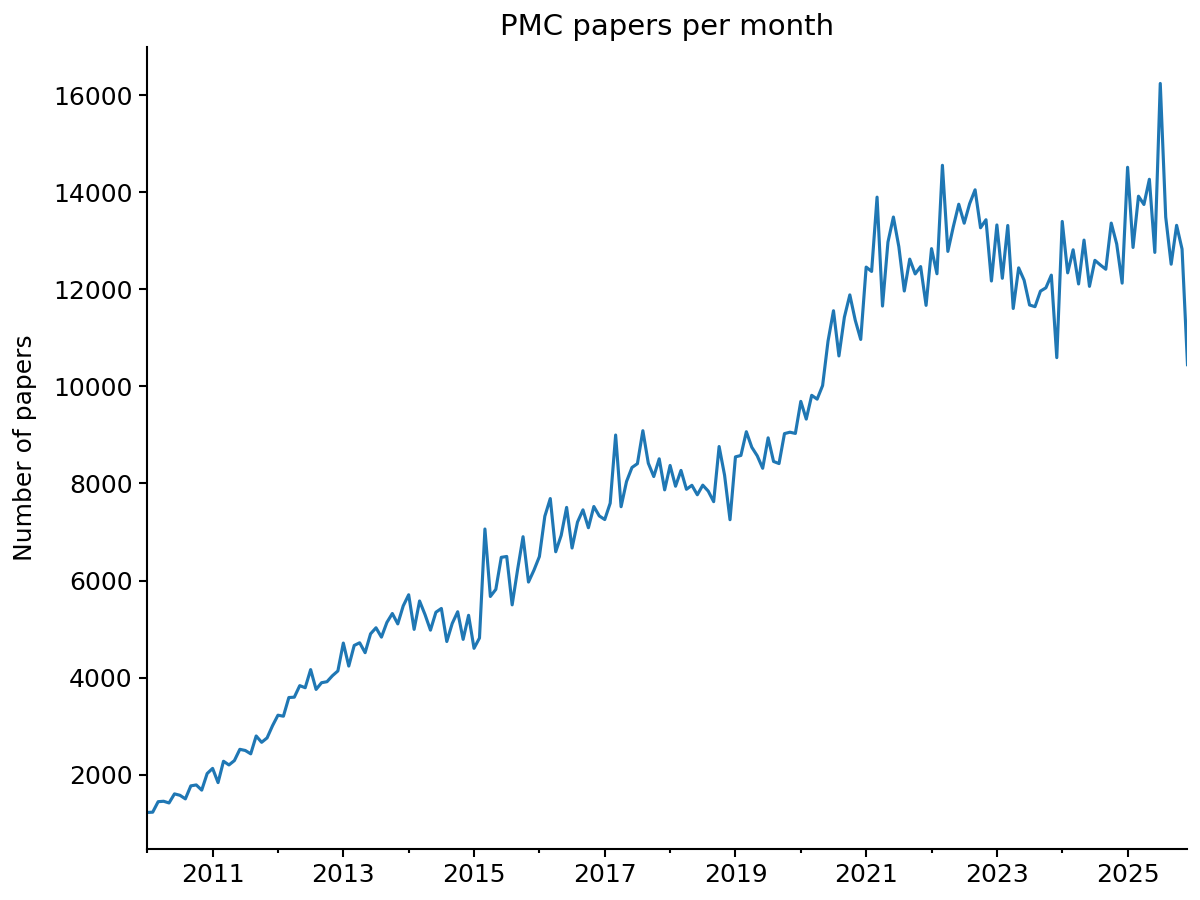
\includegraphics[width=0.7\linewidth]{../results/plots/baseline_2026-01-23/papers_per_month.png}
    \caption{}
    \label{fig:papercount}
\end{figure}
\emph{Pubmed Central}
\\
Pubmed Central (PMC) is a collection of open-access biomedical literature curated by the U.S. National Institutes of Health's National Library of Medicine \cite{pmc}. 
It provides machine-readable versions of the articles in XML format, which can be accessed individually or downloaded in bulk.
There are three open-access subsets available for bulk download with different licensing: commercial, non-commercial and other.
The latter set includes non-machine readable licenses and was therefore not used.
PMC publishes a baseline twice a year containing all papers in the collection up to shortly before the baseline's release date. 
Incremental updates are published daily in separate files.
When a new baseline is released, the previous baseline and all incremental files are replaced.
Here, we used the baseline published on January 23, 2026 containing papers dated December 31, 2025 and before.\footnote{Since work on this thesis started earlier, initial analyses used the previous baseline released June 26, 2025. These were repeated with the January 2026 baseline, so that everything reported here is based on the newer baseline}
The daily updates published after the baseline were not considered.
\\\\
\emph{XML parsing}
\\
From the XML files in the baseline, each corresponding to one paper, the following information was extracted:
\begin{itemize}
    \item Article type: specifies whether the article is a research paper, a review, a comment, etc.
    \item Date
    \item Language: only specified for a minority of papers, but is inferred later during preprocessing 
    \item Country
    \item PMC-ID: unique identifier for every paper in PMC
    \item PMID: unique identifier for PubMed, not available for every paper in PMC
    \item Journal name
    \item Title
    \item Abstract
    \item Sections
    \item Section titles
\end{itemize}
The sections and section titles are parsed from the main body of the XML file.
In general, individual sections are tagged as sec and assigned a title.
This is important for being able to compare different sections with each other, for which we need as many papers as possible with similar sections.
However, since there is no standardized format for the files, some sections are untitled or there are no section tags at all.
In particular, many files have section names for all sections except the Introduction, or don't embed the Introduction in a separate section tag. 
Therefore, if a file has more sections than section titles, and the first section is unnamed, it is assumed to be the Introduction.
Any other untitled sections are discarded.
Similarly, if there is text at the beginning of the body outside of a sec tag, it is assumed to be the introduction. 
This heuristic is not ideal, because the unnamed text contains abbreviations or keywords instead of the introduction in some cases, but since the Introduction is among the sections this study wants to focus on, it strongly increases the number of usable papers.
\\\\
\emph{Preprocessing}
\\
While some XML files specify the paper's language, this is not the case for the majority.
Since the focus here is on English text, we determine each paper's language using polyglot's detector module.
Every non-English paper is discarded.
The dates of each paper are standardized to DD-MM-YYYY format. 
Some entries only specify the month (e.g. "Feb 2025") or season of the year (e.g. "Fall 2025"), in which case the first of the month or start of the (meteorological) season are used as dates.
Papers without date are removed.
Since we want to compare LLM-use across different sections, it is important to have as many papers with comparable section structure as possible.
To achieve this, in a first step the section names were manually standardized by collecting the most frequent section names and mapping them to their standardized version.
For example, \emph{experimental results}, \emph{findings} and \emph{main results} would be mapped to \emph{results}.
If a paper has multiple sections with the same standardized title, they are concatenated.
For example, \emph{data} and \emph{experimental methods} would first both be renamed as \emph{methods} and then combined into a single \emph{methods} section.
Originally, we planned to investigate different article types and article structures, but in the end we focused only on research articles that have exactly the sections Introduction, Methods, Results, and Discussion, since papers with this article structure were the majority in the dataset.
Conversely, all papers with article types other than \emph{research-article} or with more, fewer or different sections were discarded.
Finally, all sections, including the abstract, were required to have a length of at least 250 characters.
These preprocessing steps reduce the dataset from 7,125,722 to 1,602,404 papers, 1,194,287 of which are dated 2017 or later.
\\
The use of PMC, granting us access to the whole paper, enables an extension on \cite{Kobak2025} in two regards: First, we can compare LLM-usage in the abstract to LLM-usage in the entire body of the paper, and second, we can compare different sections within the body with each other.
For this purpose, all of the analyses detailed in the following subsections were performed on the abstract, the introduction, the methods, the results and discussion of the paper, as well as the full paper, which refers to the four sections from the body without the abstract.

\subsection{Excess Frequency and LLM-use lower bound estimates}

\begin{figure}[htbp]
    \centering
    \begin{minipage}[t]{0.48\textwidth}
        \centering
        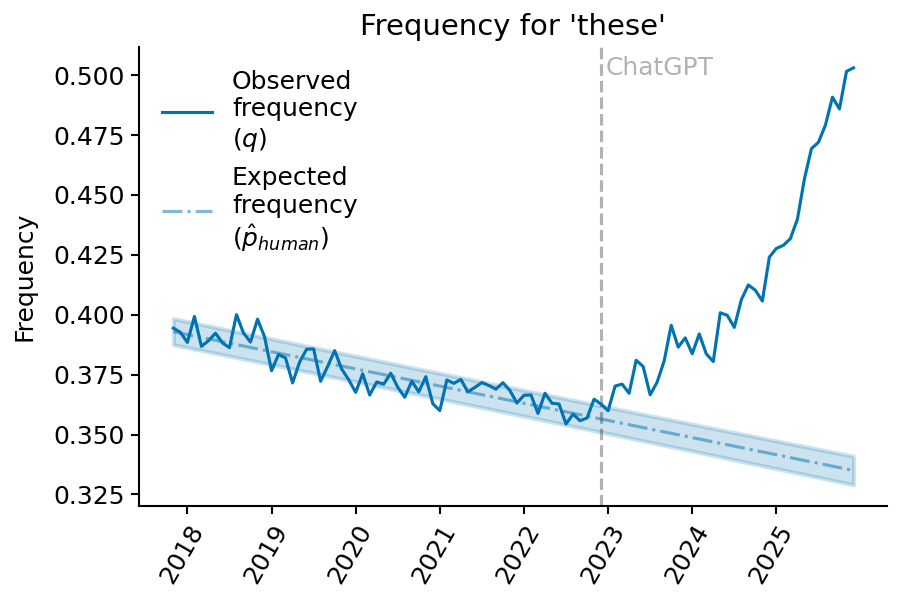
\includegraphics[width=\linewidth]{../results/plots/baseline_2026-01-23/research-article_aimrd_f/these_freqs_time.png}
    \end{minipage}
    \hfill
    \begin{minipage}[t]{0.48\textwidth}
        \centering
        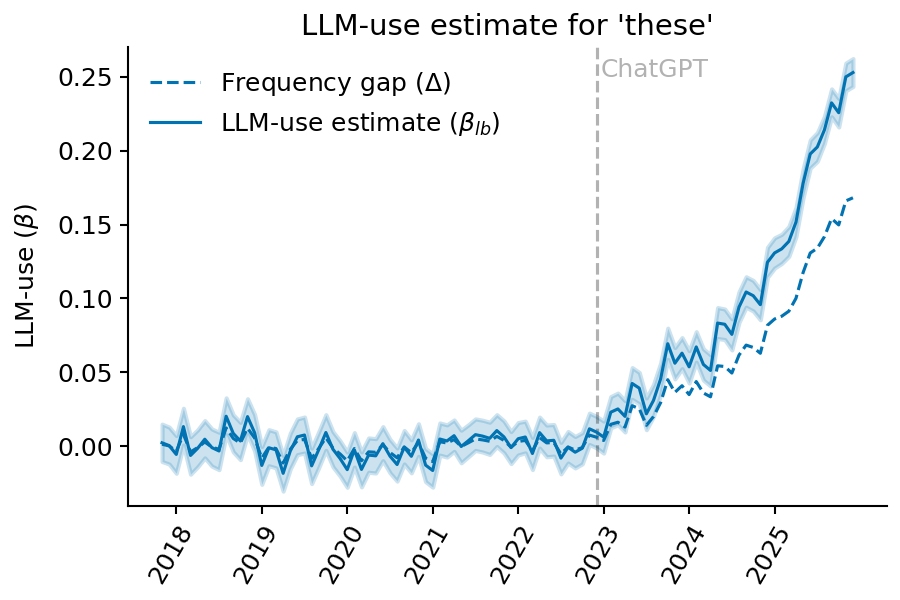
\includegraphics[width=\linewidth]{../results/plots/baseline_2026-01-23/research-article_aimrd_f/these_usage_time.png}
    \end{minipage}
    \caption{Shared caption describing both images}
    \label{fig:two_images}
\end{figure}
Excess frequency, referring to the difference between the observed and predicted frequencies for some word $w$, can be thought of as an intuitive lower bound for LLM use.
To compute it, we first determine the observed frequency of $w$.
We use sklearn's binary CountVectorizer to count the number of papers in each month or year in which $w$ occurs.
Because it is a binary count, it doesn't matter how often $w$ appears in each paper.
The vectorizer only considers words with 4 or more letters, all of which must be part of the English alphabet.
When counting word occurrence, lemmatization is an important consideration: one has to determine whether to treat different inflections of $w$ as the same or as individual words.
With lemmatization, it makes no difference if a paper contains \emph{delves}, \emph{delved} or \emph{delving}, they are all treated as an instance of \emph{delve}.
It is not immediately clear if lemmatization is helpful in this use-case.
We know from previous studies that LLMs prefer certain words.
This could imply that LLMs use all inflections of a word at a higher frequency, or that it has a strong preference for that word in a specific grammatical context (e.g. third-person singular), while using every other inflection at the same frequency in which they occur in human-written text.
As will be detailed in Section \ref{subsec:wordlist}, for the overall LLM-usage estimates, this does not matter. 
For the plots showing results for individual words, such as Figure, all word variants are included in the counts.
The frequencies are computed by dividing the monthly or yearly counts by the total number of papers in each respective time frame.
On a conceptual level, the observed frequencies $q$ are an estimate for the probability of a positive outcome in the Bernoulli trial of whether a word is present in some paper.
For dates prior to the release of ChatGPT in November 2022, marking the beginning of easily accessible LLMs, $q$ corresponds to the frequency of a word in human-written text, $p_{human}$.
After the widespread availability of Chatbots, the observed word frequency can be thought of as the product of a mixture distribution between the probability of a word to appear in human-authored and LLM-assisted text, respectively: 
\begin{equation}
    q = 
    \begin{cases}
        p_{human} & \text{for papers before 11-2022}\\
        (1-\beta) \cdot p_{human} + \beta \cdot p_{LLM} & \text{for papers after 11-2022}\\
    \end{cases}
\end{equation}
The mixture component $\beta$ in the lower case indicates the proportion of papers that were written with the help of LLMs.
We can transform this equation to obtain an expression for $\beta$:

\begin{equation}\label{eq:beta}
\begin{split}
    q &= (1-\beta) \cdot p_{human} + \beta \cdot p_{LLM}\\
    \beta \cdot (p_{LLM}-p_{human}) &= q -  p_{human}\\
    \beta &= \frac{q -  p_{human}}{p_{LLM}-p_{human}}
\end{split}
\end{equation}
\\
While $p_{human}$ can be estimated by the observed $q$ in the time span before November 2022, there is no direct way to do so after the release of ChatGPT.
However, if we assume that human usage of words follows linear trends and is independent of LLM-use, we can use the values before 2022 to model $\hph$ using linear regression.
Since we are interested in both the monthly and yearly trends, we fit the regression either on the five yearly frequency values from 2018 to (including) 2022, or on the 60 monthly frequencies from November 2017 to October 2022.
For the yearly data we include 2022 in the train set because, considering the time it takes to write a paper, and the time it took the new technology to gain traction, it is unlikely that many papers published in December 2022 were written with the help of LLMs.
Replacing the unknown $p_{human}$ with the estimate $\hph$ in equation \ref{eq:beta}, one issue remains: there is no direct way to estimate $p_{LLM}$ from the observed frequencies.
The others solve this problem by using ground-truth LLM-generated text to determine $p_{LLM}$.
Here, we choose a different approach by determining a lower bound for $\beta$ that doesn't rely on $p_{LLM}$:
\begin{equation}\label{eq:delta}
    \begin{split}
        \beta &= \frac{q -  \hph}{p_{LLM}-\hph}\\
        \beta &\ge q - \hph =\Delta
    \end{split}
\end{equation}
This is the excess frequency measure introduced by \cite{Kobak2025} and denoted $\Delta$.
Intuitively, if a word appears in $70\%$ of papers in 2025, but we predict humans to use this word in only $60\%$ of instances, the $10\%$ gap must be accounted for as having been written by LLMs. 
Note that this metric will lead to a strong under-estimation of the actual LLM usage, because a human-use frequency of $60\%$ will only translate to $60\%$ of observed use, if all texts in the sample are in fact written by humans ($\beta=0$).
In reality, some papers were written with the help of LLMs, such that the fraction of word-occurrence that can be explained by human usage is not $60\%$ of all papers, but $60\%$ of the papers with human authorship.
A stronger lower bound, denoted $\hbet$ is also possible:
\begin{equation}\label{eq:beta_hat}
    \begin{split}
        \beta &= \frac{q -  \hph}{p_{LLM}-\hph}\\
        \beta &\ge \frac{q -  \hph}{1-\hph} = \hbet
    \end{split}
\end{equation}
In dividing by $1-\hph$, this lower bound readjusts the estimate by focusing only on the fraction of papers for which no human use of the word is to be expected.
In the above example with $p_{human}=60\%$ and excess frequency of $\Delta=10\%$, $1-\hph=40\%$ of papers wouldn't contain the word if there were no LLM-authored texts, but only $1-q=30\%$ actually don't, so the remaining $\frac{10\%}{40\%}=25\%$ must be LLM-authored.  

\begin{figure}[htbp]
    \centering
    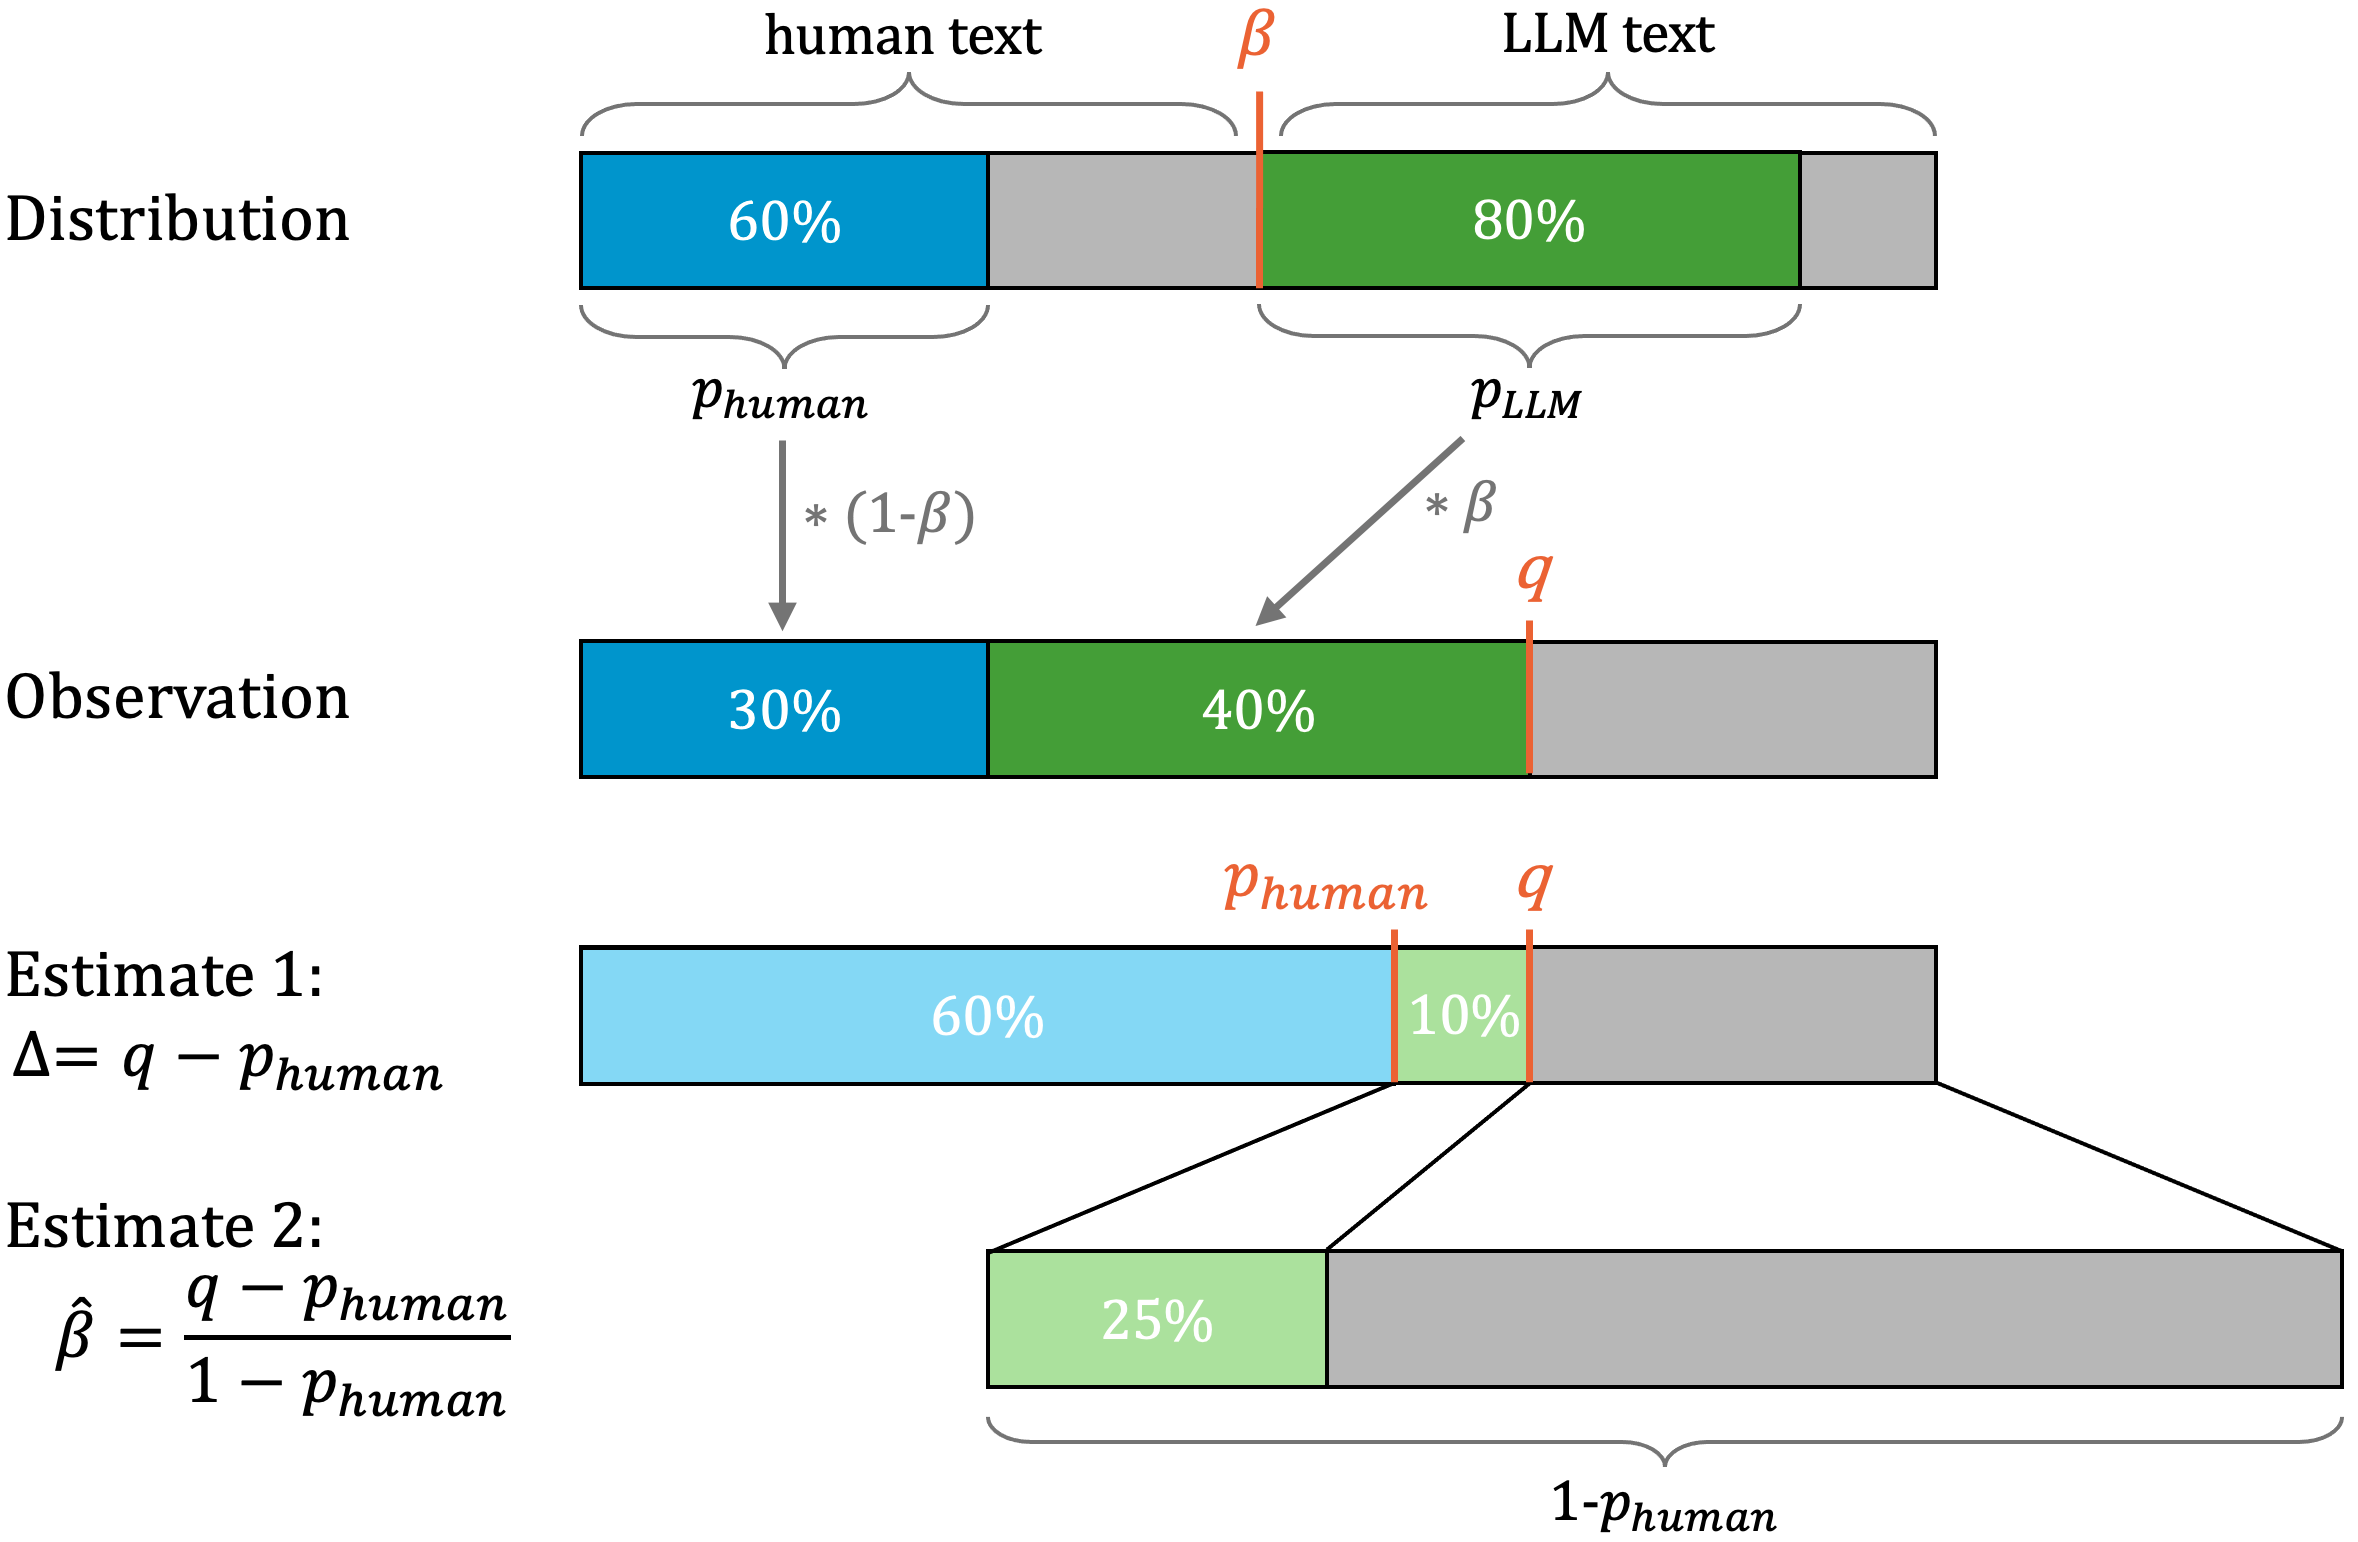
\includegraphics[width=0.7\linewidth]{../results/plots/misc/intuition_estimate_v2.png}
    \caption{}
    \label{fig:intution_estimates}
\end{figure}



\subsection{Grouped word frequencies}\label{subsec:wordlist}
\begin{figure}[htbp]
    \centering

    \begin{minipage}[t]{0.48\textwidth}
        \centering
        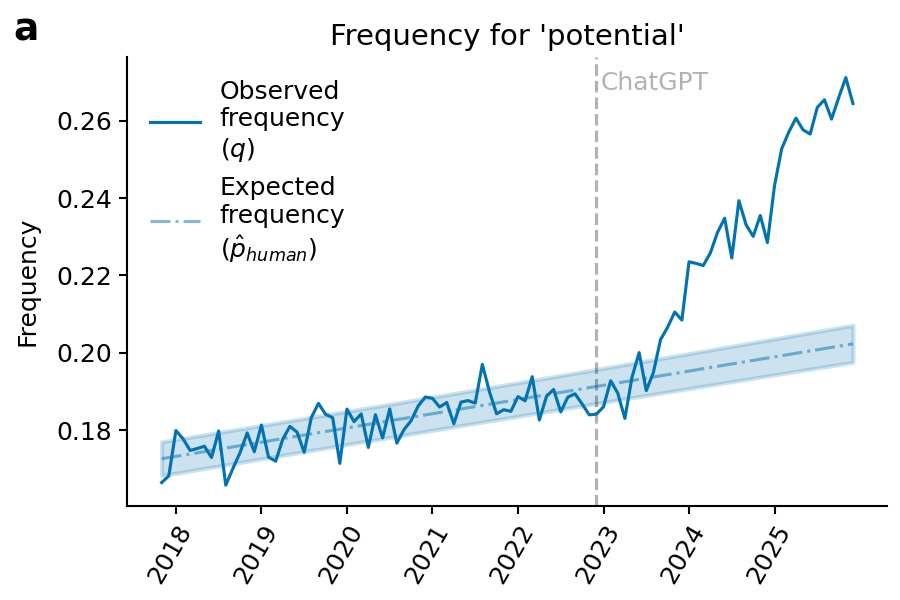
\includegraphics[width=\linewidth]{../results/plots/baseline_2026-01-23/research-article_aimrd_f/potential_freqs_time.png}
    \end{minipage}
    \hfill
    \begin{minipage}[t]{0.48\textwidth}
        \centering
        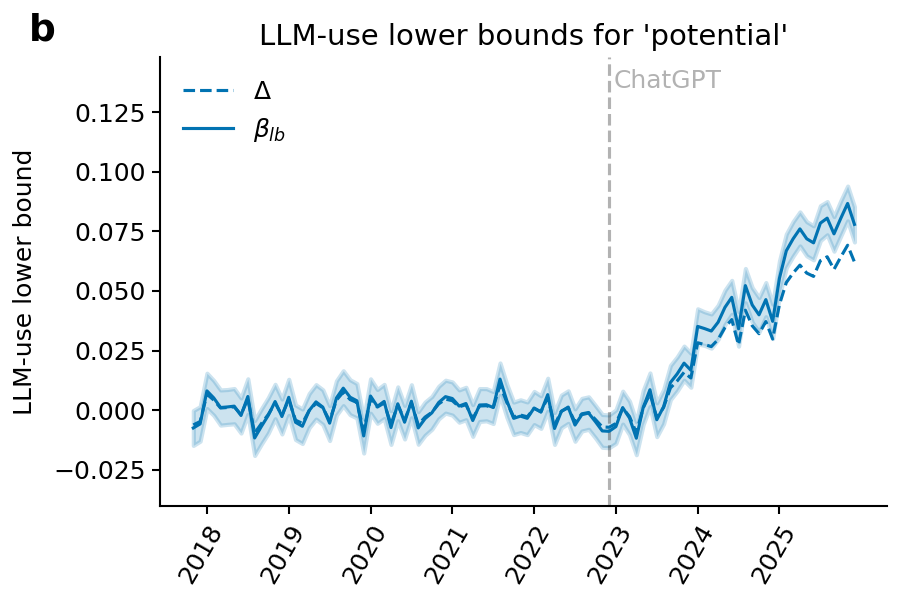
\includegraphics[width=\linewidth]{../results/plots/baseline_2026-01-23/research-article_aimrd_f/potential_usage_time.png}
    \end{minipage}

    \medskip

    \begin{minipage}[t]{0.48\textwidth}
        \centering
        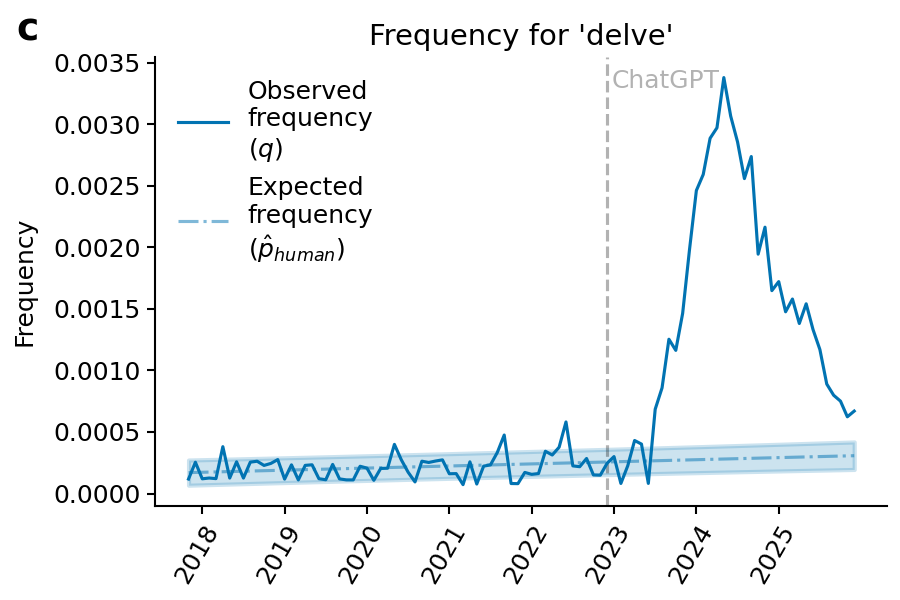
\includegraphics[width=\linewidth]{../results/plots/baseline_2026-01-23/research-article_aimrd_f/delve_freqs_time.png}
    \end{minipage}
    \hfill
    \begin{minipage}[t]{0.48\textwidth}
        \centering
        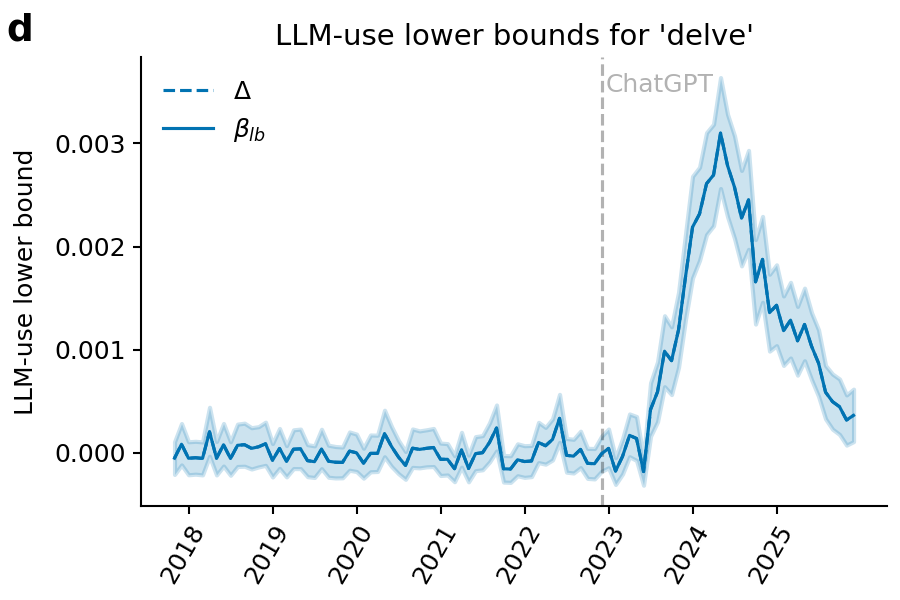
\includegraphics[width=\linewidth]{../results/plots/baseline_2026-01-23/research-article_aimrd_f/delve_usage_time.png}
    \end{minipage}

    \caption{Fix title for delve estimates!}
    \label{fig:four_images}
\end{figure}

While single words are useful to illustrate the concept of excess frequency, they are suboptimal as a basis for an accurate estimate of overall LLM-use.
The reason for this is obvious: while LLMs might use a word such as ``potentially'' at a higher frequency than humans would, ``potentially'' doesn't fit in every context so there will potentially be a lot of LLM texts not containing it.
Also, the observed frequencies of some words might be unreliable.
The word ``delve'', used as the titular example of excess vocabulary in \cite{Kobak2025}, has experienced a sharp decline in popularity starting around mid-2024, when it was widely reported as an example of ``LLM-speak''.
Many authors have thus moved to using word lists as markers. 
The method of computing the frequencies doesn't change, but instead of counting in how many papers a single word appears, we count in how many papers at least one of the words in the list appears.
The most systematic way to create a list of words indicative of LLM-use is to use a data-driven approach, which doesn't require a manually selected list.
\\\\
\emph{Excess words for 2024 PubMed}
\\
\cite{Kobak2025} determine the excess words for 2024 by computing the frequency gap and the frequency ratio for each word in their dataset.
The frequency gap is the same metric as $\Delta$ in Equation \ref{eq:delta}, although they only use the yearly frequencies of 2021 and 2022 to predict $\hph$.
The frequency ratio is computed as $\frac{q}{\hph}$.
An excess word is defined as any word with frequency gap or frequency ratio above a certain threshold.
The thresholds were chosen in such a way that the majority of words in texts from the years 2012 - 2023 were excluded
(The gaps for previous years were also computed by comparing observed values to $\hph$ computed based on two and three years prior).
Using both metrics as inclusion criteria serves to increase the number of excess words.
For instance, a word whose usage increases from 0.0001 to 0.001 will have a relatively small gap but a large ratio, while a word whose prior frequency of 0.3 rises to 0.4 has a large gap with a relatively small ratio. 
Both changes mark a notable difference in usage and should therefore be candidates for marker words.
All words above the threshold were then manually annotated as \emph{style words} or \emph{content words}.
\emph{Content words} are all words related to the research topic of a certain paper. 
Their excess use can be attributed to new inventions or research trends.
Examples include ``RNN'' in 2018, ``Covid'' in 2020, and ``ChatGPT'' in 2024.
\emph{Style words}, on the other hand, are not related to research topics and could be found in any discipline: ``these'', ``potentially'', ``delve'', etc.
Excess words of 2024 were defined as all style words with frequency gap or ratio gap above the respective thresholds.
This resulted in a list of 379 words, which can be found in the Appendix \ref{ap:wordlist}.
\\\\
\emph{Optimal word lists}
\\
The excess word list can be used to create the optimal list of marker words to detect LLM-use.
It might be counter-intuitive to not just use the whole list: if any of the words can act as a marker for LLM-use, then using as many words as possible should yield the most accurate result.
However, one has to keep in mind that all excess words also appear in human-written text.
If there are too many words in the list, their cumulative frequency will be close to 1 even for $p_{human}$.
For \cite{Kobak2025}, who use the frequency gap $\Delta$ as their LLM-use estimate, this is suboptimal because the closer $\hph$ is to 1, the smaller the potential gap.
When using $\hbet$ as the metric, the best estimate would be achieved by getting $p_{LLM}$ as close to 1 as possible, which would in turn move $\hbet$ closer to the true value $\beta$.
While $p_{LLM}$ isn't observable, it can be manipulated by increasing the number of words in the excess list.
However, this also includes the caveat that $\hph$ must remain smaller than 1, otherwise, Equation \ref{eq:beta_hat} yields division by zero.
This means that for both estimates, $\Delta$ and $\hbet$, a subset of the 2024 excess words needs to be determined.
Because brute-forcing the decision on an optimal list by trying all possible combinations is not feasible, \cite{Kobak2025} sorted the excess words by their individual frequencies in 2024 (lowest to highest), and then used different cutoff values to create subsets of all words whose individual frequencies were below the cutoff. 
Each resulting list was used to compute the LLM-use estimate $\Delta$ and the highest $\Delta$ was used as the final estimate.
\\\\
\emph{Adaptation to PMC data}
%comment: include graph of excess words for one section? also include the paper composition?
Initially, we planned to repeat the procedure of finding excess words for the PMC dataset.
This turned out to be non-feasible, because the length of the full papers, as opposed to only abstracts, lead to a huge number of excess words, which would all have to be manually annotated to filter them for style words.
Instead, we used the previous study's 2024 excess word list.
This is permissible because, first, PMC is a subset of the PubMed data used in \cite{Kobak2025}, so the domain is similar, and second, the point of using style words is to have marker words that are domain-independent.
(Although it is likely that when searching for excess words in a different domain, such as news articles, the resulting list would be somewhat different).
The 2024 excess word list is not lemmatized, so that ``delving'' and ``delves'' are treated as different words.
Since we are not interested in the excess words on a semantic level and use them only as indicator of LLM use, it does not matter if two words on the list are variations of the same verb, or if a third variation of the verb is not included.
To get the optimal list for each section, we sort the 2024 excess words by their individual frequency in 2024.
This leads to a somewhat different order for each section.
Like in the previous work, we then use different cutoff values to create subsets of excess words, which serve as a basis for computing the LLM-use estimate $\hbet$.
We started with x cutoffs spaced evenly on a log-scale between 0 and 1 and later added intermediate values in the high-interest region around the maximum, resulting in y cutoffs.
Initially, we used the same approach as above to select the maximum $\hbet$-value as the estimate.
However, in some cases, the maximum was at one of the highest cutoff value, leading to nearly the full excess word list being used for the estimate.
This results in values for $q$ and $\hph$ that are extremely close to 1, sometimes with $\hph$ being larger than $q$, which contradicts the assumption $p_{human} < p_{LLM}$.
As a consequence, both numerator and denominator of the fraction $\frac{q - \hph}{1-\hph}$ are very close to 0, which can lead to unstable behavior.
To prevent this, any cutoff that leads to estimates of $\hph \ge 0.999$ was excluded as candidate for creating optimal excess word lists.
%comment: check this number and include plot that shows oscillation of estimates that go too close to 1
\\
The optimization was performed on yearly frequency data separately.
This means that the optimal cutoff for 2024 could be different to that of 2025.
For the main analysis, the optimal cutoff values for 2025 were used for all time points to simplify procedure and have more easily comparable results.
Notably, the main analysis was performed on monthly data with the word lists optimized for the year 2025, instead of optimizing each month individually, for simplicity.
A possible approach with optimizing on monthly intervals of the data would be to take the majority optimum as the list for all estimates.
The end result would be the same: Some time intervals would be estimated with the optimal word list, while others wouldn't.
\\
To better judge the reliability of the estimates, we computed the standard error and performed sanity checks using simulated frequency data.

\subsection{Method validation}
\emph{Standard error for LLM-use estimates}
Since the LLM-use estimate $\hbet=\frac{q -  \hph}{1-\hph}$ depends on $\hph$ and $q$, we first need to determine their respective errors, before propagating them to obtain the error for $\hbet$.
We conceptualize $q$ as the maximum likelihood estimate (MLE) for the binomial probability of a word from the excess word list to appear in a paper.
As such, the MLE's variance is $SE_q^2=\frac{q(1-q)}{n}$, with $n$ as the number of papers in the current month or year.
$\hph$ is the regression estimate of a binomial probability. 
Since $\hph$ is not an empirical estimate, the binomal MLE variance doesn't apply and we focus on the regression variance.
Technically, the data points that the regression was trained on are empirical estimates (since training was done on $q$ values in the time span before the release of ChatGPT).
To factor in this binomial maximum likelihood uncertainty, it should be included in the regression formula.
However, because the MLE variance is very small due to the large number of papers each month, this was omitted for simplicity.
The regression variance for design matrix $X$ (including only points on which the regression is fit, corresponding to the time before the release of ChatGPT), predictor matrix $x$ (including all points that are to be predicted, including pre- and post-ChatGPT frequencies) and response vector $y$ is computed with the following formula:
\begin{equation}
    SE_{\hph}^2= \hat{\sigma}^2 x(X^TX)^{-1}x^T + \hat{\sigma^2}
\end{equation}
with $\hat{b}=(X^TX)^{-1}X^Ty$ as the estimated regression coefficients\footnote{As per common convention, the estimated regression coefficients are normally denoted $\hbet$, which was changed to $\hat{b}$ to avoid confusion with the LLM-use estimate $\hbet$}
and $\hat{\sigma}^2=\frac{\|y-X\hat{b}\|^2}{n-2}$ the unbiased estimate of the noise variance, where $n$ refers to the number of papers, of which the number of predictors, 2, is subtracted.
$\hat{\sigma}^2x(X^TX)^{-1}x^T $ is the covariance matrix of the regression coefficients, specifying the uncertainty of the mean prediction. 
To this, an additional $\hat{\sigma}$-term is added to estimate how far the predicted values would have deviated from this mean.
\\
The variance of $\hbet$, as a nonlinear function of $q$ and $\hph$, is not trivial to determine.
We can apply the Delta method, which uses Taylor series approximation, to do so.
We assume $q$ and $\hph$ to be the means of random variables $Q$ and $P$, respectively.
First, we approximate $\hbet((Q,P))$ around the mean $\mu=(q, \hph)$ with a first-order Taylor expansion:
\begin{equation}
    \hbet((Q,P)) \approx \hbet(\mu) + \nabla\hbet(\mu)^T((Q,P)-\mu)
\end{equation}
with gradient $\nabla$ as
\begin{equation}
    \nabla \hbet(\mu)= \left[ \frac{\partial\hbet}{\partial q}, \frac{\partial\hbet}{\partial \hph}\right]^T = \left[ \frac{1}{1-\hph}, \frac{q-1}{(1-\hph)^2}\right]^T 
\end{equation}
We can use this to compute the variance of $\hbet$:
\begin{equation}
    \begin{split}
        Var(\hbet) &= Var(\hbet(\mu) + \nabla\hbet(\mu)^T((Q,P)-\mu)\\
        &= Var(\hbet(\mu) + \nabla\hbet(\mu)^T(Q,P)-\nabla\hbet(\mu)^T\mu)\\
        &= Var(\hbet(\mu)^T(Q,P))\\
        &= \nabla\hbet(\mu)^T\Sigma\nabla\hbet(\mu)
    \end{split}
\end{equation}
We assume independence of the two random variables $Q$ and $P$, so that the covariance matrix $\Sigma$ only has the diagonal entries of the estimate variances $SE_q^2$ and $SE_{\hph}^2$ derived above. 
We excluded all estimates with a standard error of $SE_{\hbet}\ge 0.025$.
%comment: the error bars don't work if p is 1 (or veryvery close to 1), because in that case, binomial error is 0
\\\\
\emph{Sanity check simulation}
\\
\begin{figure}[htbp]
    \centering
    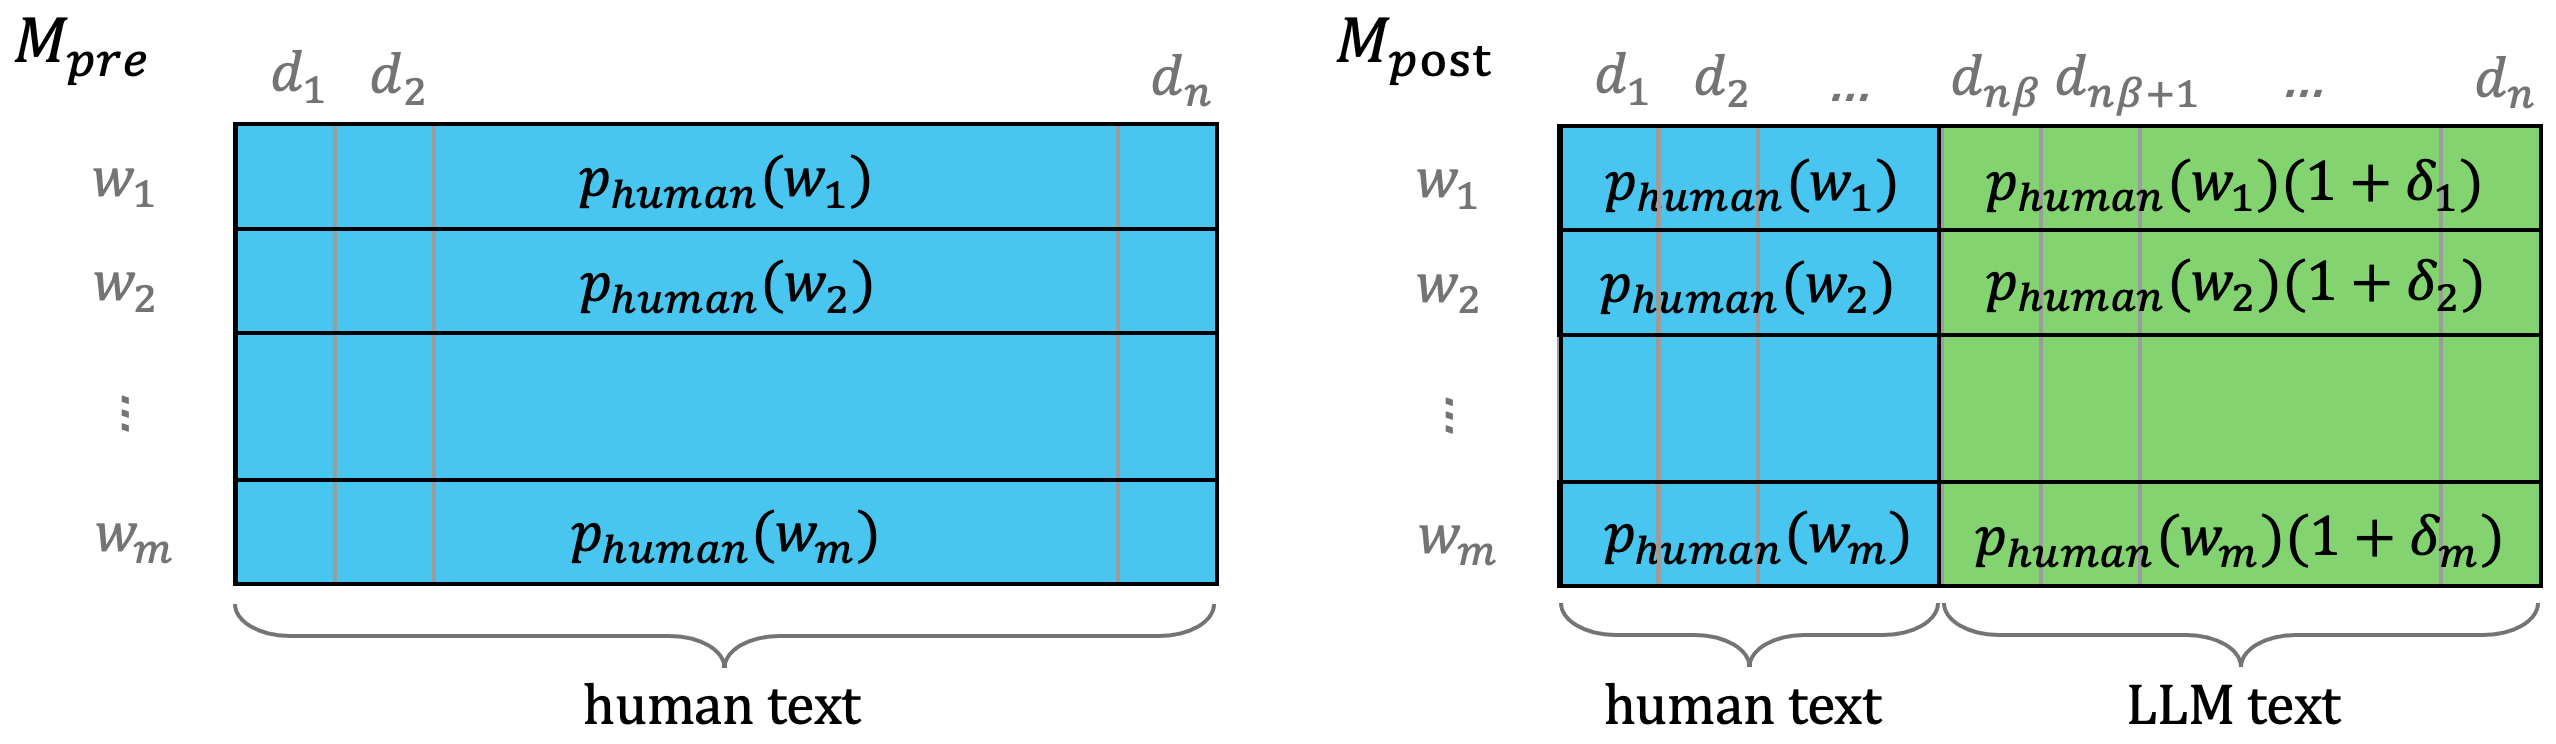
\includegraphics[width=0.9\linewidth]{../results/plots/misc/intuition_simulation_v2.png}
    \caption{Illustration of the sampling procedure for the creation of an artificial dataset to test the LLM use estimate $\hbet$ for varying levels of $\beta$}
    \label{fig:intution_simulation}
\end{figure}
To better gauge how well the procedure of finding the optimal excess word list to get the best possible lower bound works, we performed the same analysis on simulated data with known $\pl$ and $\ph$ and varying $\beta$.
We simulated data for 100,000 texts, approximating the number of papers per year in our sample.
In our simulation, there were 500 words, all of which were treated as excess words.
We created two matrices, $M_{pre}$ and $M_{post}$, each with dimensions (\emph{number of texts, number of words}), corresponding to data before and after the release of ChatGPT, respectively.
For $M_{pre}$, each word $w$ was randomly assigned a probability $\ph(w)$. 
The probabilities were sampled from a gamma distribution with shape parameter $2$ and scale parameter $0.02$.
Then, 100,000 binomial samples were drawn with $\ph(w)$ as probability of success for each word.
For $M_{post}$, a fraction of $\beta$ texts were selected as being LLM-generated.
As one of the assumptions posits that $\ph\le\pl$, the probabilities for words to occur in LLM-assisted text were sampled as $\pl(w)=\ph(w)(1+\delta)$, with $\delta \sim U(0.5,5)$.
In cases where $\ph(w)(1+\delta)>1$, $\delta$ was newly sampled until the resulting $\pl(w)$ was in the range $[0,1]$.
In the sampling process $100,000\cdot \beta$ binomial samples were drawn with probability $\pl(w)$, and $100,000\cdot (1-\beta)$ were drawn with probability $\ph(w)$.
\\
For the following analyses, the word frequencies in $M_{pre}$ was treated as analogous to $\hph$, and those in $M_{post}$ as the observed frequencies $q$.
The words in $M_{pre}$ were ordered by frequency, and excess lists were formed of words with frequencies lower than those of several different cutoffs. 
For each excess list corresponding to one of the cutoffs, the LLM-use estimates $\Delta$ and $\hbet$ were computed.
The only difference w.r.t. the procedure on the real data was during variance computation: $M_{pre}$, as opposed to $\hph$, is not the result of a regression, but, similar to $q$ the result of a binomial sampling procedure. 
Thus, the variance for frequencies based on $M_{pre}$ was computed as the variance of a binomial estimator, $Var(M_{pre}) = \frac{p(1-p)}{n}$ with $p$ the observed frequency and $n=(1-\beta)\cdot n_{texts}$.
As with the real data, we exclude cutoffs yielding frequencies $\ge0.999$ for $M_{pre}$, as well as estimates with error bars $\ge0.025$.


\subsection{Section length}
One of the goals of this project was to compare the estimated LLM-use of different sections of the paper with each other.
This might seem like an unfair comparison: When using word occurrence as LLM-marker, longer texts are at an advantage - there is simply more space for words to appear in.
[Figure here shows the different section lengths]
For example, if an LLM produced some word once every 500 words on average, it would appear in the majority of 1000-word sections, but only in about half of 250-word sections, despite all of them being written by an LLM.
Since the word counts are binary, there is no correction for section length in the estimate.
This is a further argument for using section specific word lists instead of single words.
The longer the word list, and the higher their aggregated frequency, the less likely it is for an LLM-generated text, however short, to not contain at least one of them.
However, when authors use LLMs, it is also likely that they focus their usage on specific paragraphs that they, e.g., wish to rephrase.
A longer section contains more paragraphs that might warrant re-working.
One way to address this issue is to slightly shift the question from \emph{How high is LLM-use in this section?} to \emph{How high is LLM-use in a random paragraph of this section?}
% By focusing on paragraphs instead of full sections, the section length can be controlled for. 
This was implemented by cropping each section sample to a length of 255 words, which corresponds to the median length of the abstracts.
The cropped part was placed randomly within the section by sampling a starting position ranging between the first and 255th-last words in the text.
Note that the LLM-use estimate based on the cropped sections can't be used to determine the full fraction of papers that were written with some LLM participation.
Since we are interested in identifying not only those papers that are wholly written by an LLM, using only one paragraph per section will underestimate the number of papers written with the help of LLMs, because this paragraph might not include the parts of the paper where LLMs were used. 
However, by comparing the results from the full and cropped sections, we can check whether LLMs are used universally across the entire paper or whether their use is concentrated on some paragraphs.



\subsection{Subgroup analysis}
%comment: add plot with number of paper per country (barplot for ind country counts, say 2017 to 2025, pie chart with entries "english-speaking", "non-english speaking", "unknown country")
Another point of interest is how LLM-use differs across subsets of the data.
It is, for instance, plausible to assume that majority English-speaking countries will show different usage patterns than countries where English is learned as a second language.
Likewise, there might be differences between academic disciplines, with some being quicker to adopt a new technology.
Previous studies typically reported higher usage estimates for research areas related to computer science.
To compare these categories, we repeated the experiments on different subsets of papers.
\\\\
\emph{Countries}
\\
The most salient criterion to compare countries with each other when it comes to LLM-use is their majority native language.
Since English is the de facto lingua franca of academia, one of the key capabilities of LLMs is their ability to translate or proofread text from authors uncertain of their English proficiency.
As this use-case is irrelevant for native English speakers, it stands to reason that LLM-usage would be smaller for English-speaking countries.
\\
To categorize countries into English and non-English speaking, we used the \emph{Three circles of English model}\cite{kachru1985standards}, which sorts the United States, the United Kingdom and Ireland, Australia and New Zealand, South Africa, and the majority of Canada into the ``inner circle'', where English is the native language of the majority of inhabitants and primarily used in their day-to-day lives.
All other countries were classified as non-English speaking. 
Additionally to comparing English to non-English speaking countries, we also analyzed the LLM-use of individual countries.
We selected the 18 countries with highest paper counts in the years 2017 to 2025.
The full list of countries and their respective paper counts can be found in the Appendix.
\\
We originally planned to use the excess word lists that are optimal for each section with regards to the full dataset. 
However, this lead to observations of $q=1.0$ for several years and countries (pre- and post-release of ChatGPT).
Due to time constraints, it was unfeasible to search for the optimal list for every country and section.
As a heuristic to approximate the search process, the list corresponding to the next-lower cutoff was selected.
For example, for the abstract, the optimal cutoff was $0.1$, so we selected the list corresponding to a cutoff value of $0.07$, which was the value directly preceding $0.1$.
By lowering the cutoff, we reduce the number of words in the excess word list and can thus regulate the observed frequencies.
This ``suboptimal'' cutoff also lead to problematic observations, because in many cases, $q$ was within the regression error of $\hph$, which is not ideal for any metric depending on the difference between the two.
To adjust, we moved the cutoff value one position further down, e.g. by going from $0.1$ to $0.05$ instead of $0.7$ for the abstract.
\\\\
\emph{Research disciplines}
\\
%comment same plot as for countries, maybe put in appendix? or do table instead of plot?
Papers were sorted into different research areas based on the titles of journals in which they were published in a procedure based on \cite{gonzalez2024landscape}.
The research areas are subfields of the biomedical domain, for example radiology or nursing, that were specified in \cite{gonzalez2024landscape}.
The full list of categories can be found in the Appendix.
Journals were sorted into a category via keyword search with the category titles, and were assinged no label in case of no match.
This is a relatively crude but simple approach that ignores many potential matches, e.g., the (hypothetical) \emph{Journal of Neurology} would be assigned the label ``neurology'', while the \emph{Neurological Journal} would not. 
The number of matches could be improved by using fizzy matching or manually annotating 
In assigning labels, the keyword appearing latest in the title was given precedence. 
For example, the \emph{Journal of Cancer Biochemistry} would be sorted into the ``biochemistry'' category, while \emph{The Biochemistry of Cancer} would be assigned the label ``cancer''.
This procedure resulted in 23\% of papers being labeled.
Only labels with more than 5000 papers were selected for further analysis.
Using the optimal excess word lists to compute frequencies lead to similar problems as detailed above, which is why we also used the cutoff twice removed from the optimal one.


\section{Results}\label{sec:results}
\subsection{Simulation}
%comment: these plots should ideally also include the sampling distribution (or put that in the methods?)
\begin{figure}[htbp]
    \centering
    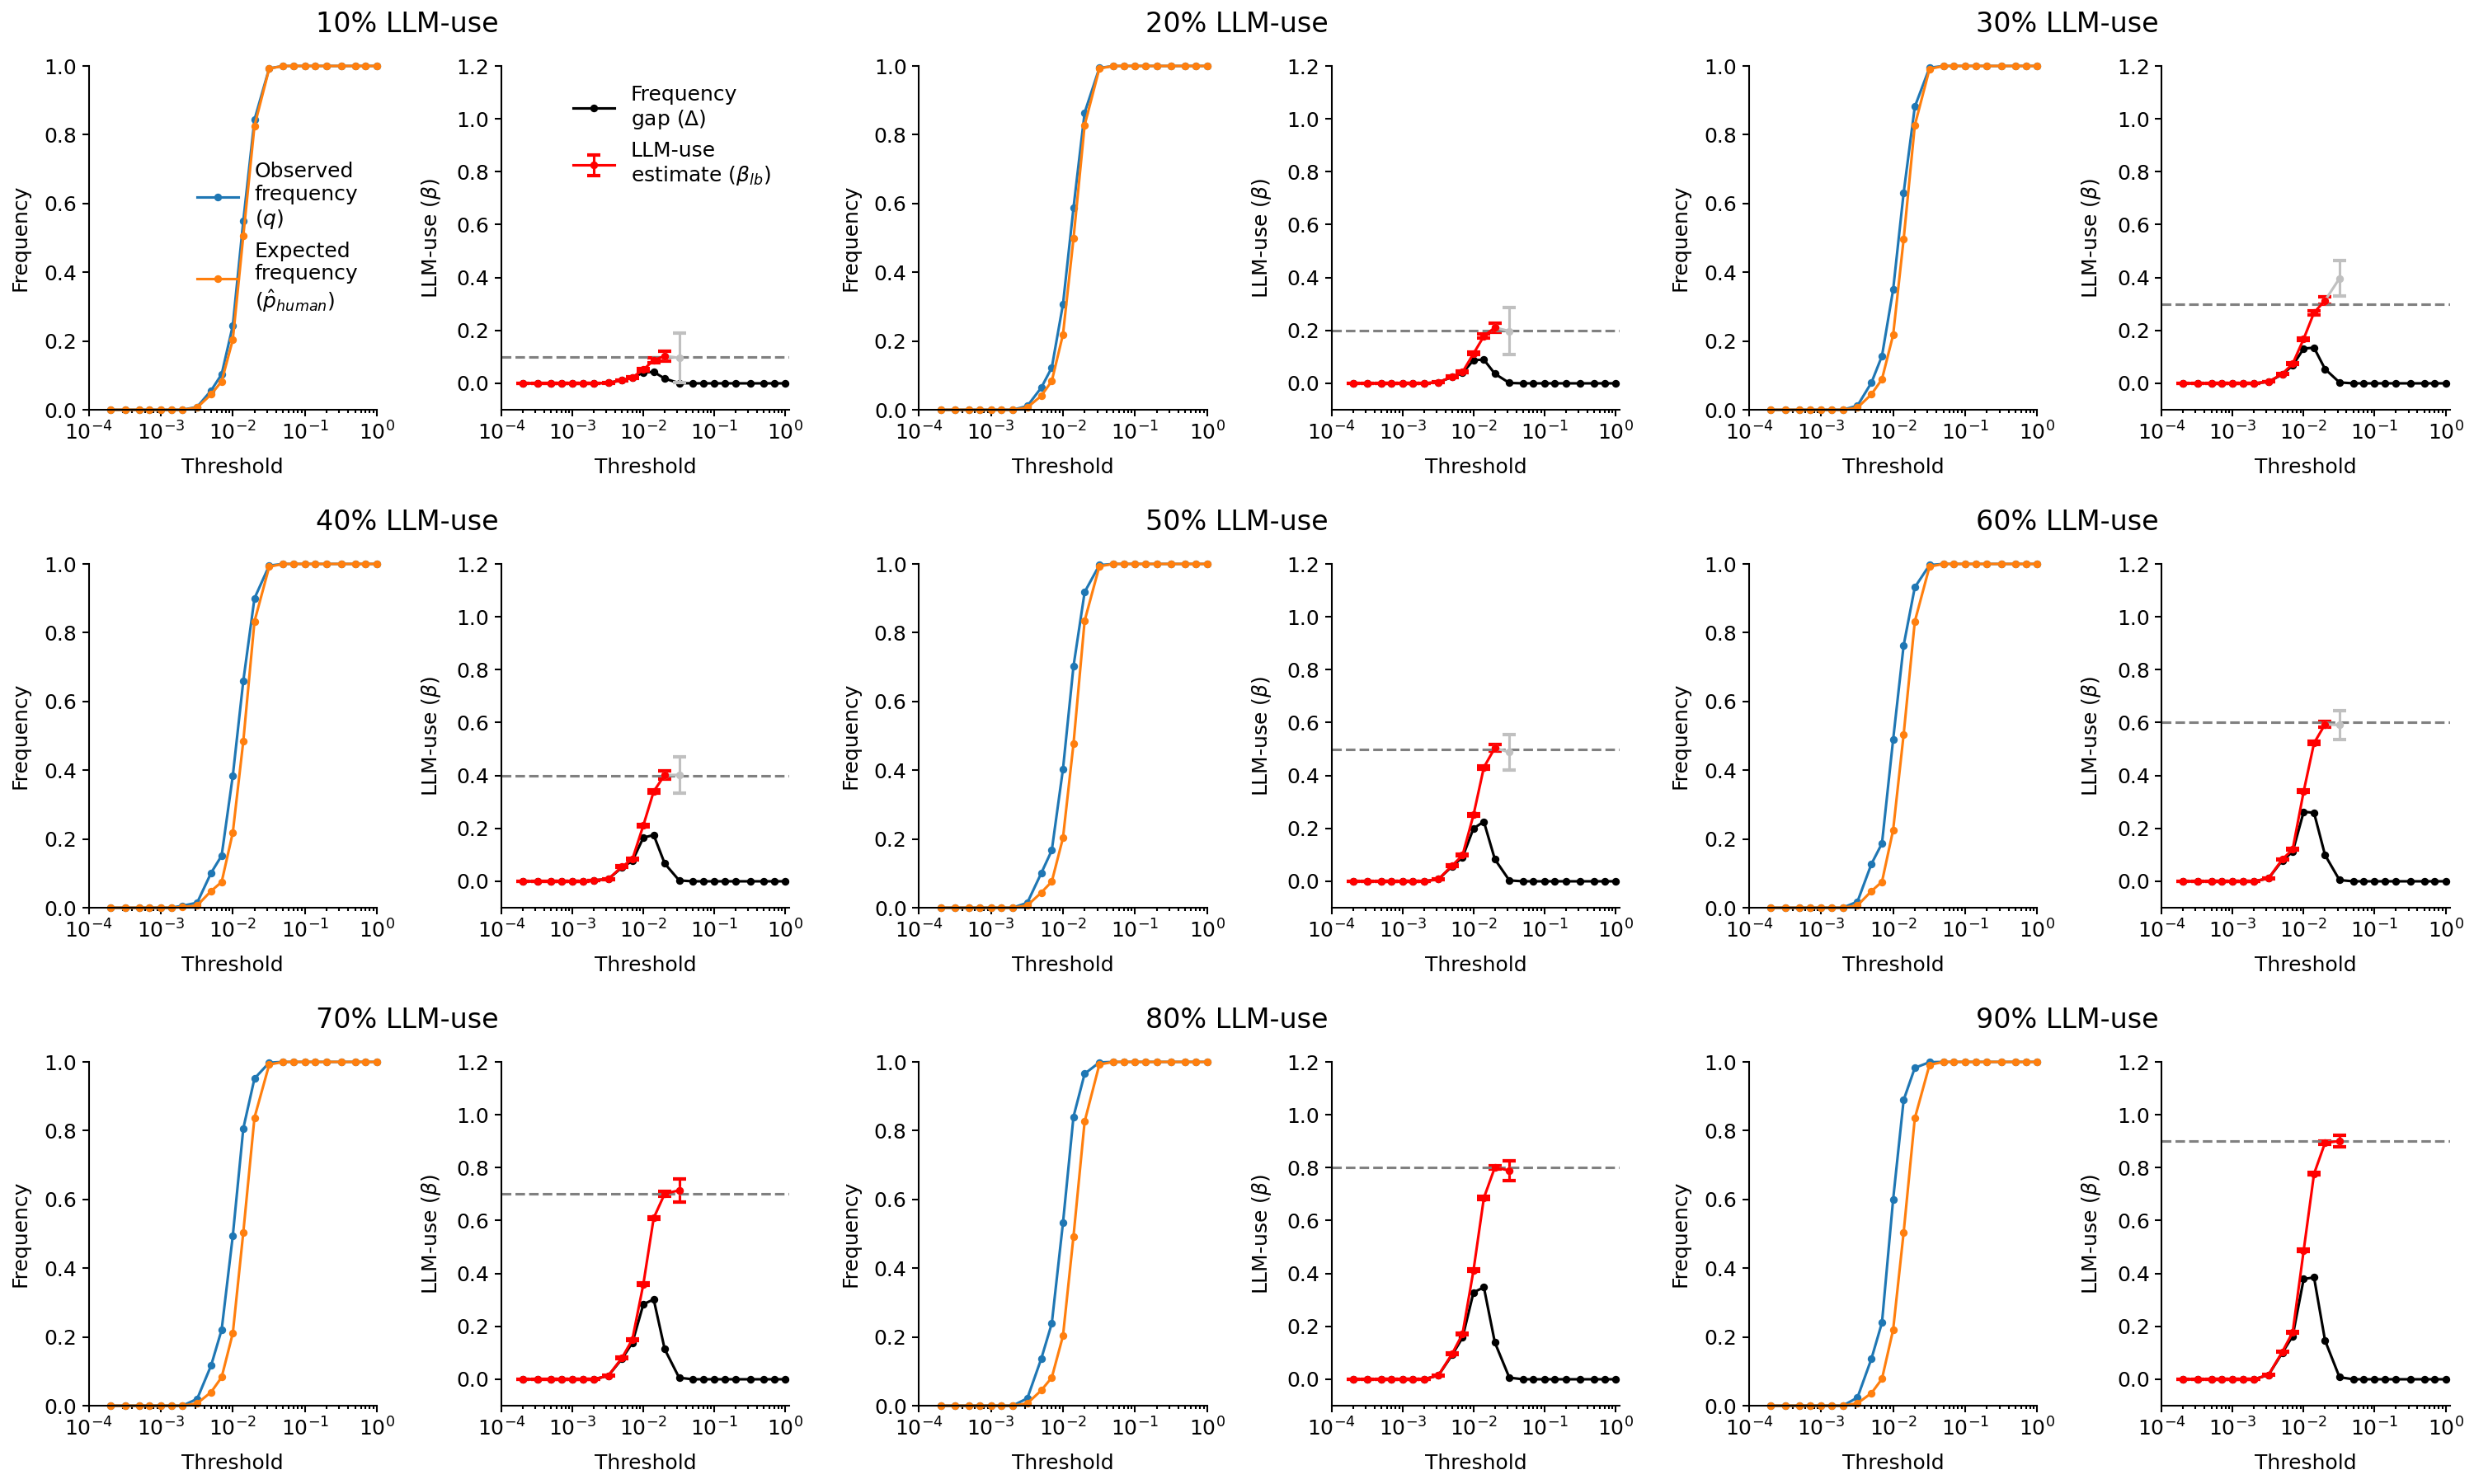
\includegraphics[width=\linewidth]{../results/plots/ground_truth_simulation/500_words.png}
    \caption{}
    \label{fig:simulation500}
\end{figure}
\begin{figure}[htbp]
    \centering
    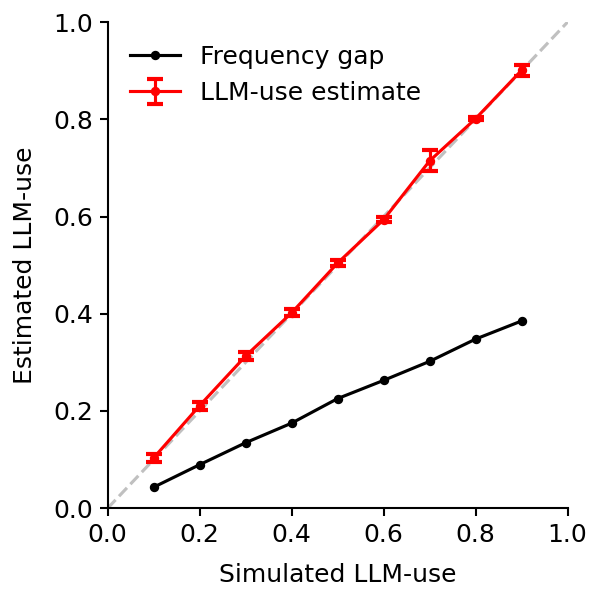
\includegraphics[width=0.5\linewidth]{../results/plots/ground_truth_simulation/500_words_overview.png}
    \caption{}
    \label{fig:simulation_overview}
\end{figure}

\subsection{Individual word estimates?}
%comment: might be interesting to include section comparison of individual words, need the plots for that
\subsection{Word list estimates}
\begin{figure}[htbp]
    \centering
    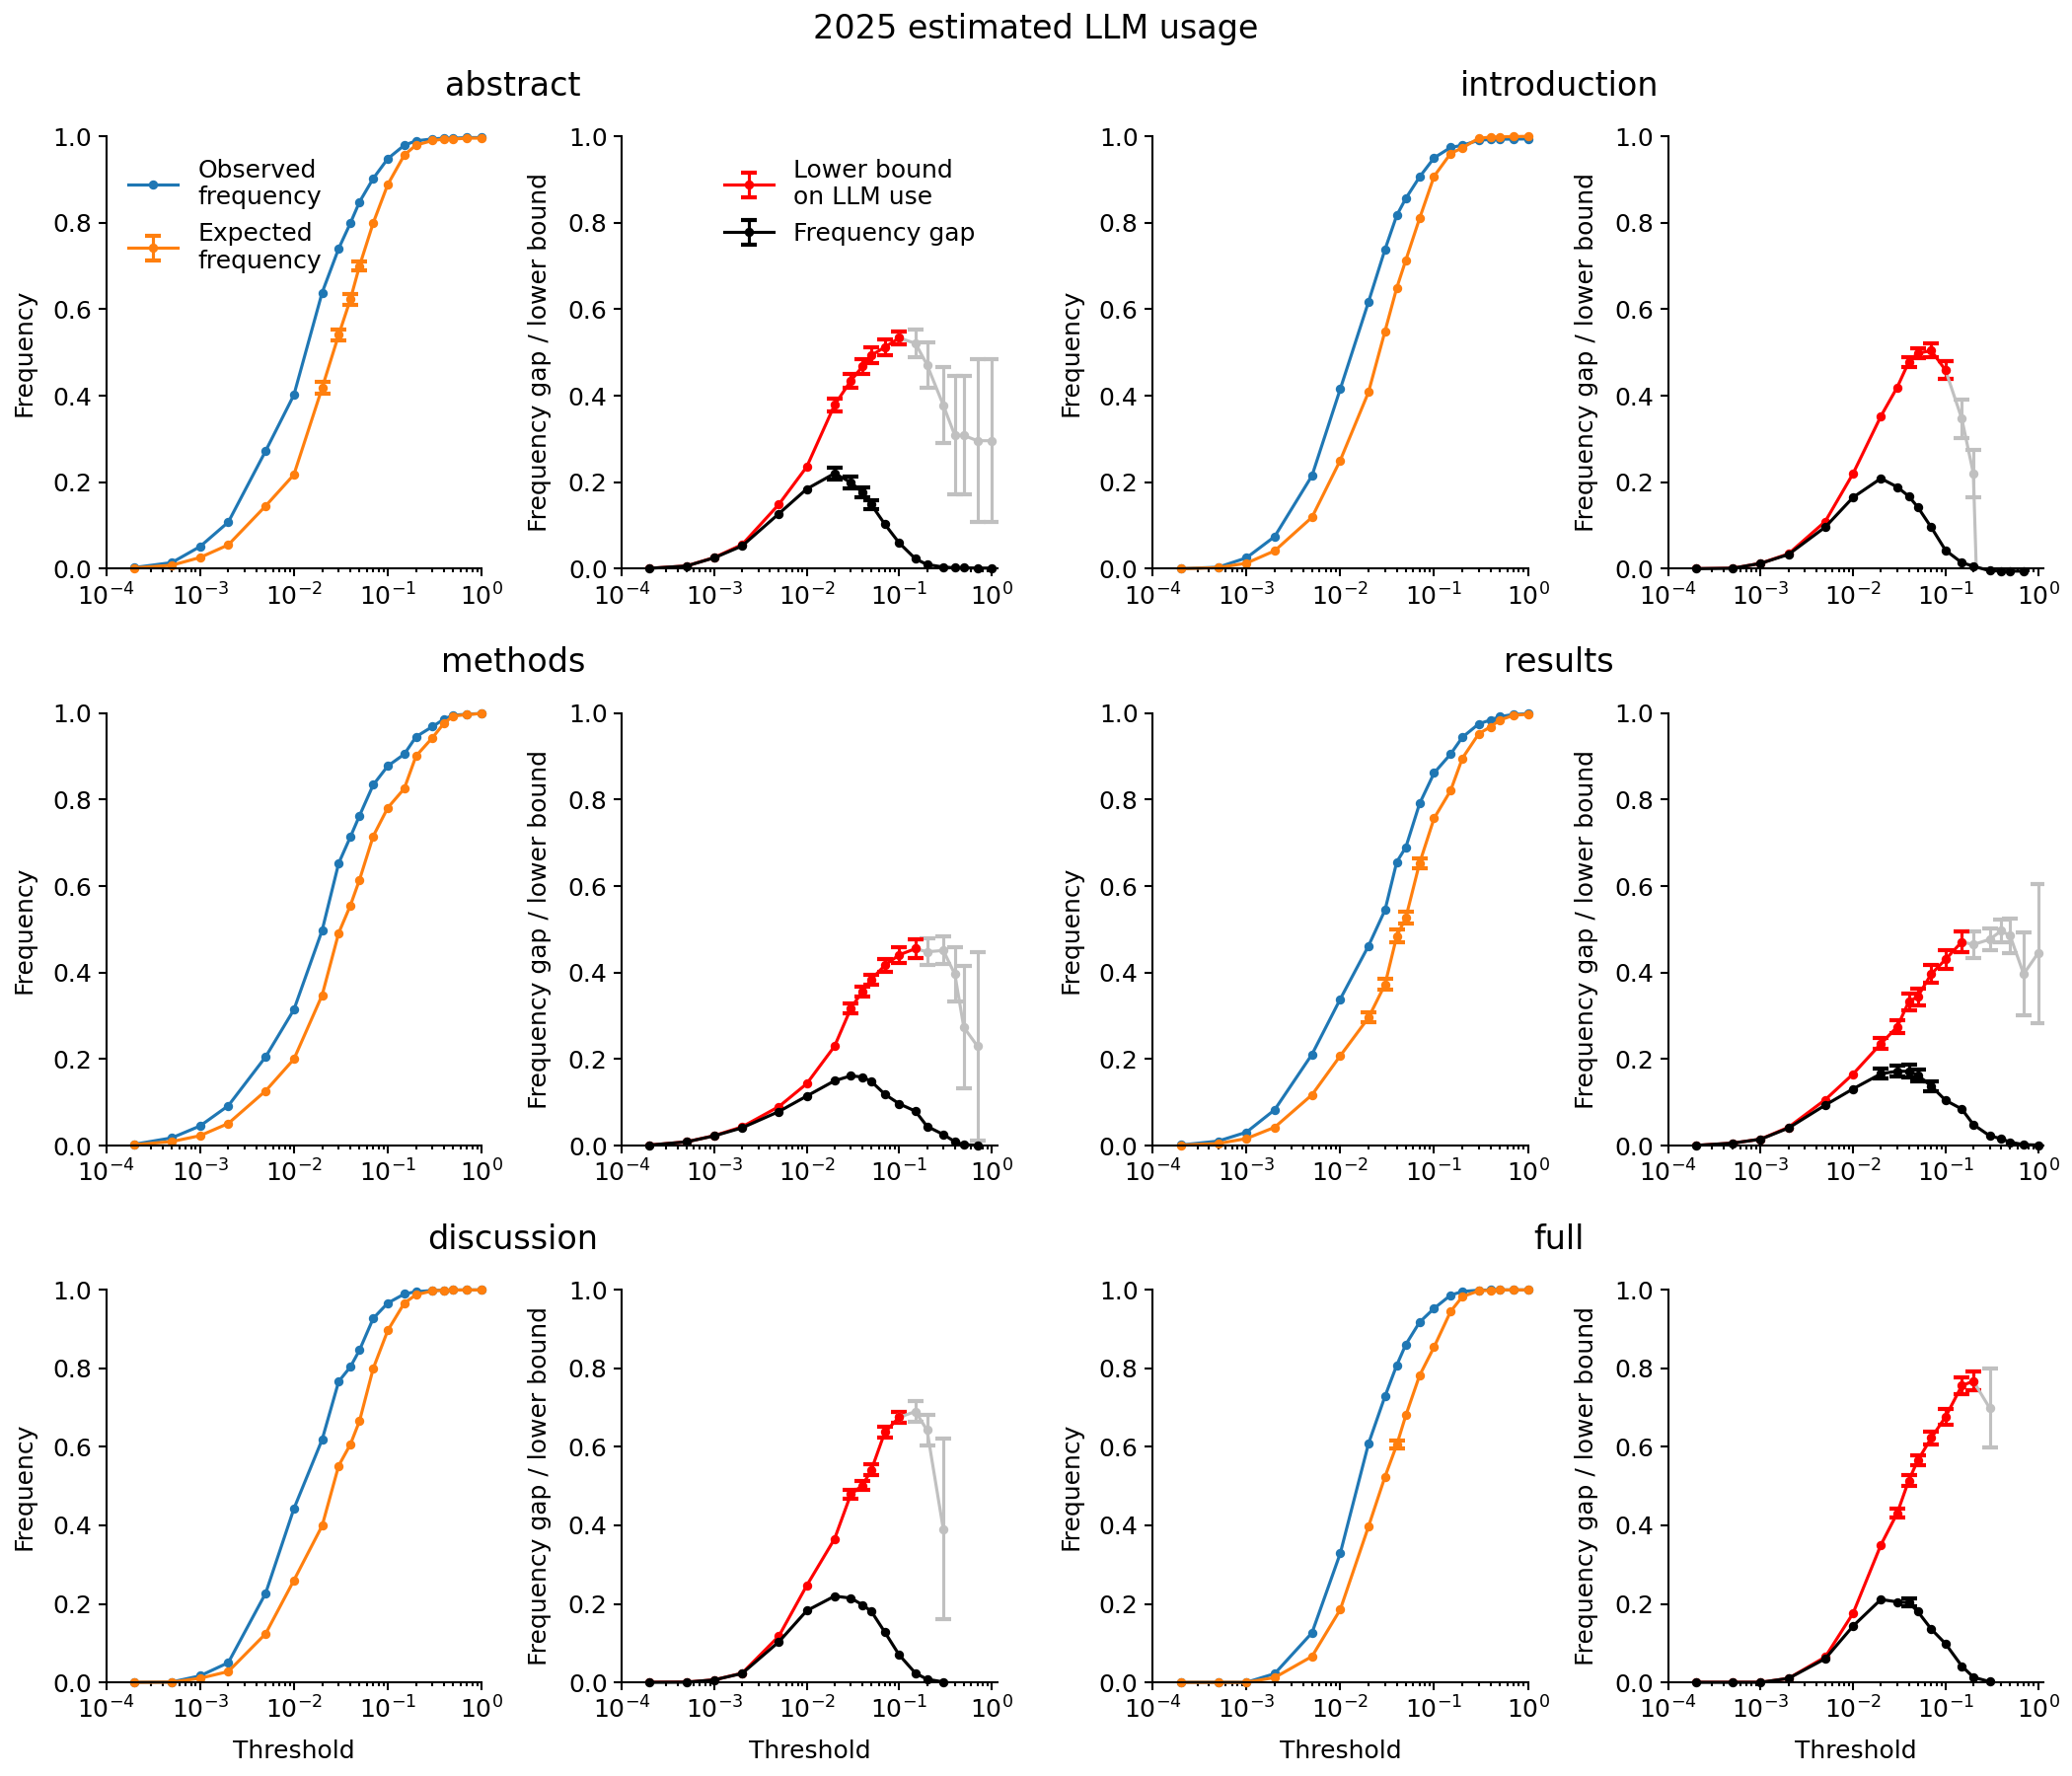
\includegraphics[width=\linewidth]{../results/plots/baseline_2026-01-23/research-article_aimrd_f/5y_2025_lower_bound_non_lemmatized_.png}
    \caption{}
    \label{fig:2025_optimization}
\end{figure}
\begin{figure}[htbp]
    \centering
    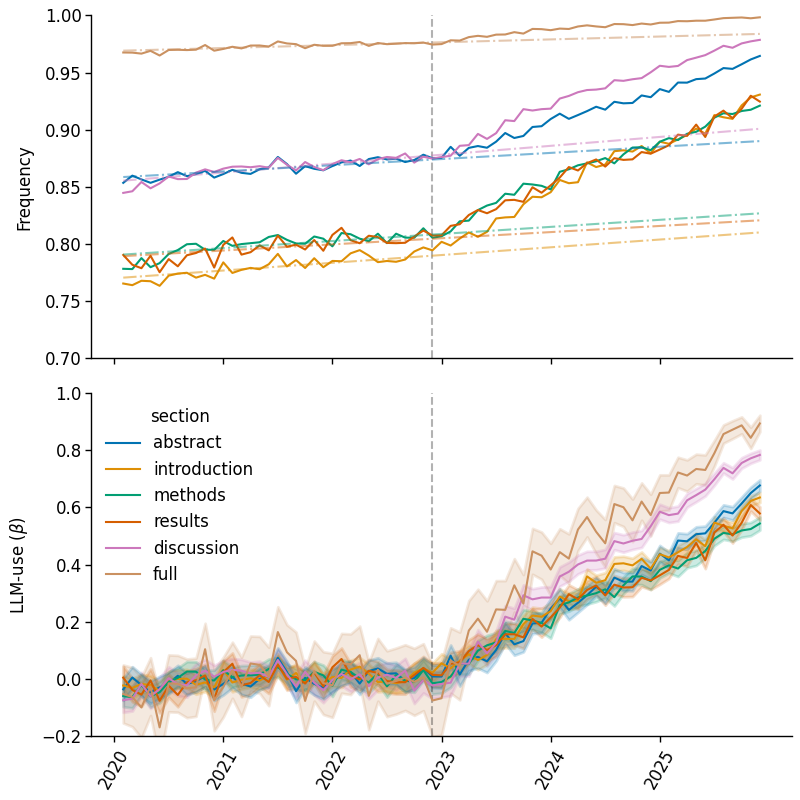
\includegraphics[width=\linewidth]{../results/plots/baseline_2026-01-23/research-article_aimrd_f/group_freqs_time.png}
    \caption{}
    \label{fig:monthly_est}
\end{figure}
\begin{figure}[htbp]
    \centering
    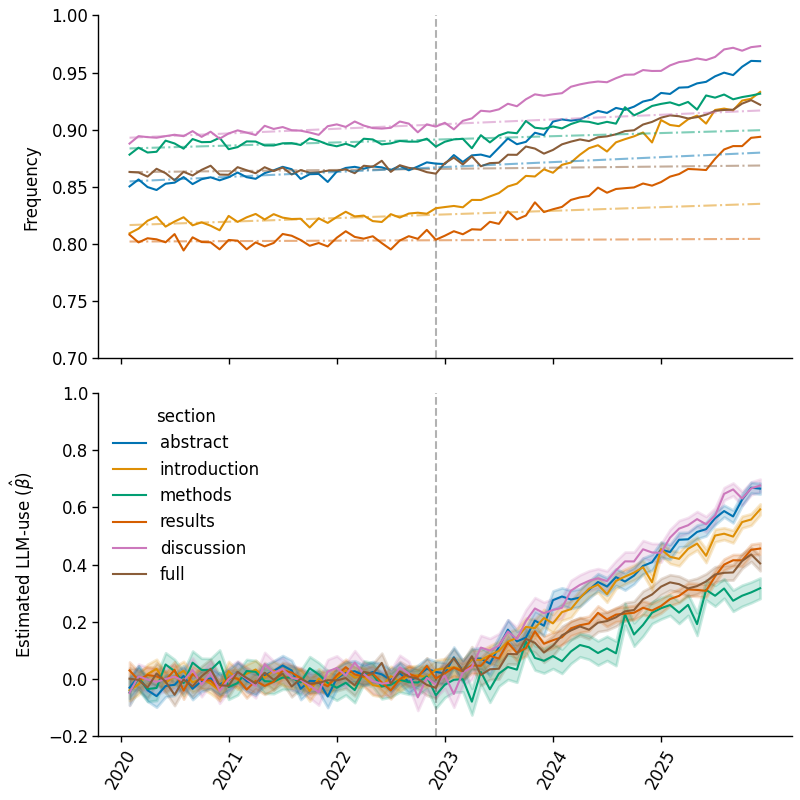
\includegraphics[width=\linewidth]{../results/plots/baseline_2026-01-23/research-article_aimrd_f_crop255/group_freqs_time.png}
    \caption{}
    \label{fig:monthly_est_crop255}
\end{figure}

\begin{figure}[htbp]
    \centering
    \begin{minipage}[t]{0.48\textwidth}
        \centering
        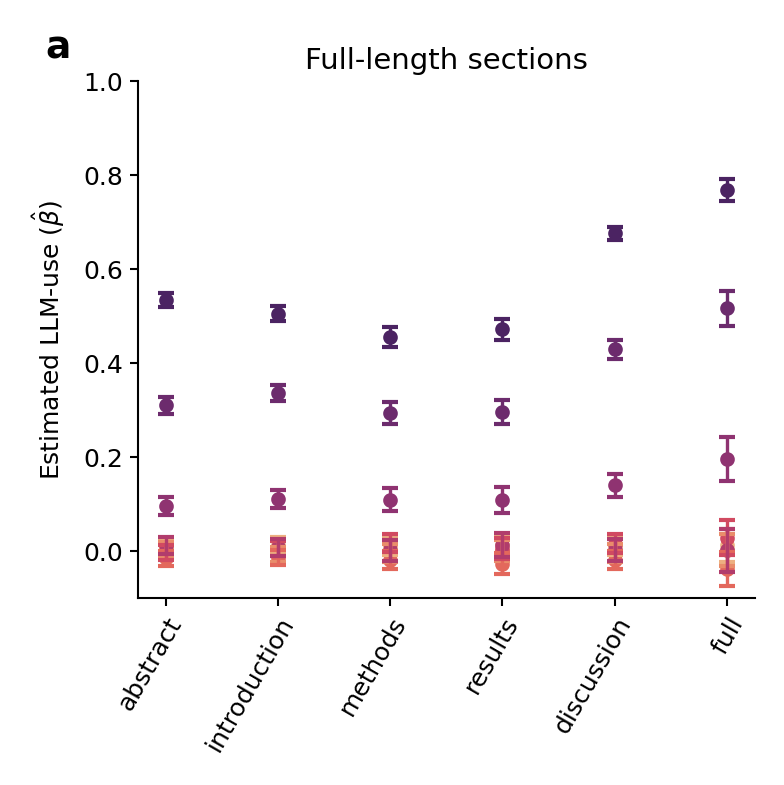
\includegraphics[width=\linewidth]{../results/plots/baseline_2026-01-23/research-article_aimrd_f/group_freqs_section_single_panel.png}
    \end{minipage}
    \hfill
    \begin{minipage}[t]{0.48\textwidth}
        \centering
        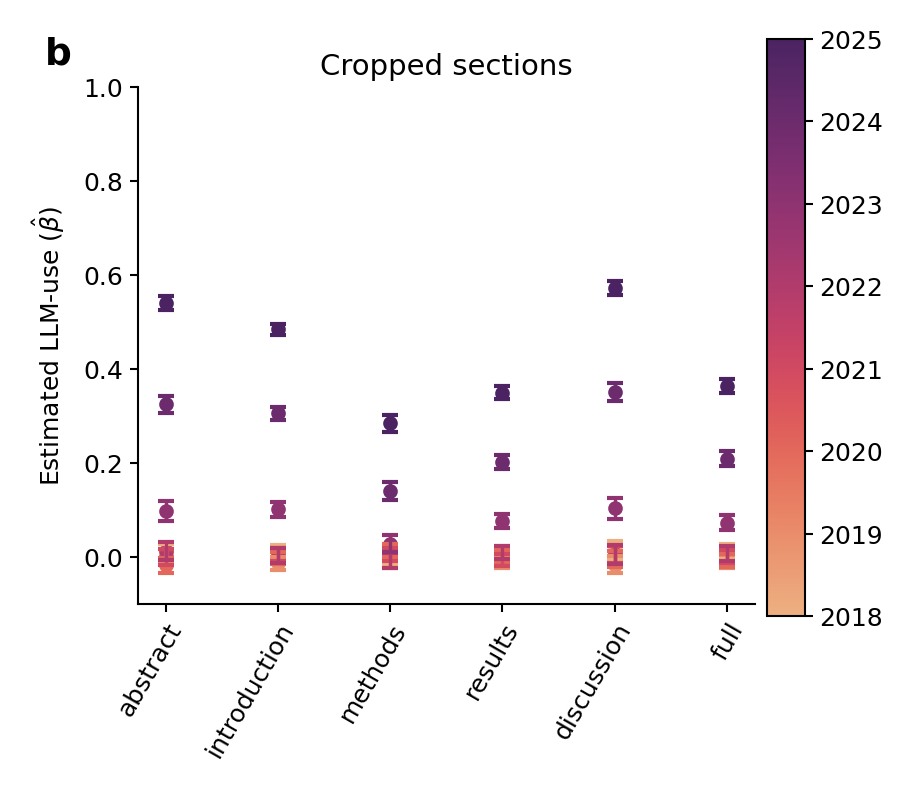
\includegraphics[width=\linewidth]{../results/plots/baseline_2026-01-23/research-article_aimrd_f_crop255/group_freqs_section_single_panel.png}
    \end{minipage}
    \caption{Shared caption describing both images}
    %comment: re-do this to only have one colorbar and title referring to full sections/cropped sections, also there should be no line connecting the dots 
    \label{fig:est_per_section}
\end{figure}
\section{Discussion}\label{sec:discussion}

\subsection{The estimate $\hbet$ reliably predicts LLM-use}
The LLM-use estimate $\hbet$ introduced in this work is a lower bound on actual LLM use derived from observed and counter-factual word frequencies. 
It makes use of the observation that LLMs show a preference for a group of words identified by Kobak et al., which they call excess style words  \cite{Kobak2025}.
By tracking the excess word frequency in a corpus before the wide-spread availability of Chatbots, we can estimate the frequency expected for the following years without the influence of LLMs on the writing process, $\hph$. 
To accurately determine LLM-use $\beta$, we would also need access to the frequency in a corpus of LLM-generated or LLM-assisted text.
Because this is not possible (without creating a curated collection of LLM-text), we replace $\pl$ with 1 in the equation for $\beta$, arriving at the lower bound $\hbet$.
\\
While $\hbet$ is a lower bound, it moves closer to true $\beta$ if $\pl$ gets closer to 1.
This can be achieved by selecting a group of words with collective high frequency to base the estimates on, which we do by incrementally increasing the frequency cutoff determining which words are selected for the word list, and computing the estimate for each list.
The danger of this approach is that if $\pl$ is very close to 1, so is $\hph$, resulting in both the numerator and denominator of the equation for $\hbet$ going towards 0, which causes strong fluctuation in the estimates, and yields division by zero errors in the worst case.
To avoid this, we constrain the search for the optimal cutoff such that $\hph$ must be below $0.999$ and the standard deviation error must be no bigger than $0.025$.
The simulation experiment tested the validity of this procedure.
We were able to identify the correct underlying proportion of LLM-assisted text for every ground-truth value tested.
This demonstrates the improvement toward the previous lower bound, $Delta$, which systematically underestimated LLM-use. 
Notably, some cutoff values that would have lead to an overestimation were excluded from the analysis by the constraints, indicating their importance.
The choice of $0.025$ as the maximum standard deviation is arbitrary, but has a potentially strong effect on the estimates.
For example, the estimate for LLM-use in the results section for 2025 would have been somewhat higher, if a higher threshold would have been chosen (see Figure \ref{fig:2025_optimization}).
Likewise, the estimates for the full paper reach their peak in the constrained regions for 2023 and 2024 (see Figures \ref{fig:2023_optimization} and \ref{fig:2023_optimization} in the Appendix).
On the other hand, as shown in Figure \ref{fig:simulation500} in the $30\%$ panel, overestimation of the true LLM-use is possible.
This should not happen in a lower bound metric, however, $\hbet$ is subject to some uncertainty, because it is computed with information that was empirically observed (in the case of $q$) or estimated with linear regression ($\hph$).
%comment: maybe depletion is predicted by q=1? but then all estimates would be 1, and this is not true for all depleted metrics. it can't be ph > q, cause then the estimate would be below 0, for the same reason it cant be ph>pllm, cause that implies ph > q, so what could it be?
The constraints on the standard deviation serve to keep this uncertainty in check, so the relatively conservative value of $0.025$ was chosen.
\\
Another peculiarity of the optimization curves is that they are almost always bell-shaped, and it is not clear why that should be the case.
Intuitively, the LLM-use estimates should increase with the number of words in the word list, as more words equal more LLM-markers to potentially be detected.
The bell shape could be an artifact of the estimates' increasing uncertainty.
To get a clearer image of this, we would need to adapt the frequency sampling for the simulations.
In the current version, the binomial probabilities that the simulation matrices are sampled from are distributed by a simple heuristic, such that the bulk of them have relatively low frequency with some outliers in the high-frequency region.
%comment: get a similar plot for distribution of real frequencies
However, in the optimization procedure, the observed and expected frequencies saturate to 1 much quicker than their empirical counterparts, such that they reach the constrained region of $\hph > 0.999$ earlier.
A sampling procedure yielding a distribution nearer to the empirically observed ones could improve understanding of the metric when both $q$ and $\hph$ are moving towards 1.

\subsection{LLM-use is continually on the rise across sections, countries and academic disciplines}
We observe a steady increase in LLM-use over the last three years, going up to $77\%$ in the main body of papers from 2025, and $89\%$ in the main body of papers from December 2025, the last time span considered here.
Using LLMs to edit or write certain parts of a paper has become commonplace in academia.
As shown in Figure \ref{fig:monthly_est}, this trend starts almost immediately after the release of ChatGPT, indicating a fast adoption of the new technology by scientists.
The rate of adoption also seems to follow a linear trend, which suggests that LLM-use is likely to continue growing in the future.
The pattern of continually increasing LLM-use also holds for the investigated subsets of PMC.
In all of the selected countries, language regions and academic disciplines, the highest LLM-use is observed in 2025, although the adoption is not as linear as in the combined set.
For example, the USA, the Netherlands and Brazil only show significant signs of LLM-use starting in 2024 (see Figure \ref{fig:countries_all}).

\subsection{LLMs are used more by NNES}
In line with our expectations, LLMs are used nearly twice as much in majority NNES countries as opposed to NES countries.
This trend has been reported in many other studies and surveys \cite{}. %comment: get citations.
An interesting country in this context is Canada, where people are NES only in some regions.
Accordingly, its LLM-usage is grouped between the NES and NNES countries.
The only outlier with regard to LLM-use is France, which has the third-to-lowest usage estimate in 2025 and the second-to-lowest in 2024 out of all investigated countries.
%how to explain? french people don't like technology?
Interestingly, the increasing use of LLMs seems to lead to the assimilation of the word frequencies in NNES and NES text. 
The frequencies of the selected word list was significantly higher in NES countries before the introduction of ChatGPT, but as of 2025, this gap is closed.
Because the word list only contains style words, this means that LLMs don't only help to avoid mistakes, but help users to adapt to a NES writing style, acting as ``linguistic equalizer'' \cite{Lin2025_NES,Prakash2025}.

\subsection{LLM-use estimates vary between (some) sections}
%comment: where to put this?: uncertainty and fluctuation is much bigger for full section, also exceeding the constraints, because the estimated were computed with the optimal word list for 2025, which might not be optimal for the previous years
%comment: need section length plot!

The LLM-use estimates of different sections were more similar than expected, with at most seven percentage-points differentiating the abstract, introduction, methods and results, with the abstract yielding the highest estimate among the four in 2025, but being second to the introduction in 2024.
The discussion is clearly the section with highest LLM-use, with estimates up to fifteen percentage-points higher than the abstract.
Because the estimates for the main body of the paper includes all sections except the abstract, and there are individual sections with higher estimated LLM-use than the abstract, the main body estimates are necessarily the highest, because they are an upper bound for the other sections.
This is because we calculate word occurrence and not word frequency within a text as the basis for our frequency measure, so if a word appears in any one section, it also appears in the full text.
\\
The big gap between estimates for individual sections to those of the full paper indicate that it's not the case that LLMs are always used uniformly across the paper, such that a high LLM-use estimate in one section doesn't necessarily predict high LLM-use in other sections.
Instead, many papers seem to have been written with relatively selective use of LLMs, where only certain sections were altered.
On the other hand, the LLM-use estimates of the discussion are not much smaller than those of the full paper, indicating that if there were LLM-generated passages somewhere in a paper, it would most likely be in the discussion.
Also, even with the gap between full paper estimate and individual sections estimates present, it is not nearly big enough to indicate that only one section per paper had been edited (this also would be a highly unlikely scenario).
All in all, this suggests the most common use of LLMs is to edit certain paragraphs of the paper, that might or might not be in the same section, with the discussion having the highest likelihood of being edited.
To further investigate this, sections could be grouped in the counting process, to indicate whether a marker word occurs in both sections.
\\
These observations alleviate a potential concern of our method, namely that the excess words identified in 2024 PubMed abstracts would be vocabulary tailored specifically to abstracts, and thus would only reliably pick up on LLM-use within abstracts.
To guard against this, the excess word list was sorted according to the frequencies within each section during optimization, and each section was optimized separately (although, as previously discussed, the individual optimization means that some sections might be impacted more by the constraints than others).
It could still be that LLM-use in all sections except the abstract is underestimated, but as the discussion and, for some intervals, the introduction yield higher estimates than the abstract, it is at least not the case that our method favors the abstract to the point of always attributing highest LLM-use to it.
In fact, when looking at the results for different countries and disciplines, the main body of the text almost always yields higher estimates than the abstract, the only exceptions being Australia and France, which, as discussed previously, is an outlier in other regards as well.
\\
Of course, the abstract is by far the shortest of the investigated sections, and is much shorter when compared to the main body of the text.
There are many more paragraphs that could have been rewritten with the help of an LLM, many more words that could have been replaced with marker words while editing.
To normalize for section length and investigate how likely it is for any paragraph within a section to have been altered with the help of LLMs, we repeated the experiments with cropped versions of the sections.
%comment: it's not really normalization
There is barely any difference between the LLM-use estimates of the full and cropped abstracts, which is to be expected as any random crop of 255 words (the median length of the abstracts) will contain most or all of the abstract in question.
The difference between full and cropped introductions is also very small (two percentage points, which is within one of the error margins), indicating that if an LLM was used to edit the introduction, changes were made to the entire section as opposed to single paragraphs.
For results and discussion, the changes from full to cropped are somewhat larger, with twelve and eleven percentage points respectively.
This indicates that while LLM-use is still relatively evenly spread among different paragraphs in these sections, there appears to be some clustering of markers.
The biggest difference between the full and cropped versions is measured in the methods section, showing that LLM-use is most clustered here.
However, it could also be that there are more linguistic restrictions in certain parts of the methods section, which don't allow the replacement of words with LLM markers. 
For example, reporting the technical details of some experimental setup usually follows a typical structure that doesn't leave space for the style words we use to detect LLM-use.
This means that LLMs might be used universally in all paragraphs of the methods section, but only change the vocabulary in some.
\\
Overall, a single paragraph sampled from the discussion or abstract has the highest likelihood of having been edited with an LLM, followed by the introduction, results and full text, with methods coming last.

\subsection{Comparison to other estimation methods}
 - advantage of not relying on ground-truth text: not vulnerable to different results stemming from different prompting strategies (Dou enhancing robustness 2024) (disadvantage is only lower bound, but as was shown, we get reasonably close to the actual value)
- going beyond word frequency: other linguistic markers as LLM indicators (perplexity, sentiment, part-of-speech, vocab size and density) e.g. \cite{Guo2023}, Bao Tong 2025, or intrinsic text embedding dimensionality \cite{Tulchinskii2023}, or repeated higher-order n-grams \cite{Gall2021} (although this is for GPT2 and might be no longer true)


\subsection{Limitations}
Some concerns about our method have already been discussed in previous sections of the discussion.
The LLM-use estimate $\hbet$ behaves unreliably in the limit regions where $q$ and $\hph$ go towards one, which is critical because this is also the area in which it is most likely that $\pl=1$, thus giving the most reliable results.
The constraints introduced to avoid unreliable estimates in the limits may lead to a disparity between sections, as the sections are optimized individually, so for some, the optimal estimate might lie in the constrained region. 
Because suboptimal estimates are to be preferred to unreliable ones, the constraints were kept at a relatively conservative level. 
Another limitation is our inability to perform excess word search for each section in our dataset, being limited to using the list established in prior research by Kobak et al. \cite{Kobak2025}.
Since the excess words are domain-independent, %comment: are they?
they should have equal validity for each section and the optimization procedure is still section-specific.
\\
A more severe limitation is that our estimates are, by design, dependent on changes in word frequency between human and LLM-generated text.
By using only marker words, we are unable to detect LLM-generated text that, by using a distinct prompting strategy \cite{Geng2025} or by chance, doesn't contain any excess words.
This is somewhat mitigated by the length of the excess word list, it is much harder to purposefully or accidentally exclude over 300 words, compared to the small selection used by other authors \cite{Gray2025, Gray2026, Kousha2025}.
However, the main concern doesn't focus on $\pl$, but on $\ph$.
Our estimate hinges on the central assumption that $\hph$ is a faithful estimate of $\ph$. 
For the months immediately following the release of ChatGPT, this is a reasonable assumption, as $\ph$ follows a linear trend that can be modelled with linear regression.
As we move away from this date, confidence in $\hph$ decreases, because the environment that academic text is produced in fundamentally changes with the introduction of LLMs.
The more papers are written with the help of LLMs, the more people will become familiar with their writing style, and might start consciously or subconsciously copying it.
They might also use LLMs for other tasks, thereby learning the types of suggestions LLMs typically make and adapting those into their own writing process, without repeated input from the LLM.
LLMs have already been shown to influence human speech.
Yakura et al. \cite{Yakura2025} investigated changes in word frequency in academic talks on YouTube and conversational podcast episodes and found increasing use of ``delve'' after November 2022 in both datasets.
While both of these media forms rely on scripted content to some extent (the podcasts showing hints of LLM-use were educational and situated in the realms of science and technology, business and education, rather than casual conversations), the podcasts will likely also contain segments of spontaneous speech. 
Even though there is some evidence for the influence of LLMs on human speech, it is unclear how quick and how pervasive this adaption to an LLM-style of writing will take place.
Previously uncommon words like ``delve'' are very salient signals because their sudden appearance after relative obscurity generates more attention \cite{Geng2025}.
This also makes them more likely to be copied, especially for NNES who might not have known the word previously and added it to their vocabulary only after coming across it in LLM-generated text.
On the other hand, changes in the frequency of common words are much harder to pick up on.
When reading a text, it doesn't really make a difference to the reader if the word ``these'' appears two or three times.
Changes in high-frequency words only really register when looking at a large corpus of text, whereas humans interacting with LLMs or reading LLM-assisted papers only have access to a small selection.
This makes it less likely for them to be copied directly.
Geng and Trotta \cite{Geng2025} therefore argue for focussing on high-frequency words when trying to detect LLM-generated text, although with the rising influence of LLMs, it is unclear for how long this advantage will hold.
High-frequency words might for example be part of certain phrases that LLMs prefer, which could be copied by users.
To investigate this, the analysis could be widened to include higher-order n-grams.


\subsection{Impact}
impact / normative evaluation: overcoming language barriers, science papers rely on the data that is being reported, writing style is not immediately important. However, writing is a technology to sharpen our thinking. It takes effort to write something down. In deciding how exactly to phrase something, we are forced to think very precisely about our work, a level of scrutiny which makes it more likely that leaps of logic will be addressed that would have been brushed by when only engaging with LLM outputs



\printbibliography

\appendix
\section{Survey results}
In all surveys, we focused on use cases that could have an influence on the formulation if final paper, such as editing or summarizing of other papers, instead of use cases in other academic undertakings, such as writing code, or very early in the writing process, like brainstorming or writing an outline.
Grammar checks were also excluded as a relevant use case, because while this is a very popular task for LLMs, this should have a minor influence on phrasing.
If use cases were not part of the survey, we took the general proportion of researchers reporting LLM use in at least some part of their research. 
an important factor in evaluating the results is the organization doing the survey.
Researchers might be hesitant to admit LLM use in a survey done by an important academic publisher despite anonymity, especially if this publisher is known to be anti-LLM, such as Nature

\begin{sidewaystable}
\centering
\begin{tabular}{lrlllrc}
\toprule
\makecell[c]{survey\\period} & \makecell[c]{sample\\size} & \makecell[c]{sample\\specification} & \makecell[c]{question} & \makecell[c]{category} & \makecell[c]{usage} & \makecell[c]{source}\\
\midrule

\multirow{2}{*}{\makecell[l]{04/2023--\\05/2023}}
& \multirow{2}{*}{456} 
& \multirow{2}{*}{urologists} 
& Do you use ChatGPT/LLMs in your academic practice? 
& general & 48\% 
& \multirow{2}{*}{\cite{Eppler2024}}\\
&&& summarizing text & writing & 27\% &\\

\midrule

\multirow{2}{*}{\makecell[l]{06/2023--\\07/2023}} 
& \multirow{2}{*}{3,838} 
& \multirow{2}{*}{postdocs} 
& Do you use AI chatbots, such as ChatGPT, in your work? 
& general & 31\% 
& \multirow{2}{*}{\cite{Nordling2023}}\\
&&& \makecell[l]{What do you use AI chatbots for? Refining text} 
& editing & 20\% &\\

\midrule

\makecell[l]{?--\\09/2023} 
& 1,659 
& \makecell[l]{researchers who\\had published\\in Q4 2022} 
& \makecell[l]{What do you use generative AI tools (e.g., ChatGPT, \\LLMs) for? To help write research manuscripts} 
& writing & 21\% 
& \cite{VanNoorden2023}\\

\midrule

\multirow{5}{*}{\makecell[l]{11/2023--\\04/2024}} 
& \multirow{5}{*}{816} 
& \multirow{5}{*}{\makecell[l]{researchers\\(Semantic\\Scholar)}} 
& Fix grammar or rephrase 
& editing & 50\% 
& \multirow{5}{*}{\cite{Liao2024}}\\
&&& Rewrite for another style & writing & 24\% &\\
&&& Shorten or summarize & writing & 23\% &\\
&&& Draft paragraphs from ideas & writing & 21\% &\\
&&& Direct writing (overall) & writing & 43\% &\\

\midrule

\makecell[l]{12/2023--\\02/2024} 
& 2,284 
& \makecell[l]{clinicians \&\\researchers} 
& \makecell[l]{Have you used an AI product or AI feature\\for a specific work-related purpose?} 
& general & 37\% 
& \cite{Elsevier2024}\\

\midrule

\multirow{3}{*}{\makecell[l]{01/2024--\\03/2024}}
& \multirow{3}{*}{2,021} 
& \multirow{3}{*}{\makecell[l]{researchers\\(Scopus)}} 
& \makecell[l]{Why use ChatGPT/AI tools:\\Synthesizing drafts to academic text} 
& \makecell[l]{\\writing} 
& \makecell[r]{\\16\%} 
& \multirow{3}{*}{\cite{Mohammadi2026}}\\
&&& Proofreading drafts & editing & 17\% &\\
&&& Translating text & writing & 18\% &\\

\midrule

\multirow{2}{*}{\makecell[l]{03/2024--\\04/2024}} 
& \multirow{2}{*}{1,043} 
& \multirow{2}{*}{researchers} 
& Help with translation & writing
& 40\% 
& \multirow{2}{*}{\cite{Wiley2025}}\\
&&& proofreading and editing scholarly papers & editing & 38\% &\\

\midrule

\multirow{4}{*}{\makecell[l]{03/2024--\\05/2024}} 
& \multirow{4}{*}{5,229} 
& \multirow{4}{*}{researchers} 
& Have you used AI to edit your paper? & editing
& 28\% 
& \multirow{4}{*}{\cite{Kwon2025}}\\
&&& ... to translate your paper? & writing & 8\% &\\
&&& \makecell[l]{... to summarize other papers for use in your own?} 
& writing & 8\% &\\
&&& ... to write the first draft of your paper? & writing & 8\% &\\

\midrule

\multirow{2}{*}{\makecell[l]{04/2024--\\06/2024}} 
& \multirow{2}{*}{226} 
& \multirow{2}{*}{\makecell[l]{medical\\researchers}} 
& Stage of publication LLM used: Writing 
& writing & 8\% 
& \multirow{2}{*}{\cite{Mishra2024}}\\
&&& Revision and editing & editing & 8\% &\\

\bottomrule
\end{tabular}
\caption{Summary of survey results on AI/LLM usage in academic and clinical research}
\label{tab:placeholder}
\end{sidewaystable}
\section{2024 excess words}\label{ap:wordlist}

The following is a list of all excess style words identified by \cite{Kobak2025}.
They are sorted from least to most frequent, as measured for abstracts in PMC.
\\\\
\emph{revolves, upholding, dependability, attains, endeavours, scrutinizing, garnering, consolidates, encapsulates, merges, accentuates, grappling, acknowledges, furnish, delving, solidify, uphold, urging, surmount, juxtaposed, customizing, propelling, detrimentally, interconnectedness, equipping, realms, categorizes, commendable, embracing, crafting, substantiates, bolstered, pioneers, burgeoning, unlocking, capitalizing, heighten, gauged, emulating, refines, uncharted, unparalleled, crafted‘, adept, scrutinize, swiftly, emulation, excels, surged, harnesses, revolutionizing, spurred, streamlines, expediting, dependable, bolstering, empowers, groundbreaking, illuminating, hinting, discerning, afflicted, inquiries, scrutinized, detailing, discerned, surpass, overlook, streamlining, emphasising, delineates, seamless, overlooking, seamlessly, hinges, emphasises, acknowledging, revolutionize, fosters, pinpointing, nuances, swift, advocating, meticulous, strategically, signifying, delved, illuminates, surpasses, amidst, renowned, outlines, complicating, spanned, showcased, intricacies, advocates, adhering, bolster, categorizing, poised, stemming, delve, expedite, formidable, affirming, complicates, pioneering, endeavors, culminating, elevates, delves, adhered, intricately, comprehending, showcases, substantiated, streamline, transformative, unveiling, meticulously, streamlined, harness, realm, surpassed, enduring, pinpointed, distinctions, impressive, imbalances, inadequately, exceptionally, necessitate, discernible, elevating, elevate, exerting, invaluable, struggle, enhancements, showcasing, aligns, encompass, diminishing, unraveling, harnessing, discern, diminishes, akin, garnered, refining, impeding, escalating, exacerbating, augmenting, orchestrating, impede, warranting, pinpoint, foundational, groundwork, seeks, underscored, encompasses, pressing, combating, versatility, unveils, surpassing, aligning, posed, paving, fostering, featuring, noteworthy, elucidates, necessitates, stands, uncovering, aiding, posing, leverages, hinder, exceptional, encompassed, nuanced, compelling, refine, incorporates, underexplored, thorough, employs, align, recognizing, evaluates, methodologies, correlating, addresses, unveiled, utilizes, unveil, necessitating, multifaceted, imperative, exceeding, emerges, evolving, displaying, integrates, yielding, avenue, disrupts, introduces, examines, advancement, shedding, emphasizes, elucidating, preserving, persist, distinctive, inherent, necessity, serving, advancements, optimizing, advancing, explores, spanning, underscoring, shaping, avenues, hold, impacting, emphasize, ensuring, encompassing, pose, emphasizing, heightened, remarkable, unexplored, leveraging, intricate, investigates, broader, alongside, serves, holds, poses, capabilities, facilitated, facilitates, innovative, employing, initially, underscores, exploration, exhibiting, incorporating, attributed, interplay, pronounced, involves, addressing, comprising, revealing, notable, ultimately, integrating, categorized, underscore, facilitating, conversely, achieving, focusing, consequently, promise, exhibits, predominantly, influencing, enabling, presents, integration, offering, typically, demonstrating, varying, assessments, enhances, maintaining, pivotal, utilizing, contributing, precise, limitations, elucidate, emerged, offers, assessing, highlighting, offer, reveals, prevalent, involving, techniques, subsequently, primarily, enhancing, demonstrates, utilized, substantial, exhibit, challenge, thereby, valuable, challenges, effectively, highlights, address, highlight, employed, providing, enhance, specifically, indicating, diverse, notably, comprehensive, resulting, potentially, elevated, linked, promising, leading, aims, enhanced, distinct, particularly, despite, need, strategies, insights, crucial, exhibited, like, conditions, complex, additionally, individuals, various, assess, understanding, approach, remains, primary, assessed, impact, outcomes, demonstrated, conducted, across, research, within, revealed, observed, through, role, identified, while, including, into, potential, findings, both, their, using, these, this} 

\section{Additional simulation results}
\begin{figure}[htbp]
    \centering
    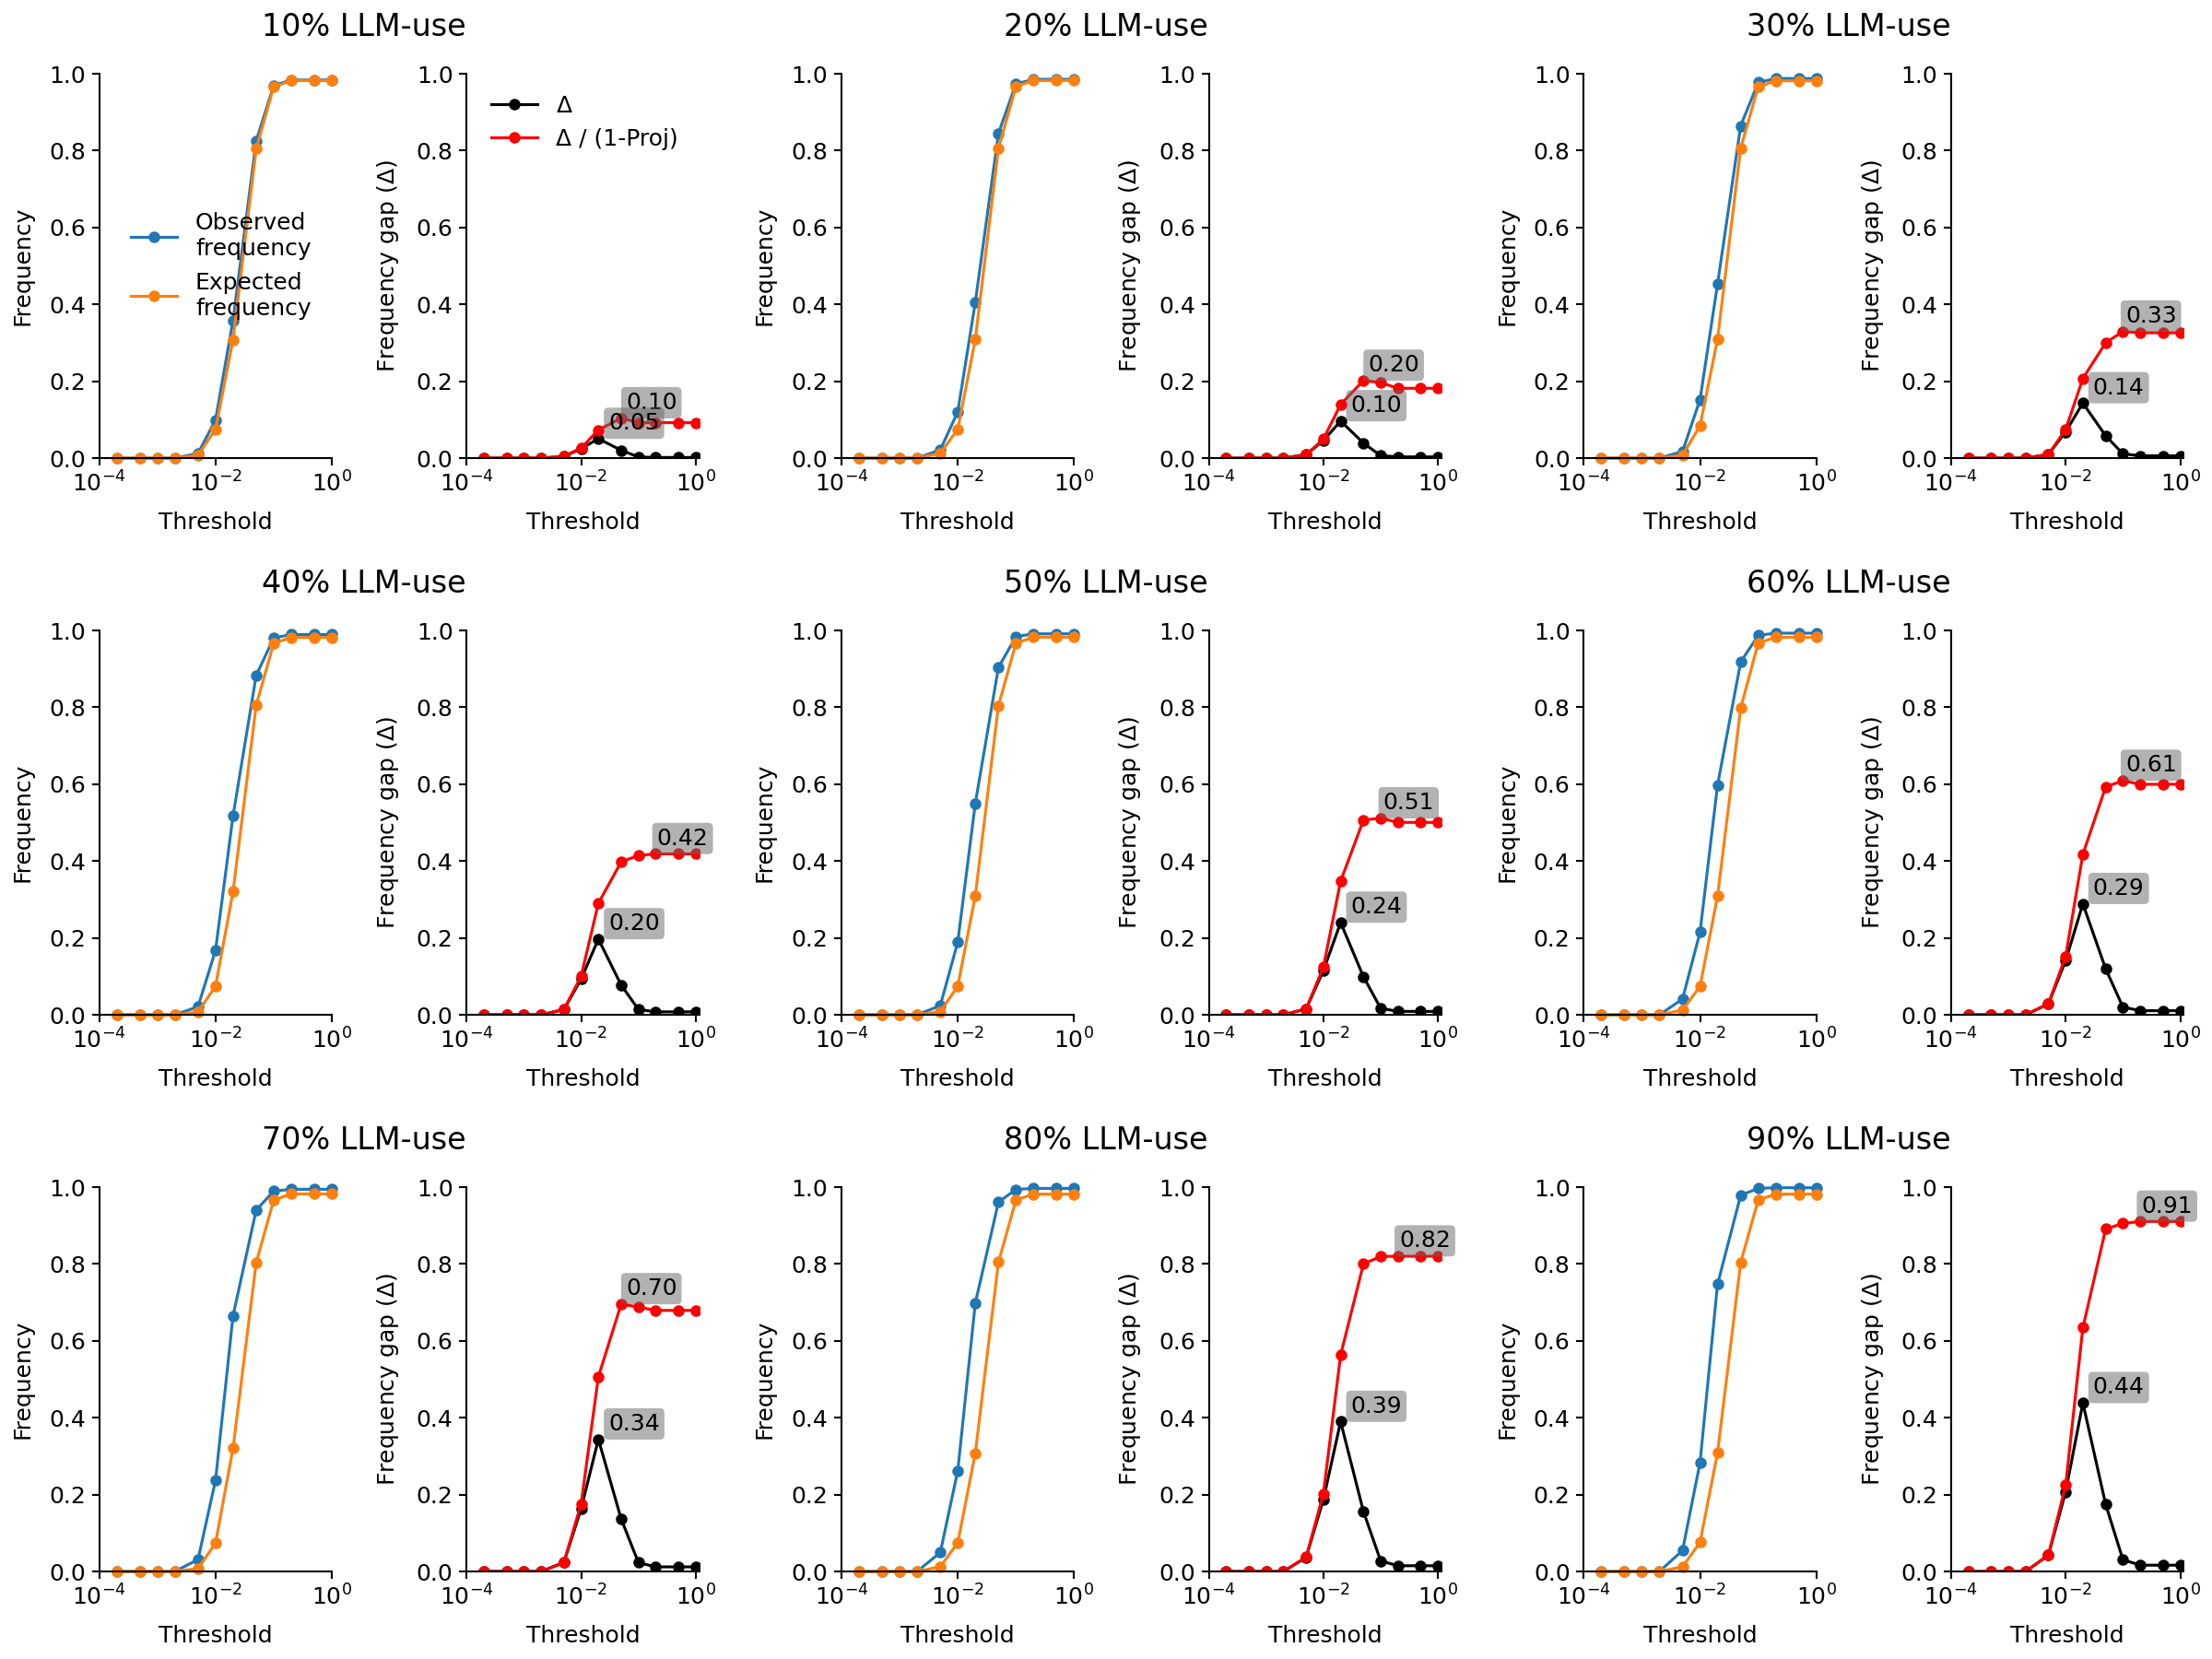
\includegraphics[width=\linewidth]{../results/plots/ground_truth_simulation/100_words.png}
    \caption{}
    \label{fig:simulation100}
\end{figure}
\begin{figure}[htbp]
    \centering
    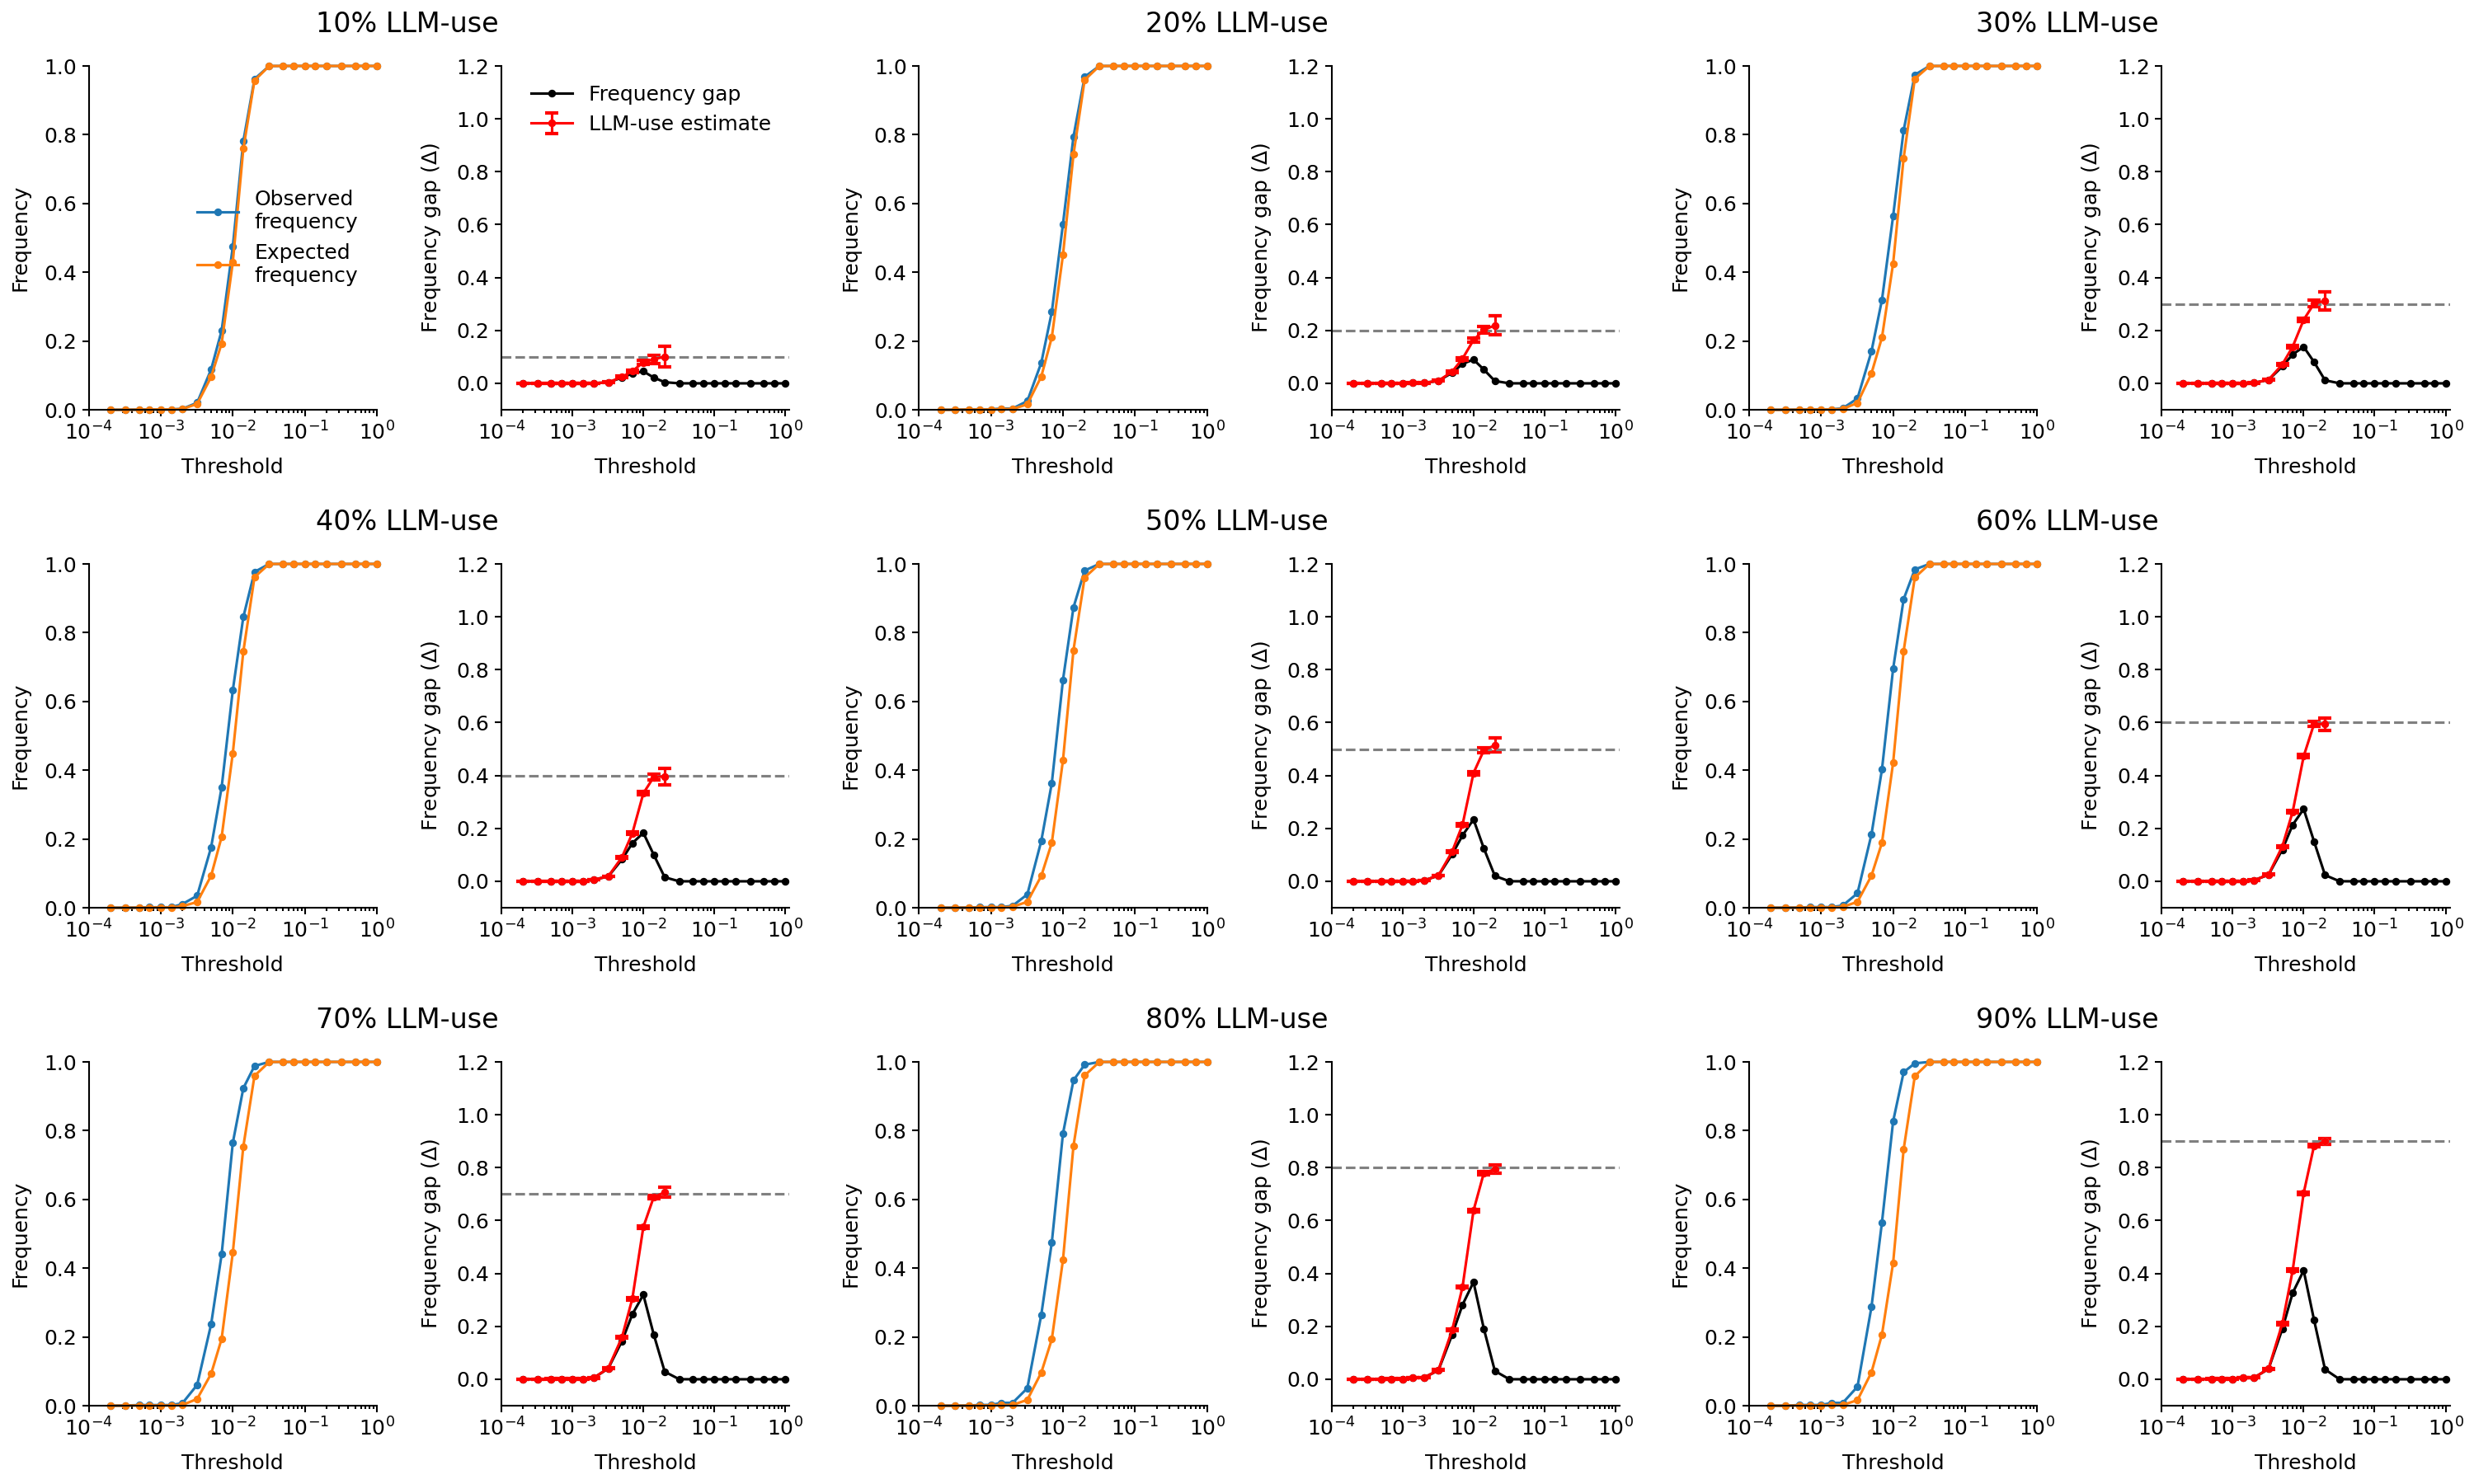
\includegraphics[width=\linewidth]{../results/plots/ground_truth_simulation/1000_words.png}
    \caption{}
    \label{fig:simulation1000}
\end{figure}
\section{Word list optimization}\label{ap:opt}
\begin{figure}[htbp]
    \centering
    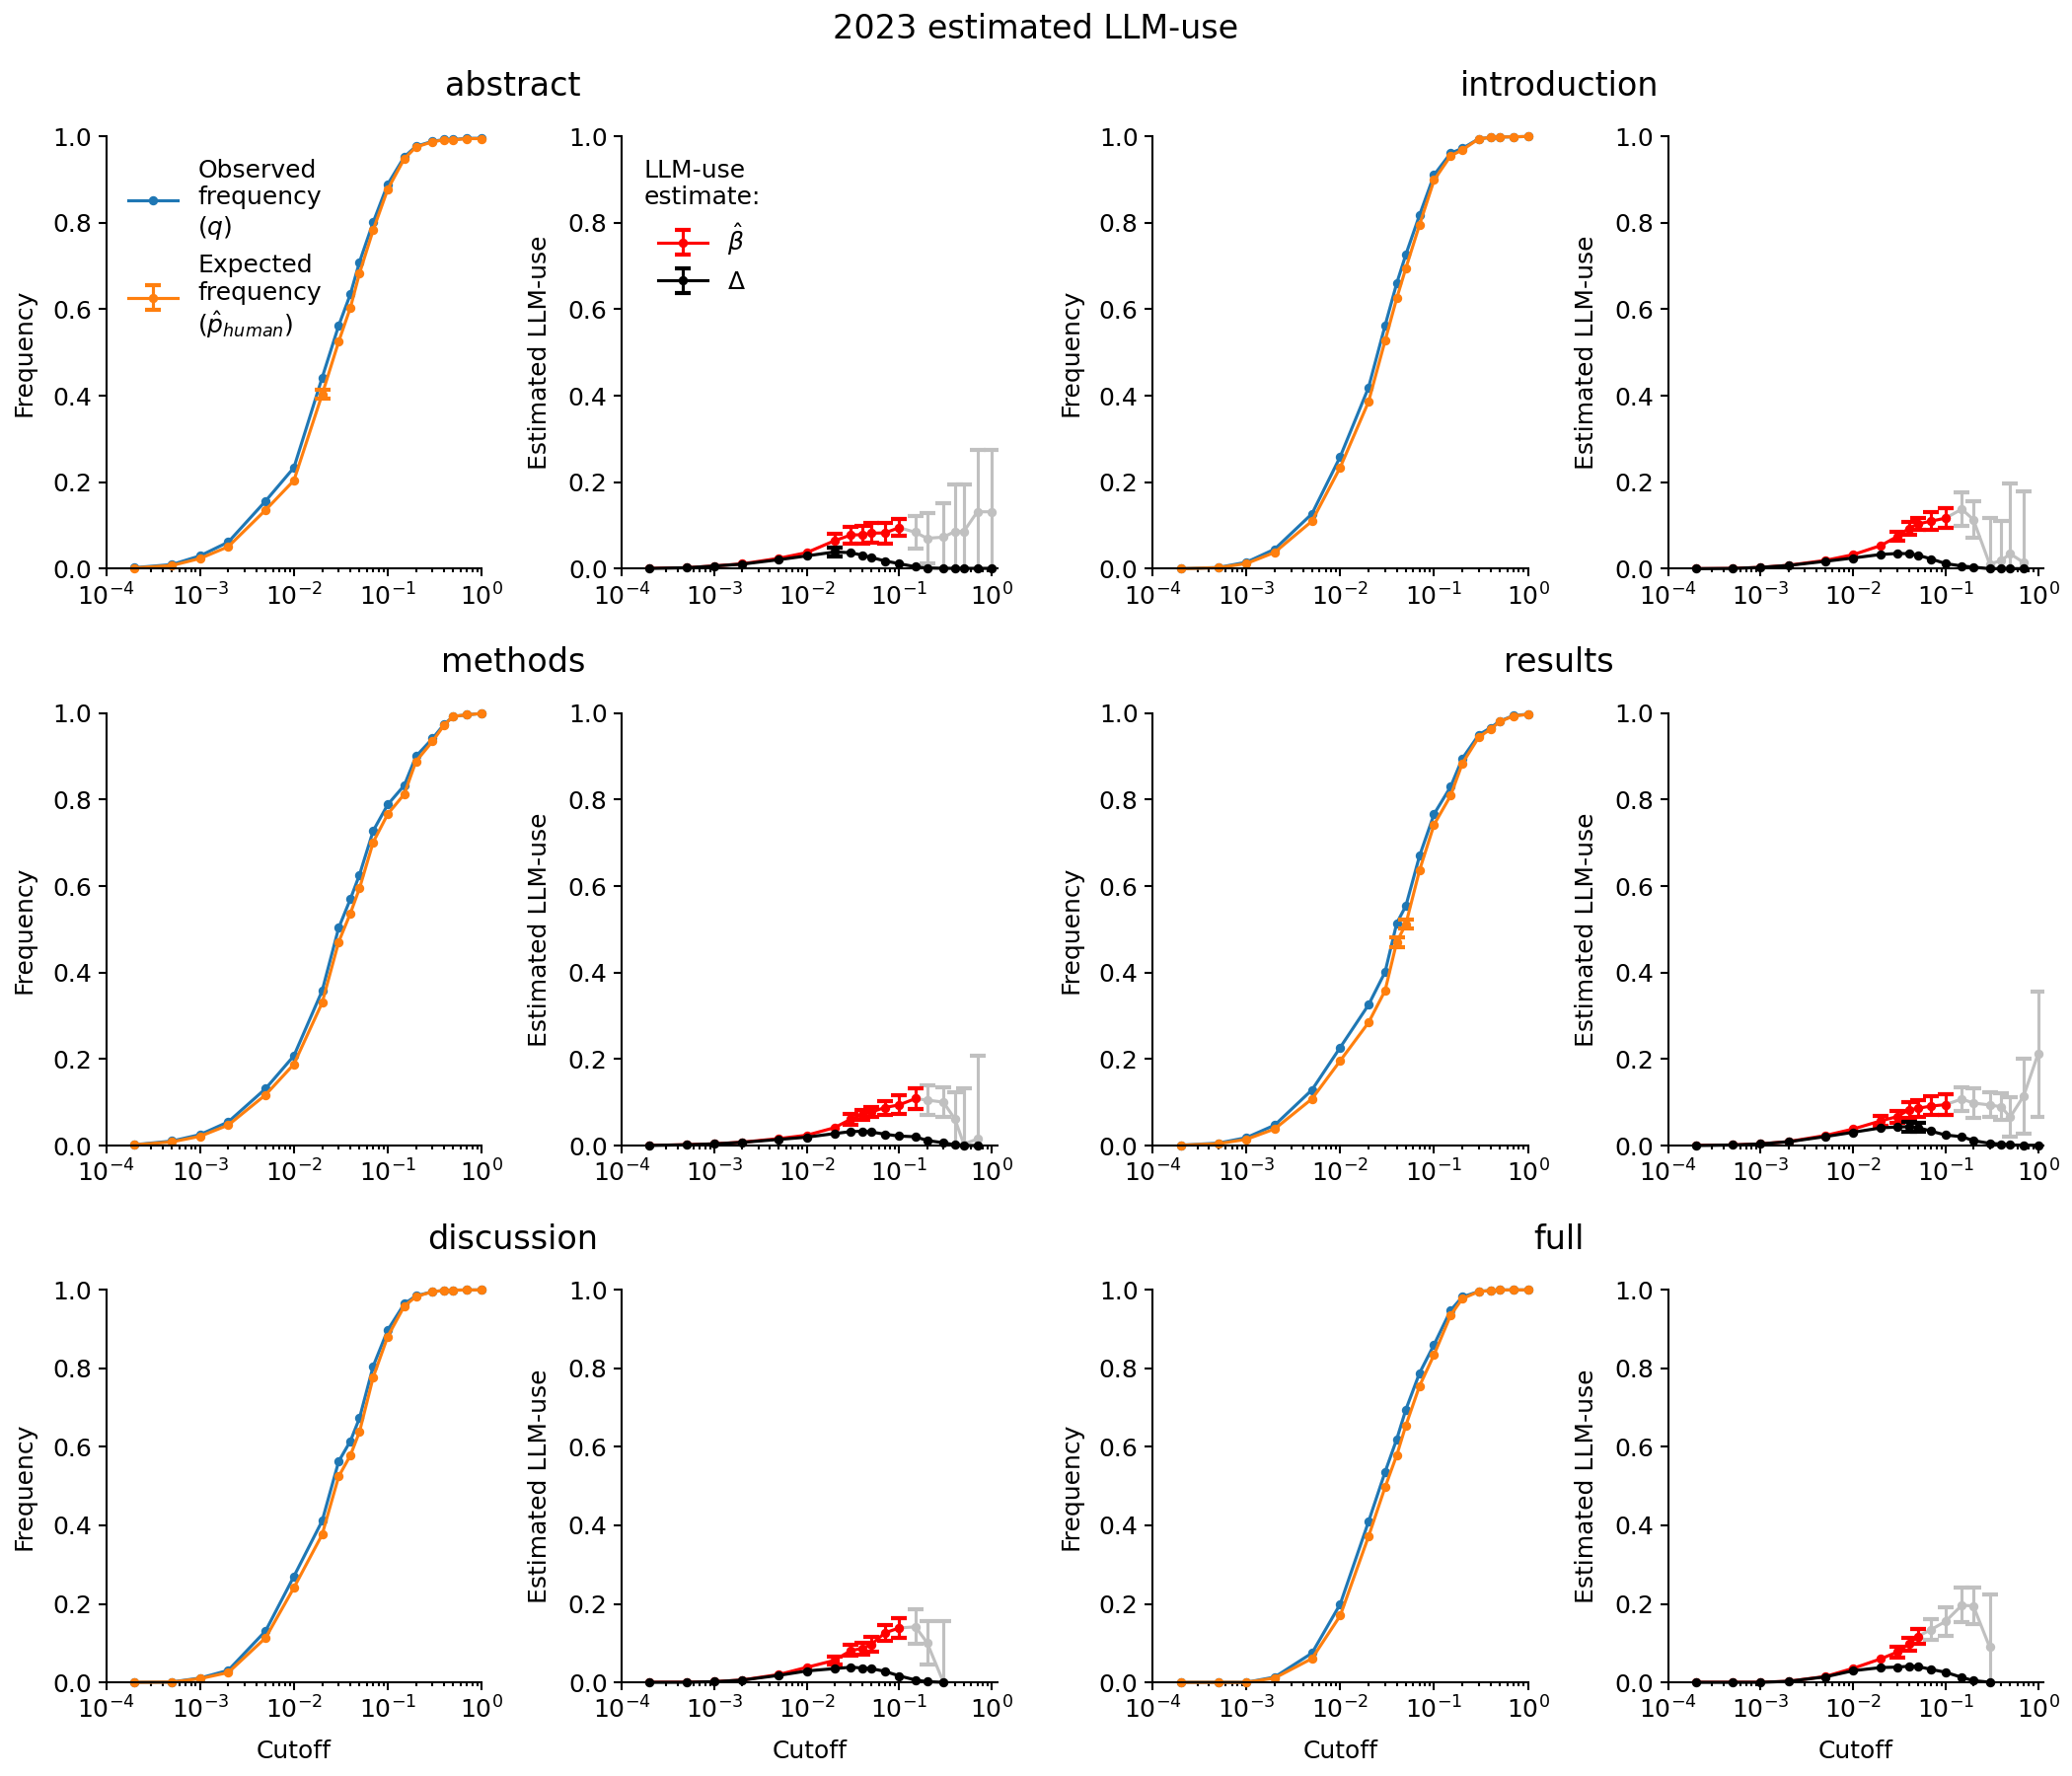
\includegraphics[width=\linewidth]{../results/plots/baseline_2026-01-23/research-article_aimrd_f/5y_2023_lower_bound_non_lemmatized_.png}
    \caption{}
    \label{fig:2023_optimization}
\end{figure}
\begin{figure}[htbp]
    \centering
    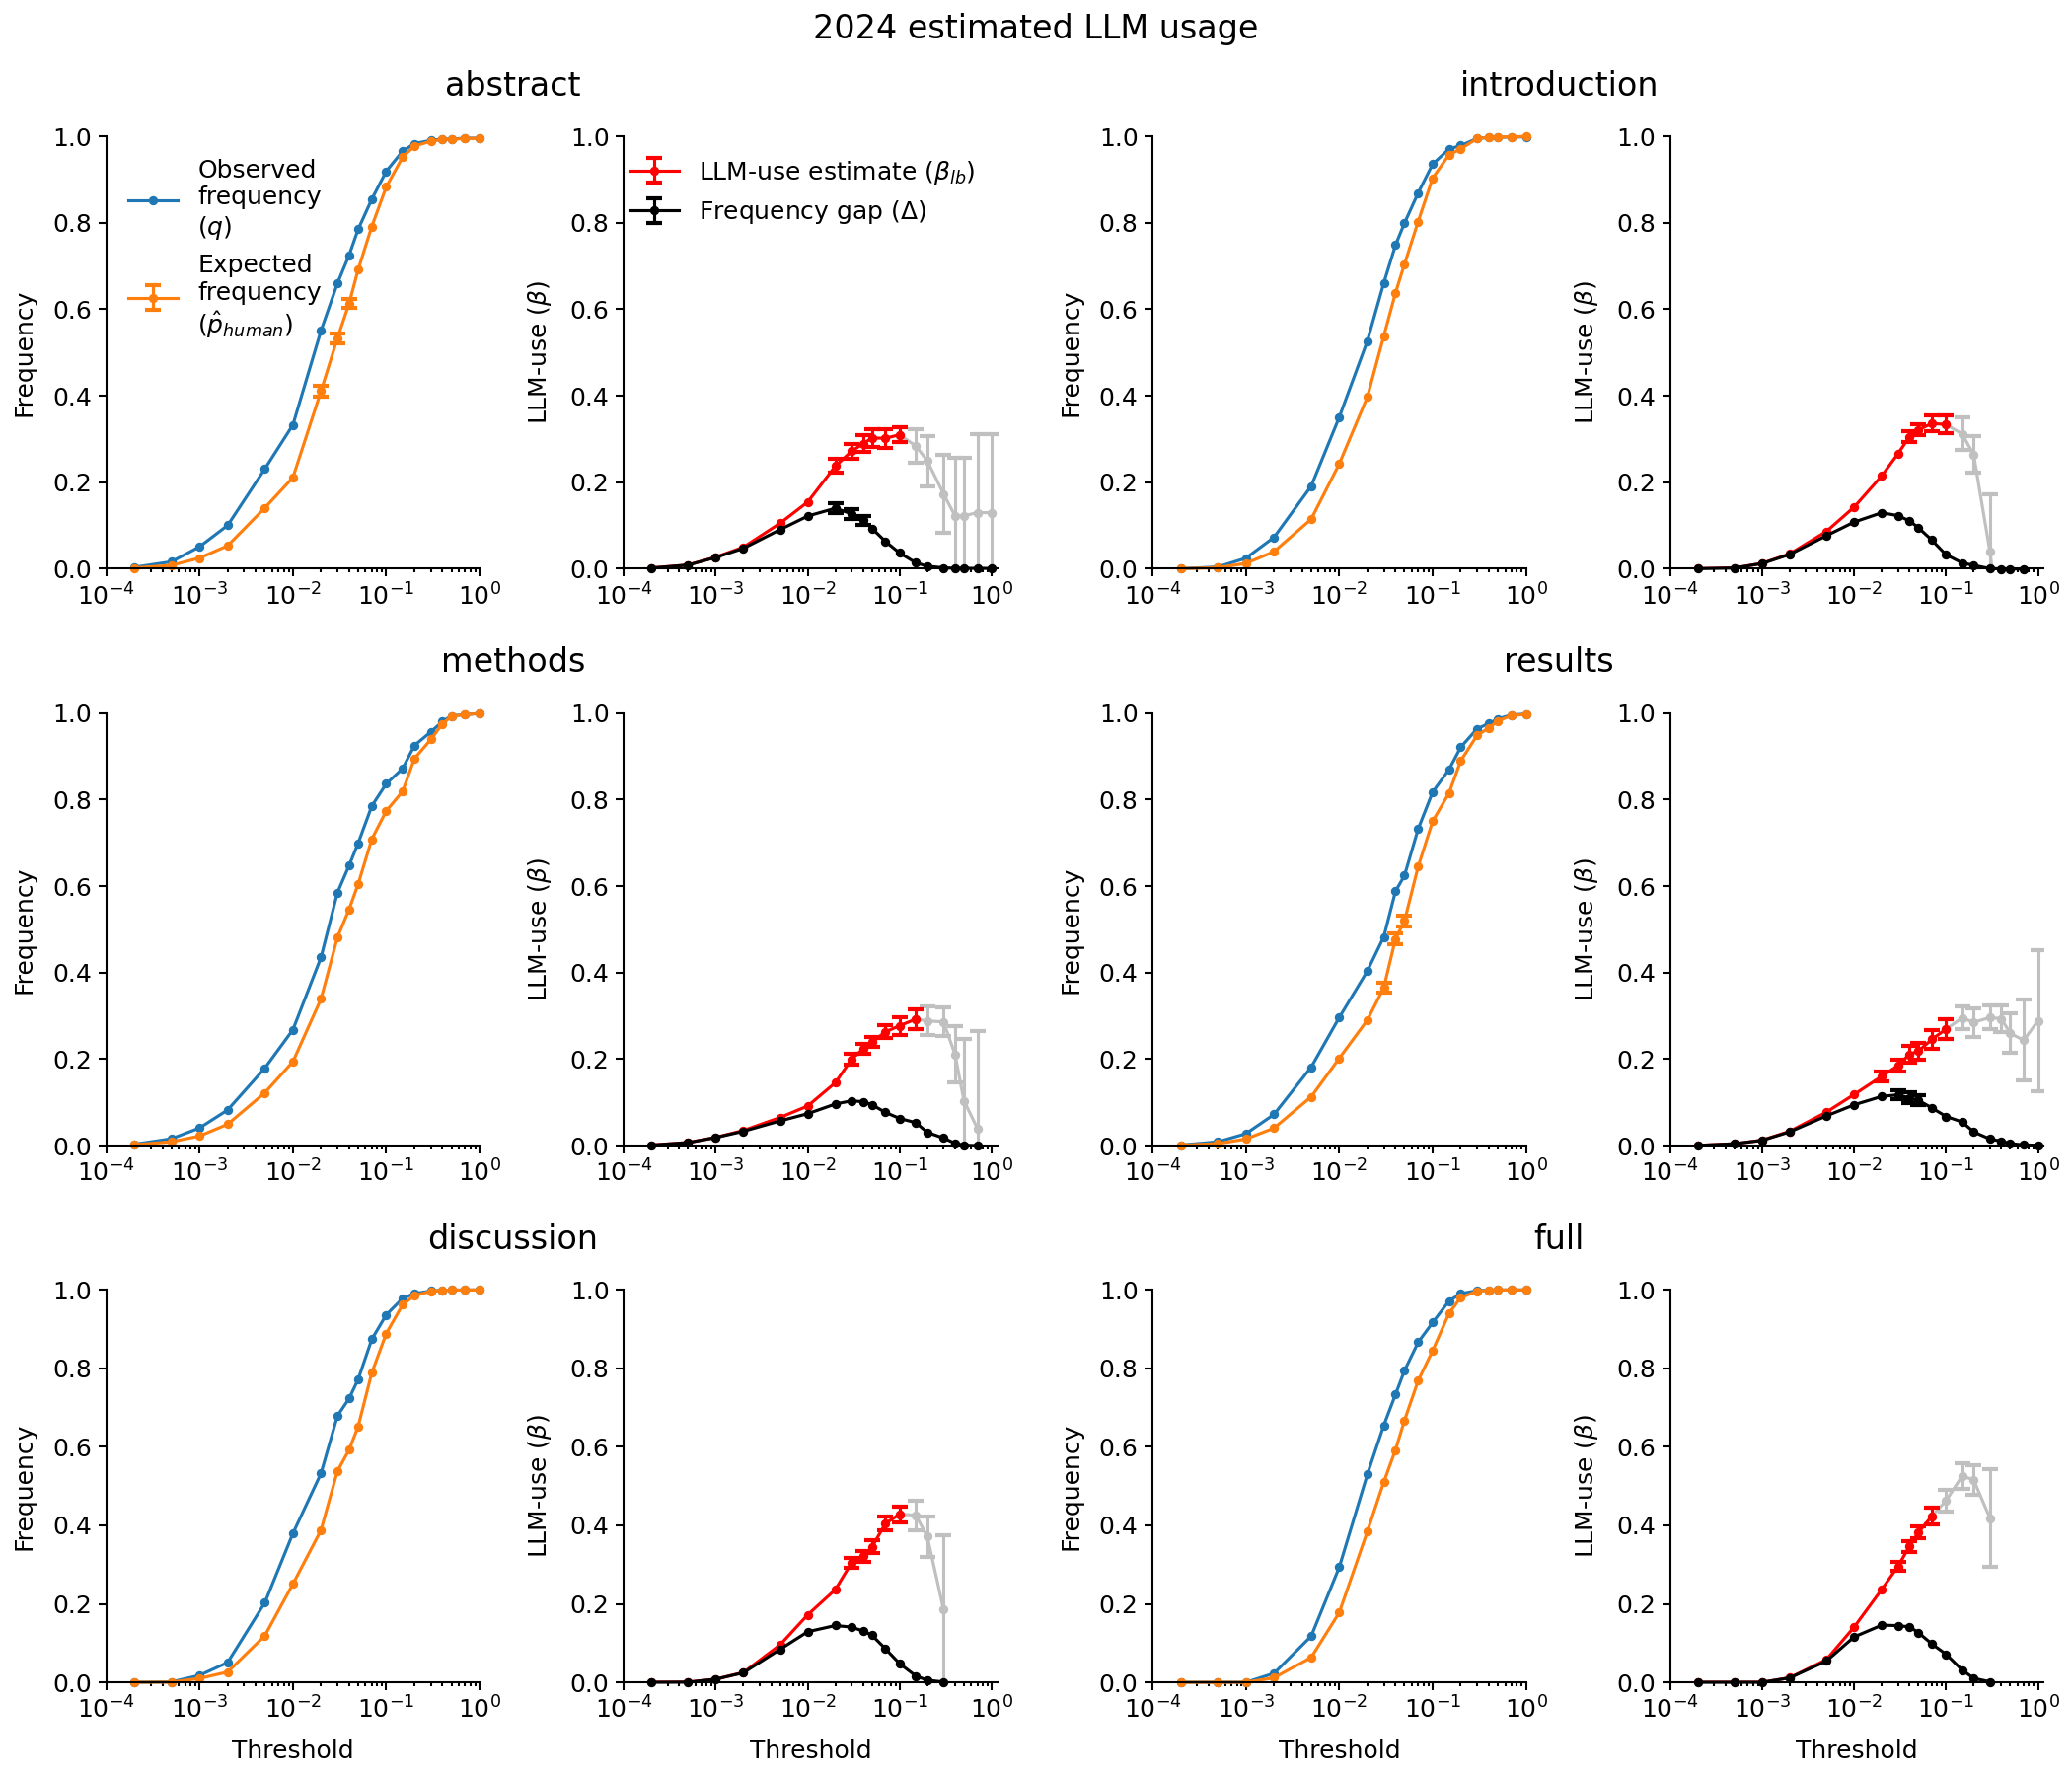
\includegraphics[width=\linewidth]{../results/plots/baseline_2026-01-23/research-article_aimrd_f/5y_2024_lower_bound_non_lemmatized_.png}
    \caption{}
    \label{fig:2024_optimization}
\end{figure}

%comment: add table with -optimal cutoff -length of resulting word list - usage estimate at optimal cutoff for all sections (+crop and sample) and all years
\begin{table}
\begin{tabular}{lrrrrrrrrr}
    \toprule
                & \mcthree{2023} & \mcthree{2024} & \mcthree{2025}\\
                & \mcone{$\hbet$} & \mcone{cutoff} & \makecell[c]{excess\\words}& \mcone{$\hbet$} & \mcone{cutoff} & \makecell[c]{excess\\words} & \mcone{$\hbet$} & \mcone{cutoff} & \makecell[c]{excess\\words} \\
    \midrule
    abstract        & 0.09 \unc{0.02} & 0.10 & 355 & 0.31 \unc{0.02} & 0.10 & 355 & 0.53 \unc{0.01} & 0.10 & 355 \\
    introduction    & 0.12 \unc{0.02} & 0.10 & 324 & 0.34 \unc{0.02} & 0.07 & 307 & 0.50 \unc{0.02} & 0.07 & 307 \\
    methods         & 0.11 \unc{0.02} & 0.15 & 348 & 0.29 \unc{0.02} & 0.15 & 348 & 0.46 \unc{0.02} & 0.15 & 348 \\
    results         & 0.09 \unc{0.02} & 0.10 & 325 & 0.27 \unc{0.02} & 0.10 & 325 & 0.47 \unc{0.02} & 0.15 & 338 \\
    discussion      & 0.14 \unc{0.02} & 0.10 & 297 & 0.43 \unc{0.02} & 0.10 & 297 & 0.68 \unc{0.01} & 0.10 & 297 \\
    full            & 0.12 \unc{0.02} & 0.05 & 211 & 0.42 \unc{0.02} & 0.07 & 232 & 0.77 \unc{0.02} & 0.20 & 296 \\
    \bottomrule
\end{tabular}
\end{table}


\section{Subgroup analysis}
\subsection{Countries and language regions}

\begin{figure}[htbp]
    \centering
    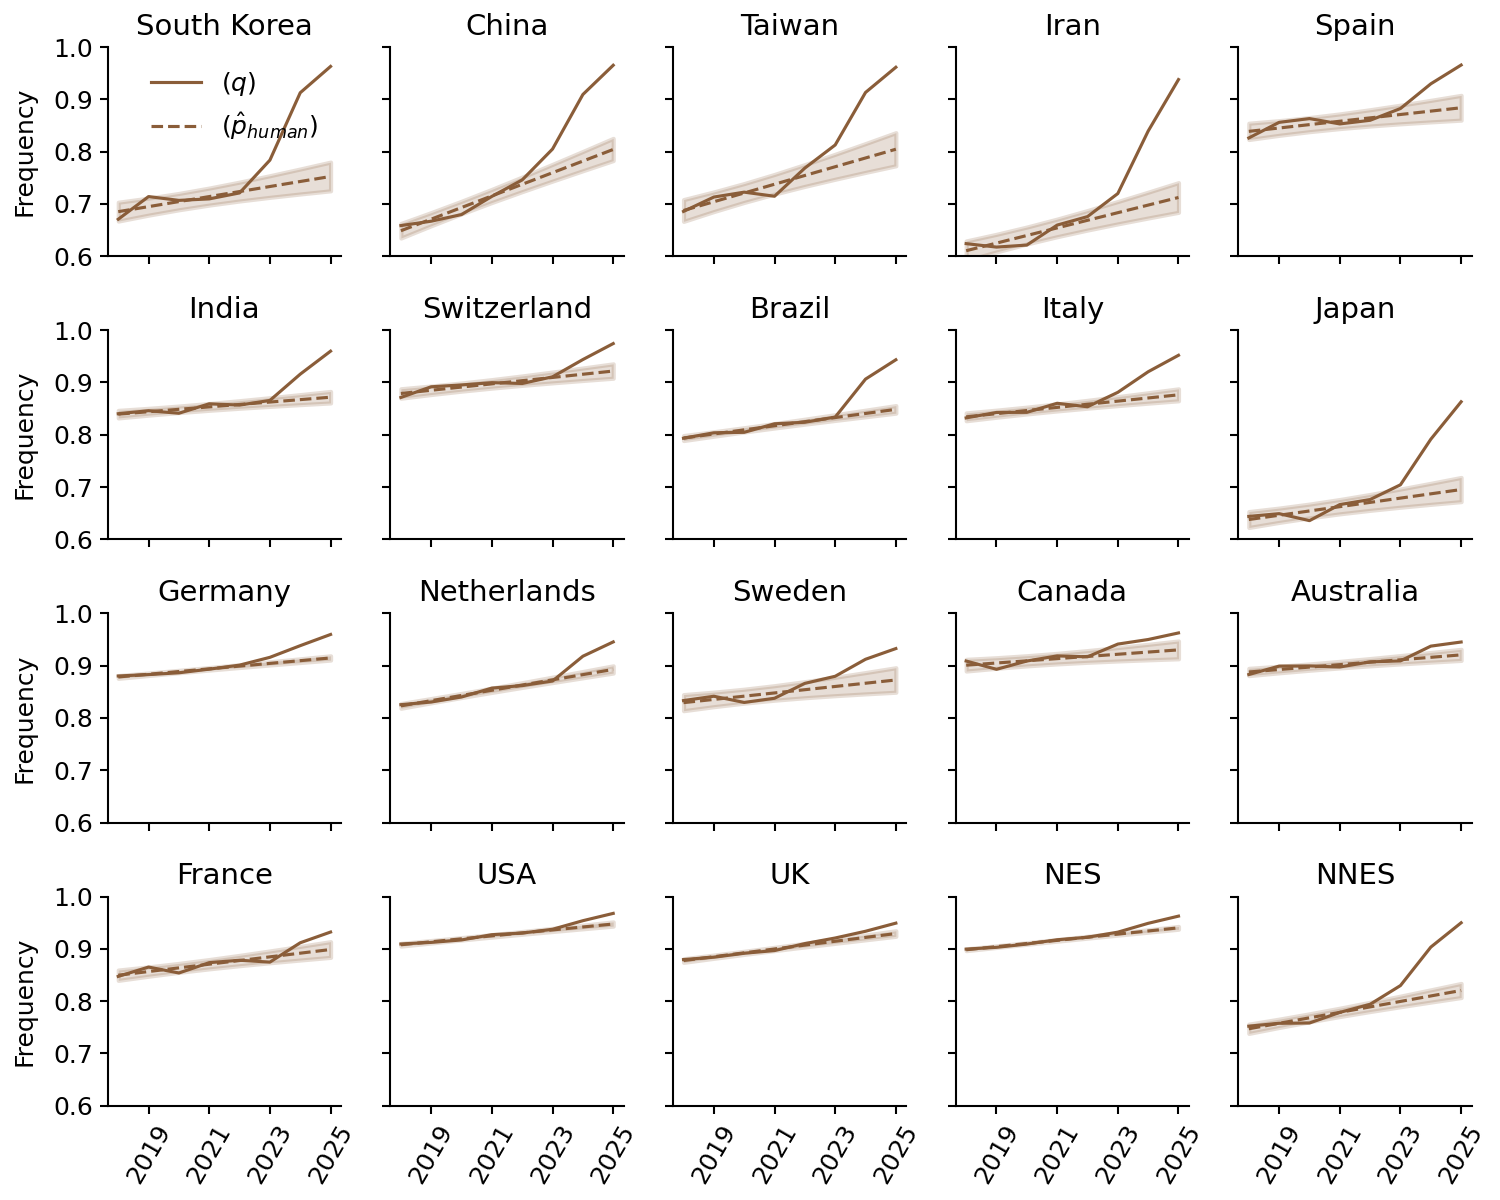
\includegraphics[width=\linewidth]{../results/plots/baseline_2026-01-23/research-article_aimrd_f/countries_individual_freqs_subsubopt.png}
    \caption{}
    \label{fig:countries_freqs}
\end{figure}

\subsection{Academic Discipline}\label{ap:disciplines}

\begin{figure}[htbp]
    \centering
    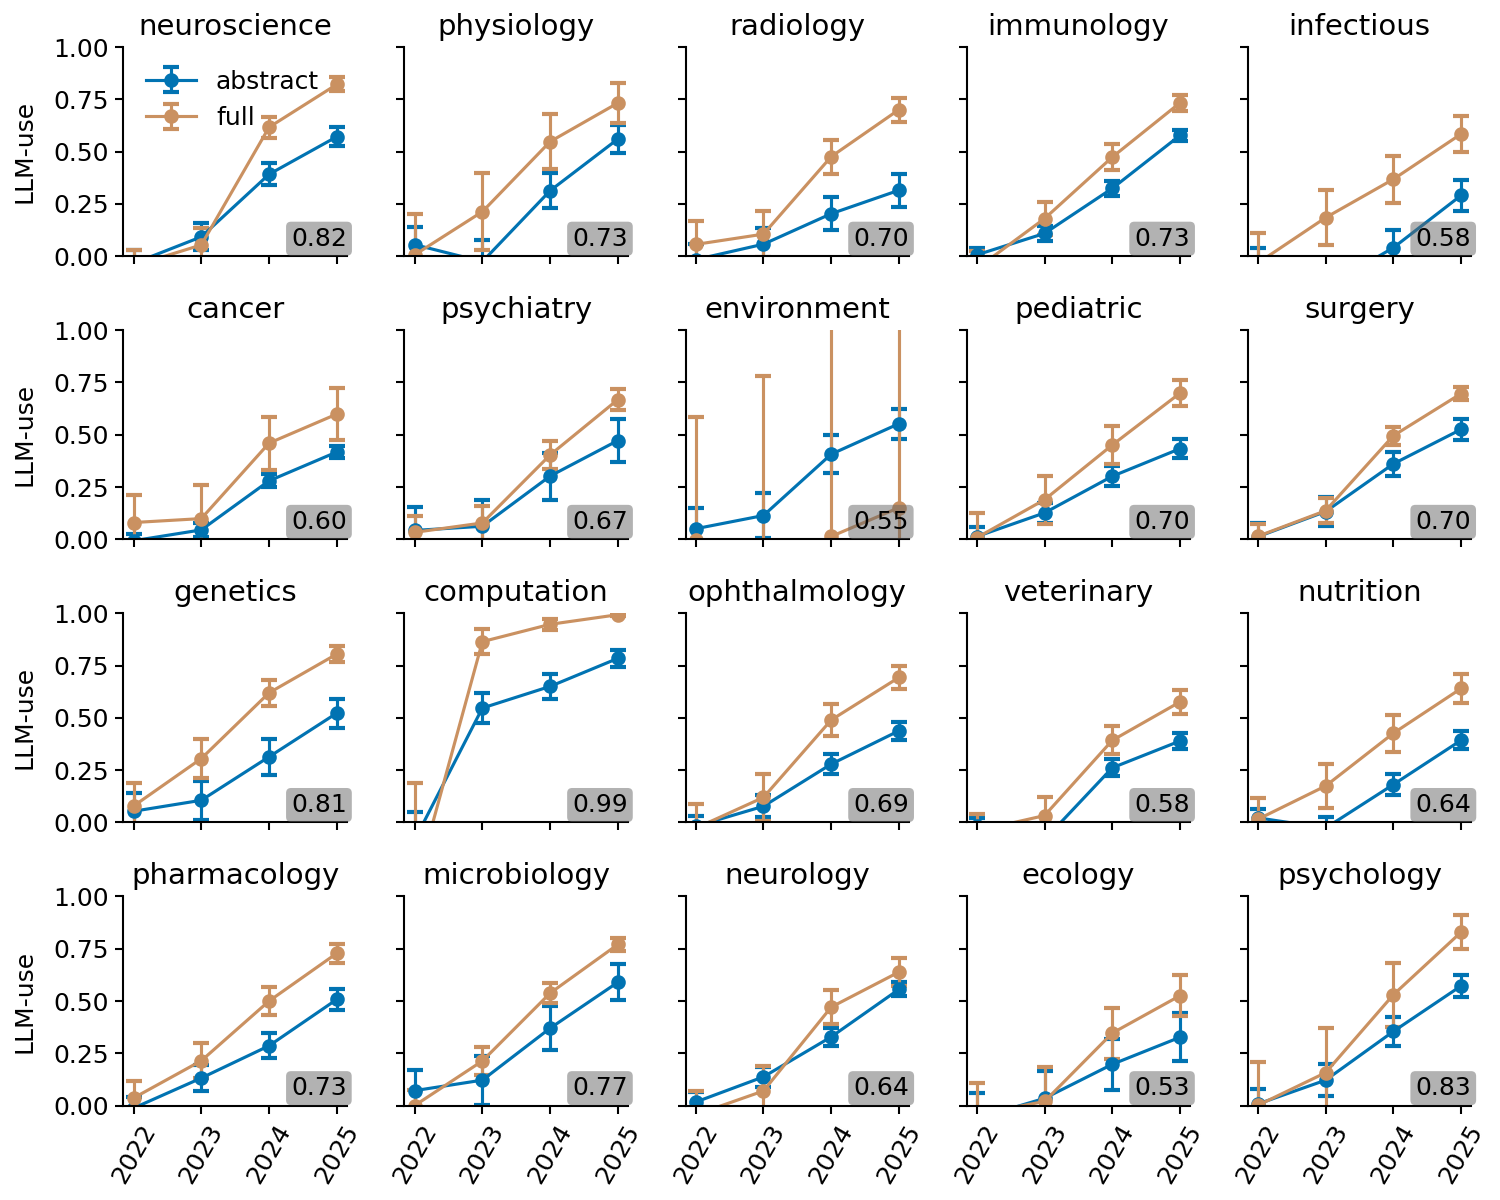
\includegraphics[width=\linewidth]{../results/plots/baseline_2026-01-23/research-article_aimrd_f/disciplines_individual.png}
    \caption{LLM-use estimates for different academic disciplines contributing to PMC for the abstract and main body of the paper. The highest estimate in each panel is marked in a gray box.}
    \label{fig:disciplines_ind}
\end{figure}

\begin{figure}[htbp]
    \centering
    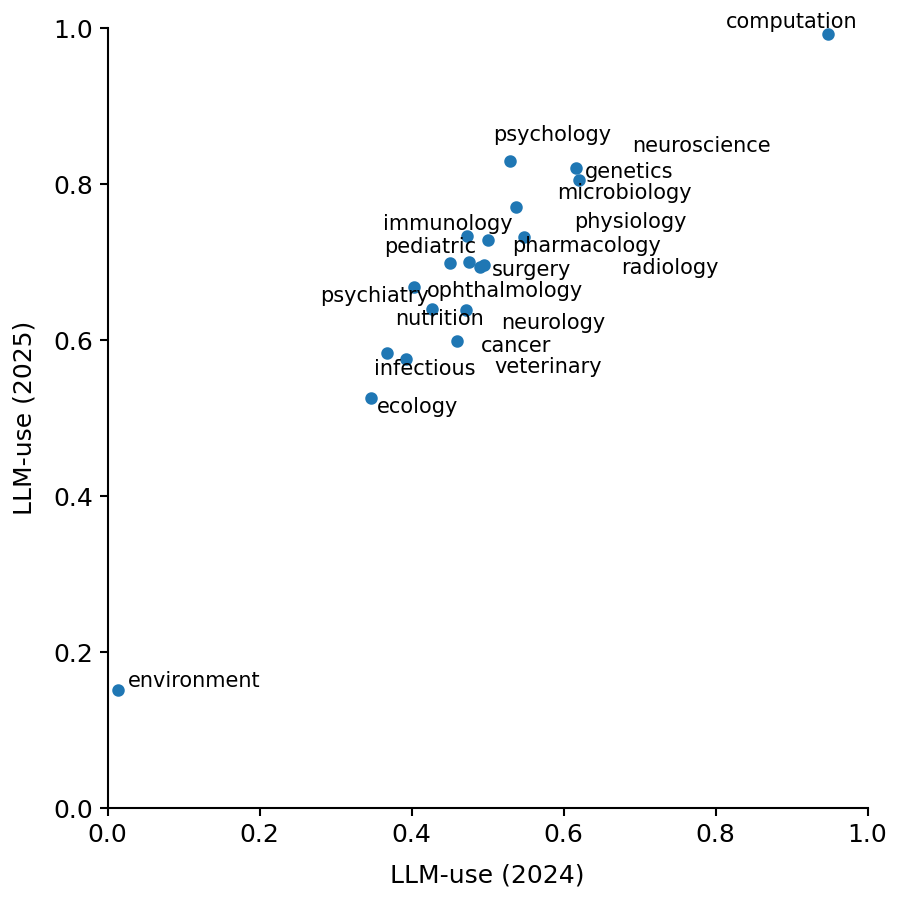
\includegraphics[width=\linewidth]{../results/plots/baseline_2026-01-23/research-article_aimrd_f/disciplines_2024v2025.png}
    \caption{LLM-use estimates of 2024 (x-axis) and 2025 (y-axis) for different academic disciplines. Because the number of papers in each category is very small, some estimates have very high uncertainty.}
    \label{fig:disciplines_all}
    %comment: this should be a different color than countries
\end{figure}

\end{document}


%\documentclass{article}
%\usepackage{settings}

%\title{LLM-use in biomedical publications - an estimation}
%\author{Lena Holzwarth}
%\date{March 2026}

%\addbibresource{references.bib} %Import the bibliography file

%\begin{document}
%\maketitle

%\section{Introduction}\label{sec:intro}

Since the release of OpenAI's ChatGPT\footnote{https://chatgpt.com/} in November 2022, chatbots based on Large language models (LLMs) have become ubiquitous in the public consciousness.
Due to their continued improvement, going from simple chat interfaces to fully integrated agentic systems like Anthropic's Claude Code\footnote{https://claude.com/product/claude-code}, they are increasingly helpful in any workplace dealing with writing, programming, or project planning.
One such workplace is academia, and it is not surprising that researchers across disciplines have begun to adopt LLMs for editing or writing papers, peer reviews, or grant applications \cite{Kwon2025}.
Proponents of the technology praise it as a tool for accessibility and inclusivity \cite{Bao2025_linguistic, Berdejo-Espinola2023, Prakash2025}, arguing that it enables non-native English speakers (NNES) to overcome language barriers by translating or performing grammar checks \cite{Kousha2025}.
However, the surge of ChatGPT's popularity is accompanied by concerns of misuse \cite{Liebrenz2023, Zheng2023}.
LLMs are prone to hallucination, so if their output is not thoroughly checked before using it in a paper, false or misleading statements might be published, especially if the review is also delegated to an LLM \cite{Alansari2026, Lindsay2023, Walters2023, Xu2025}.
Chatbots also make scientific fraud much easier, with the possibility of fabricating entire papers at the cost of a single prompt \cite{Kendall2024}.  
Reviewers relying on LLMs are vulnerable to hidden prompts in the paper's text, telling the LLM to give a positive review \cite{Lin2025_hidden_prompts}.
In light of these concerns, many journals have issued guidelines about the disclosure of LLM-use \cite{Brainard2023}. 
However, the perception of LLM-use leading to inaccuracies in the text, together with journals restricting or explicitly banning certain use-cases may incentivize academics against disclosing \cite{Thorp2023}.
Consequently, when trying to investigate the prevalence of LLM-use in academia, and especially in the paper-writing process, relying on self-disclosure statements will lead to underestimation \cite{Kousha2024, Kwon2025}.
\\
Regardless of the ethical concerns about using LLMs as paper-writing assistants, their prolonged use in academic text production will have an impact on academic writing as a whole.
LLMs have a distinct writing style.
Sentences generated by them have been shown to be less diverse in length \cite{Desaire2023}, but to have higher lexical diversity and positive sentiment \cite{Mak2025}.
Famously, they also show a preference for certain words, an observation which has lead to much ridicule around the most popular example ``to delve'' \cite{MacClure2024}.
The reason for this behavior is not entirely clear.
Juzek and Ward \cite{Juzek2025} replicated the training process of chatbots and tried to artificially create word preferences in the model.
They found no evidence to suggest that the training data, model architecture, or training algorithm have an influence in forming these idiosyncratic word choices.
However, the authors were able to induce an LLM with preferred words during reinforcement learning with human feedback (RLHF), the continued training scheme behind the success of modern Chatbots \cite{Bai2022}.
During RLHF, humans provide learning goals by rating the interaction with the model.
For commercial Chatbots, this work is often performed by precariously employed workers in the global south, for example in Nigeria, where ``delve'' is used much more frequently than in other English-speaking countries \cite{Perrigo2023, Hern2024}.
\\
These selective word preferences can be leveraged to estimate the proportion of LLM-processed text in a corpus.
Kobak et al. \cite{Kobak2025} track changes in word frequencies in biomedical abstracts from the PubMed database.
They compare a word's observed frequency in a given year with a projection based on its frequencies two and three years back.
The metric obtained by subtracting the predicted from the observed frequency is called excess frequency: A change in frequency that diverges from previous trends.
They identify many words that appear with excess frequency in abstracts from 2024.
This is notable, because for previous years, the observed frequency gaps are much smaller.
Because of that, a threshold can be applied to excess frequency, such that most words from pre-2024 don't exceed it, but many from 2024 do.
In addition, the majority of pre-2024 excess words are clearly related to a specific research topic, such as ``ebola'' in 2015, ``convolutional'' in 2017, or ``coronavirus'' in 2020.
In contrast, many excess words in 2024 are content-independent style words -- ``underscore'', ``potential'', ``significant'' or ``pivotal'', to name just a few.
The qualitative and quantitative differences between excess words from before and after 2024 point to a drastic shift in writing patterns that can only be explained by the adoption of LLMs into the writing process.
The identified excess style words for 2024 can therefore be interpreted as marker words for LLM-use.
It's important to note that the marker words should be applied to analyses on the corpus level and not to individual documents -- one ``delve'' does not an LLM-generated text make. 
While these words appear more frequently in LLM outputs, some of them still have very low frequency in both human and machine text.
There are texts by human authors that include them, and LLM-generated texts that don't.
\\
Using the combined excess frequencies of a selection of excess style words, Kobak et al. derive a lower bound for LLM-use estimates.
Their reasoning is quite intuitive: all instances of using one of the relevant words that go beyond the predicted frequency must have been caused by LLM-use.
Excess frequency as a metric has the advantage of not needing to distinguish between using an LLM write a whole paragraph, or suggesting changes on previously written text.
Both use-cases will lead to some LLM-suggested words being present in the final product.
\\
Here, we expand on their work on excess word frequency as a lower bound estimate of LLM-use in biomedical abstracts by making the following contributions:
\begin{itemize}
    \item \textbf{Widening the focus} from an analyzing only the abstract to the entire paper. By using the open-access PubMed Central (PMC \cite{pmc}) dataset  instead of PubMed, the proportion of LLM-assisted text in the main text of the paper can be compared with usage in the abstract, and different sections within the body can be compared against each other. 
    \item Deriving a \textbf{stronger lower bound} metric going beyond excess frequency. We show that while excess frequency is an intuitive estimate for LLM-use, it severely underestimates the true proportion of LLM-assisted text. 
    \item Computing \textbf{uncertainty measures} and performing tests on \textbf{simulated data} to increase confidence in the estimates. A disadvantage of the previous approach is the lack of a ground-truth set to test performance with. By simulating the data generation process in a Binomial model of word occurrence, we can evaluate our metric for several ground-truth levels of LLM-use.
    \item \textbf{Comparing} the LLM-use estimates with those of other estimation approaches, as well as survey data asking researchers about their LLM-use. Unlike previous studies, we find that LLM-like language has almost completely permeated academic writing.
\end{itemize}

This thesis is structured in the following way: In Section \ref{sec:related}, other approaches to estimate LLM-use in academia are discussed, such as comparable word frequency measures, word distribution modeling and LLM-detectors.
Section \ref{sec:methods} gives an overview of the data processing pipeline, the metrics used to estimate LLM-use, as well as the validation procedure employed to increase confidence in the estimates attained.
This is followed by Section \ref{sec:results}, where our estimates are reported and compared to results from other work.
Finally, the results, along with their impact and limitations are discussed in Section \ref{sec:discussion}.
\\
All code is available on GitHub\footnote{https://github.com/LenaHolzwarth/llms\_in\_academia}.
%The PMC dataset can be downloaded here\footnote{https://ftp.ncbi.nlm.nih.gov/pub/pmc/deprecated/oa\_bulk/}.
%\chapter{Related Work}\label{sec:related}

Since the wide-spread proliferation of LLMs, many techniques to identify traces of LLM-use have been suggested.
As this work is focused on LLM-use specifically in academic writing, the approaches detailed here have been selected accordingly with no claim of exhaustiveness.

\section{Word frequency measures}
Most closely related to our method, word frequency measures make use of the distinct word choices separating LLM and human text production.
While not immediately visible in individual samples, these patterns emerge when looking at word distributions on the corpus level.
Reports of certain words appearing with disproportionate frequency after the introduction of ChatGPT in November 2022 have been made for publications from a wide array of scientific disciplines, ranging from linguistics \cite{Botes2025} or astronomy \cite{Astarita2024}, to medicine \cite{Matsui2024} or dentistry \cite{Uribe2024}.
\\
These observations of increased word frequency can be used to derive estimates for the prevalence of LLM-use in a given corpus, using the words with the most pronounced frequency changes as markers.
For example, Gray \cite{Gray2025} computes the relative yearly change of word frequency in papers from the Dimensions database, both for single words and word groups of up to twelve terms.
The terms are selected from a list of LLM marker words identified by Liang et al. \cite{Liang2024_review}.
Their LLM-use estimate is based on the frequency change of these excess words or word groups.
The word frequencies of 2022 are multiplied with the highest frequency increase between two consecutive pre-ChatGPT years to obtain a conservatively estimated counterfactual baseline of human word frequency. 
The number of papers with at least one of the marker words in 2023 exceeding the amount explained for by the baseline divided by the total number of papers serves as their LLM estimate.
A later study from the same author repeats the same procedure with an updated word list \cite{Gray2025}, following reports that some marker words showed decreased usage in 2024, making them less useful as LLM-use markers \cite{Geng2025}.
\\
Kousha and Thelwall \cite{Kousha2025} employ a similar approach of monitoring frequency changes of marker words in abstracts from Scopus, Web of Science and PubMed, as well as full papers from PMC, Dimensions and OpenAlex.
They select some of the marker words reported in previous research, followed by collecting additional marker words by searching for words with high co-occurrence with the pre-selected list.
While they observe strong increases in marker word frequency between the years 2022 and 2024, they don't use this to estimate the prevalence of LLM-use in their data.
However, based on their results, Gray \cite{Gray2025} derives an estimate by comparing the frequency of the word "underscore" in observed 2022 directly to its frequency in 2024 (not taking into account that human usage of the word is also subject to yearly changes).

\section{Word distribution modeling}\label{subsec:freq_model}
Similarly to the approaches detailed in the previous section, word distribution modeling makes use of distinctive word frequency patterns in LLM-generated text.
However, instead of relying only on observed frequencies in the target corpus, they model word frequencies in scientific writing as a mixture distribution of human-written and LLM-assisted text.
\\
Using a technique they call ``distributional GPT quantification'', Liang et al. \cite{Liang2024_review} analyze peer reviews of AI conference papers.
Their work is based on the observation that the fraction of LLM text in the sample can be estimated via maximum likelihood estimation (MLE) on the corpus, if the probability distributions for human and LLM-generated text are known. 
The probability distribution for human text can be estimated by counting word occurrence in texts from pre-LLM years.
To obtain the probability distribution of words in LLM-generated text, the authors prompt ChatGPT to generate alternative reviews of the conference papers from before 2023.
The authors model the distribution of all adjectives instead of relying only on marker words associated with LLM-use.
As a validation of their method, a corpus with a known fraction of LLM-generated text was constructed by sampling from the original and generated reviews. 
By computing the MLE for this corpus, the researchers are able to retrieve the correct proportion.
\\
The authors apply the same method to abstracts and introductions of scientific papers sourced from arXiv, bioRxiv and Nature portfolio journals \cite{Liang2024_paper, Liang2025}. 
LLM text is sampled by tasking ChatGPT to create a summarization outline of a paragraph from an existing, pre-ChatGPT paper, which is then given to the LLM with a prompt to generate a full paragraph based on this outline.
\\
A slightly different method is introduced by Geng and Trotta \cite{Geng2024}, who investigate LLM-use in arXiv abstracts.
Like the previous approach, they base the human word frequency baseline on pre-2023 papers and LLM frequency baseline on outputs from ChatGPT asked to polish or re-write pre-2023 abstracts.
Then, they compute a word's frequency change rate by comparing its frequencies in the original and rewritten abstracts.
The authors argue that estimates derived from a word list are more robust than those derived from single words, and further claim that the choice of the word list yielding the most accurate estimate depends on the (unknown) underlying value of LLM-use.
To find the optimal word list for each of a set of ground-truth LLM-use values to validate their procedure, they create test data with a fixed proportion of original and LLM-edited abstracts.
For each ground-truth LLM-use value, a word list is created by optimizing thresholds on word frequency and frequency change rate.
Combining the observed frequency with the simulated frequency change rate, they can derive different estimates for LLM-use in the real data using all word lists.
The mean of the estimates is taken as the preliminary result.
The estimates are then repeated with the three word lists optimized for the LLM-use proportions closest to the preliminary result.
\\
The validation procedure with ground-truth LLM-generated text is a marked advantage of these studies, compared to the frequency-based estimates, where no validation set with known distribution is available. 
However, this validation is strongly dependent upon the exact model and prompt that were used to create the LLM corpus.
The estimated distribution based on this corpus might differ drastically from the true LLM distribution, which is likely to have been created from a multitude of prompts and models.
To illustrate this point, Geng and Trotta perform validations on papers edited with a minimally different prompt than the one used to derive the frequency change rate, which leads to a systematic overestimation of true LLM-use.
While the true value is still within the error bounds, stronger alterations to the prompt or the use of a different model are likely to have a stronger impact on the estimates.

\section{LLM-detectors}
A more fine-grained approach to observing or modeling word distributions across entire corpora is to train classifiers on identifying LLM-use in individual texts. 
\\
\textbf{Zero-shot LLM detection} or model self detection uses properties of the model's idiosyncratic text generation process to determine how likely it is for a text sample to have been generated by the LLM.
An early example of this approach is \textbf{GLTR} \cite{Gehrmann2019}, which determines for every word in the text which ranking it has among the LLM's suggestions given its position in the text.
The lower the average ranking of the selected words, the more likely it is for the text to have been written by a human author.
\textbf{Detect-GPT} \cite{Mitchell2023} uses a separate LLM to generate perturbed versions of the sample and computes the log-likelihood of the original and perturbed versions under the target model. The log-likelihood of a text sample generated by the target LLM will be higher than that of the perturbed variants, while the same is not true for human-written text.
\textbf{Binoculars} \cite{Hans2024} uses a similar approach by normalizing the perplexity of a sample text under one model by the cross-perplexity of the re-generation of the sample text by a different model.
The perplexity is the negative log-likelihood of a text and can be thought of as the model's surprise, i.e. how far the text diverges from something the model would have produced. 
Binoculars has been used to check papers from the preprint platforms arXiv, bioRxiv and medRxiv \cite{Cheng2024}.
The disadvantage of these approaches is two-fold: First, in order to classify a piece of text, one needs to know with which LLM it was potentially generated, and second, one needs access to the scoring function of the LLM. 
While this is possible for some GPT variants, the scores of the most widely used model, ChatGPT, are not open to the public \cite{Mitchell2023}.
Also, these methods assume the whole text to be LLM generated, which would impede their accuracy on samples that were only partially edited with LLMs.
\\
\textbf{Trained LLM detectors} rely on a training corpus of ground-truth LLM and human text.
As an alternative to zero-shot detection, they circumvent the need for access to model parameters and can, in theory, work model-agnostically, if the training set is constructed with samples from different models.
Their performance is, however, critically dependent on the prompts and models used to generate the training corpus \cite{Liu2024_profiles}.
A common approach is to fine-tune a pretrained language model to distinguish between LLM-generated and human-written text.
Another possibility is to train conventional classifiers such as XGBoost or support vector machines on embedded representations of training text \cite{Bao2025_classifier}.
\textbf{Feature-based detectors} use linguistic features, such as the variation in sentence length, as indicators of LLM-use \cite{Desaire2023}. 
The classifier is then trained not on the texts themselves but on the features extracted from them.

There is also a plethora of proprietary LLM detectors on the market (some of which are free-to-use).
Most of them don't disclose their model architecture or training procedure.
Because of their relative convenience, many researchers investigating LLM-use in academia opt for these models to generate estimates \cite{Akram2024, Liu2024_profiles, Picazo-Sanchez2024}.
Among the models used are originality AI\footnote{https://originality.ai/}, GPTzero\footnote{https://gptzero.me/}, zeroGPT\footnote{https://www.zerogpt.com/}, GPTKit\footnote{https://gptkit.ai/}, Smodin\footnote{https://smodin.io/}, Sapling\footnote{https://sapling.ai/ai-content-detector}, Content at scale AI detector\footnote{Renamed to brandwell: https://brandwell.ai/ai-content-detector/} and Writer AI content detector\footnote{This seems to have been discontinued, the link given by the paper using it redirects to a sales pitch for the company's AI agent}.

Many concerns have been raised about current LLM-detectors' lack of accuracy \cite{Doughman2025, Lazebnik2024, Weber-Wulff2023}, going so far as to dispute even the possibility of reliable LLM-detectors \cite{Sadasivan2025}.
Early methods have been found to discriminate against non-native English speakers, disproportionately flagging their work as AI-generated, and to be unable to adjust to slight prompt changes \cite{Liang2023}.

\section{Surveying scientists}
Perhaps the most straightforward approach to evaluating the prevalence of LLM-use in academia is to ask the researchers themselves. 
Several surveys on scientists' use of AI have been conducted by publishing houses \cite{Elsevier2024, Kwon2025, Nordling2023, VanNoorden2023, Wiley2025} and independent researchers \cite{Eppler2024, Liao2024, Mishra2024, Mohammadi2026}.
These studies can be hard to compare because of different sampling pools and phrasing of questions.
An overview of questions asked in each of the surveys can be found in the Appendix \ref{ap:surveys}.
While some researchers also acknowledge the use of LLMs in their papers, the number of published papers crediting ChatGPT or similar models is much smaller than even conservative estimates of actual LLM-use \cite{Kousha2024}, emphasizing the need for anonymous surveys to produce a more accurate picture of researchers' attitudes towards the technology.
For example, in a survey done by Nature, 28\% of respondents reported to have used LLMs to edit their papers, but only 10\% disclosed their AI use \cite{Kwon2025}.

%\section{Methods}\label{sec:methods}
\subsection{Dataset and Preprocessing}
\begin{figure}[htbp]
    %comment: this should be a different color than frequency
    \centering
    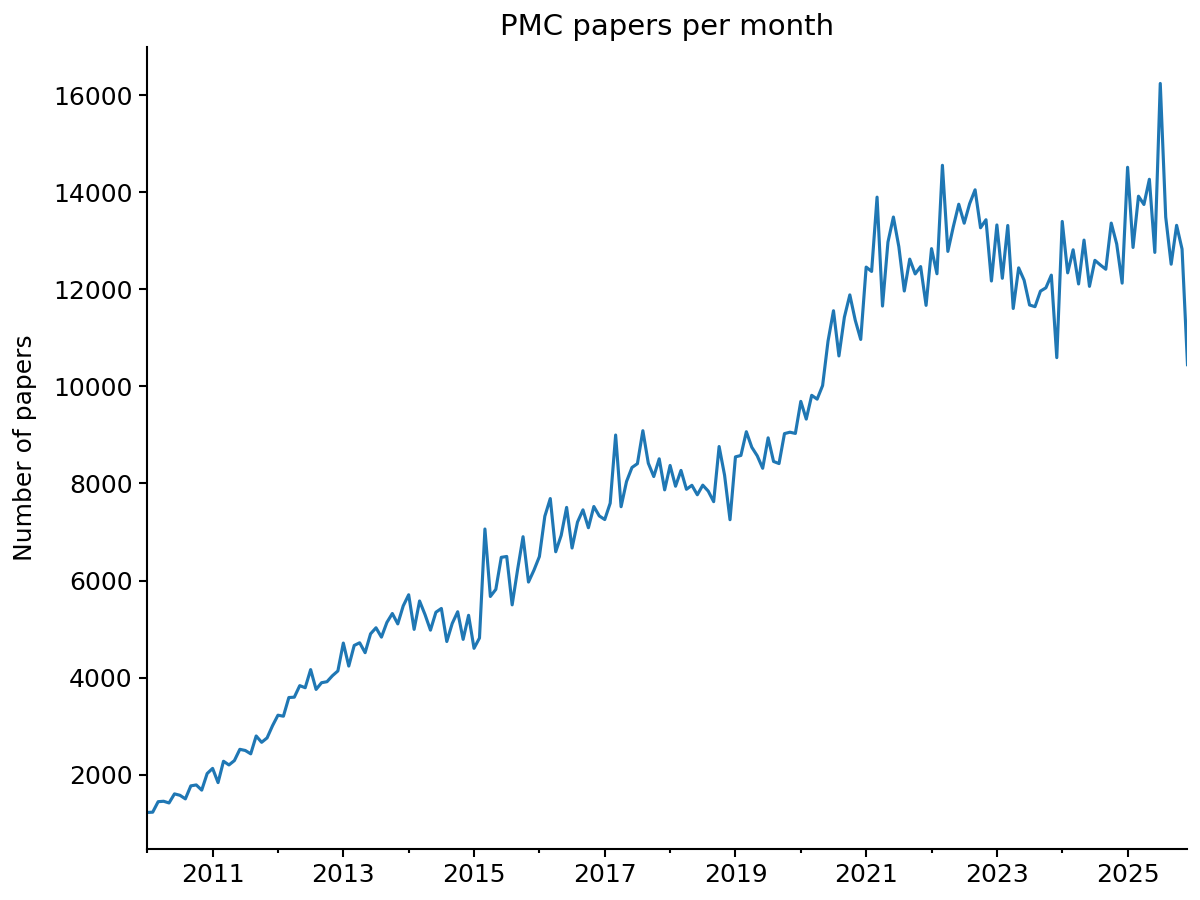
\includegraphics[width=0.7\linewidth]{../results/plots/baseline_2026-01-23/papers_per_month.png}
    \caption{}
    \label{fig:papercount}
\end{figure}
\emph{Pubmed Central}
\\
Pubmed Central (PMC) is a collection of open-access biomedical literature curated by the U.S. National Institutes of Health's National Library of Medicine \cite{pmc}. 
It provides machine-readable versions of the articles in XML format, which can be accessed individually or downloaded in bulk.
There are three open-access subsets available for bulk download with different licensing: commercial, non-commercial and other.
The latter set includes non-machine readable licenses and was therefore not used.
PMC publishes a baseline twice a year containing all papers in the collection up to shortly before the baseline's release date. 
Incremental updates are published daily in separate files.
When a new baseline is released, the previous baseline and all incremental files are replaced.
Here, we used the baseline published on January 23, 2026 containing papers dated December 31, 2025 and before.\footnote{Since work on this thesis started earlier, initial analyses used the previous baseline released June 26, 2025. These were repeated with the January 2026 baseline, so that everything reported here is based on the newer baseline}
The daily updates published after the baseline were not considered.
\\\\
\emph{XML parsing}
\\
From the XML files in the baseline, each corresponding to one paper, the following information was extracted:
\begin{itemize}
    \item Article type: specifies whether the article is a research paper, a review, a comment, etc.
    \item Date
    \item Language: only specified for a minority of papers, but is inferred later during preprocessing 
    \item Country
    \item PMC-ID: unique identifier for every paper in PMC
    \item PMID: unique identifier for PubMed, not available for every paper in PMC
    \item Journal name
    \item Title
    \item Abstract
    \item Sections
    \item Section titles
\end{itemize}
The sections and section titles are parsed from the main body of the XML file.
In general, individual sections are tagged as sec and assigned a title.
This is important for being able to compare different sections with each other, for which we need as many papers as possible with similar sections.
However, since there is no standardized format for the files, some sections are untitled or there are no section tags at all.
In particular, many files have section names for all sections except the Introduction, or don't embed the Introduction in a separate section tag. 
Therefore, if a file has more sections than section titles, and the first section is unnamed, it is assumed to be the Introduction.
Any other untitled sections are discarded.
Similarly, if there is text at the beginning of the body outside of a sec tag, it is assumed to be the introduction. 
This heuristic is not ideal, because the unnamed text contains abbreviations or keywords instead of the introduction in some cases, but since the Introduction is among the sections this study wants to focus on, it strongly increases the number of usable papers.
\\\\
\emph{Preprocessing}
\\
While some XML files specify the paper's language, this is not the case for the majority.
Since the focus here is on English text, we determine each paper's language using polyglot's detector module.
Every non-English paper is discarded.
The dates of each paper are standardized to DD-MM-YYYY format. 
Some entries only specify the month (e.g. "Feb 2025") or season of the year (e.g. "Fall 2025"), in which case the first of the month or start of the (meteorological) season are used as dates.
Papers without date are removed.
Since we want to compare LLM-use across different sections, it is important to have as many papers with comparable section structure as possible.
To achieve this, in a first step the section names were manually standardized by collecting the most frequent section names and mapping them to their standardized version.
For example, \emph{experimental results}, \emph{findings} and \emph{main results} would be mapped to \emph{results}.
If a paper has multiple sections with the same standardized title, they are concatenated.
For example, \emph{data} and \emph{experimental methods} would first both be renamed as \emph{methods} and then combined into a single \emph{methods} section.
Originally, we planned to investigate different article types and article structures, but in the end we focused only on research articles that have exactly the sections Introduction, Methods, Results, and Discussion, since papers with this article structure were the majority in the dataset.
Conversely, all papers with article types other than \emph{research-article} or with more, fewer or different sections were discarded.
Finally, all sections, including the abstract, were required to have a length of at least 250 characters.
These preprocessing steps reduce the dataset from 7,125,722 to 1,602,404 papers, 1,194,287 of which are dated 2017 or later.
\\
The use of PMC, granting us access to the whole paper, enables an extension on \cite{Kobak2025} in two regards: First, we can compare LLM-usage in the abstract to LLM-usage in the entire body of the paper, and second, we can compare different sections within the body with each other.
For this purpose, all of the analyses detailed in the following subsections were performed on the abstract, the introduction, the methods, the results and discussion of the paper, as well as the full paper, which refers to the four sections from the body without the abstract.

\subsection{Excess Frequency and LLM-use lower bound estimates}

\begin{figure}[htbp]
    \centering
    \begin{minipage}[t]{0.48\textwidth}
        \centering
        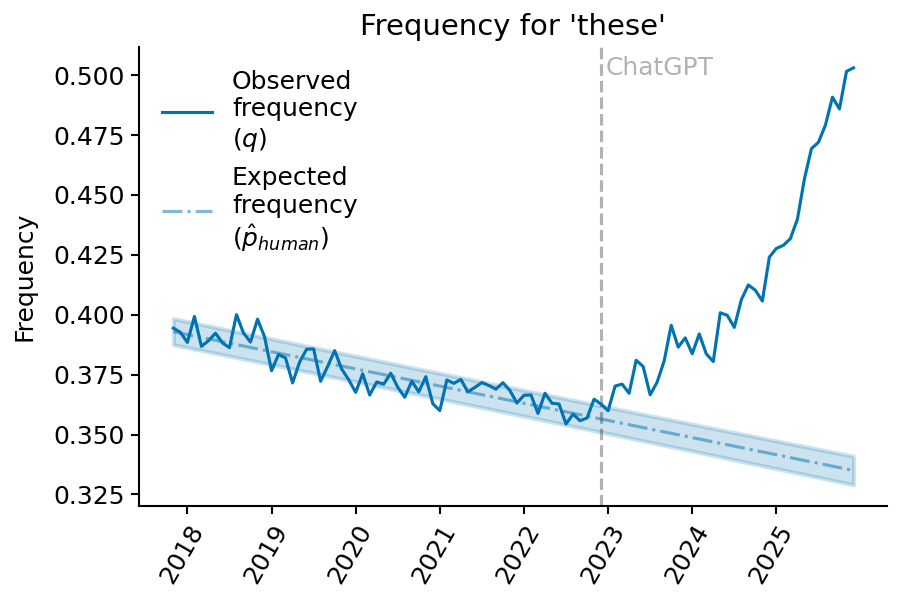
\includegraphics[width=\linewidth]{../results/plots/baseline_2026-01-23/research-article_aimrd_f/these_freqs_time.png}
    \end{minipage}
    \hfill
    \begin{minipage}[t]{0.48\textwidth}
        \centering
        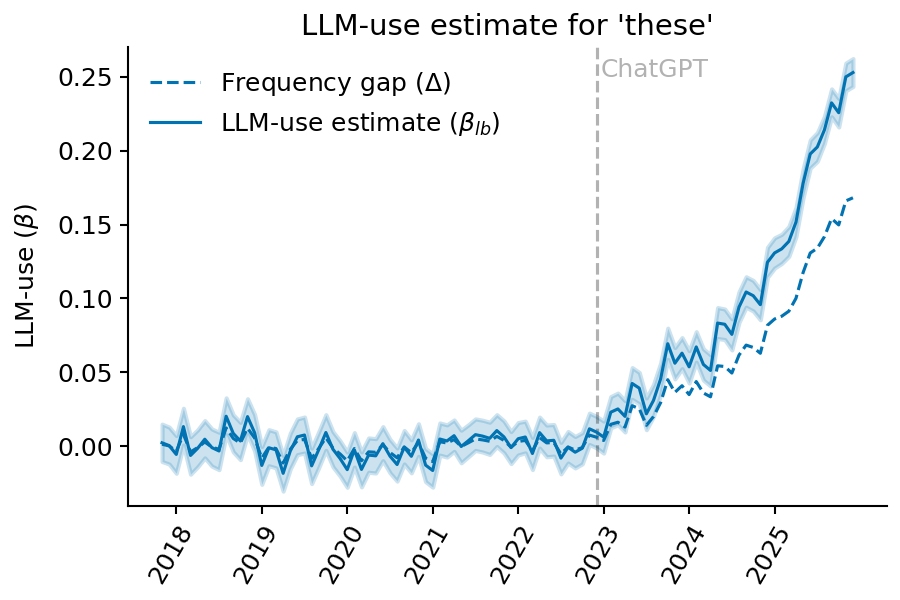
\includegraphics[width=\linewidth]{../results/plots/baseline_2026-01-23/research-article_aimrd_f/these_usage_time.png}
    \end{minipage}
    \caption{Shared caption describing both images}
    \label{fig:two_images}
\end{figure}
Excess frequency, referring to the difference between the observed and predicted frequencies for some word $w$, can be thought of as an intuitive lower bound for LLM use.
To compute it, we first determine the observed frequency of $w$.
We use sklearn's binary CountVectorizer to count the number of papers in each month or year in which $w$ occurs.
Because it is a binary count, it doesn't matter how often $w$ appears in each paper.
The vectorizer only considers words with 4 or more letters, all of which must be part of the English alphabet.
When counting word occurrence, lemmatization is an important consideration: one has to determine whether to treat different inflections of $w$ as the same or as individual words.
With lemmatization, it makes no difference if a paper contains \emph{delves}, \emph{delved} or \emph{delving}, they are all treated as an instance of \emph{delve}.
It is not immediately clear if lemmatization is helpful in this use-case.
We know from previous studies that LLMs prefer certain words.
This could imply that LLMs use all inflections of a word at a higher frequency, or that it has a strong preference for that word in a specific grammatical context (e.g. third-person singular), while using every other inflection at the same frequency in which they occur in human-written text.
As will be detailed in Section \ref{subsec:wordlist}, for the overall LLM-usage estimates, this does not matter. 
For the plots showing results for individual words, such as Figure, all word variants are included in the counts.
The frequencies are computed by dividing the monthly or yearly counts by the total number of papers in each respective time frame.
On a conceptual level, the observed frequencies $q$ are an estimate for the probability of a positive outcome in the Bernoulli trial of whether a word is present in some paper.
For dates prior to the release of ChatGPT in November 2022, marking the beginning of easily accessible LLMs, $q$ corresponds to the frequency of a word in human-written text, $p_{human}$.
After the widespread availability of Chatbots, the observed word frequency can be thought of as the product of a mixture distribution between the probability of a word to appear in human-authored and LLM-assisted text, respectively: 
\begin{equation}
    q = 
    \begin{cases}
        p_{human} & \text{for papers before 11-2022}\\
        (1-\beta) \cdot p_{human} + \beta \cdot p_{LLM} & \text{for papers after 11-2022}\\
    \end{cases}
\end{equation}
The mixture component $\beta$ in the lower case indicates the proportion of papers that were written with the help of LLMs.
We can transform this equation to obtain an expression for $\beta$:

\begin{equation}\label{eq:beta}
\begin{split}
    q &= (1-\beta) \cdot p_{human} + \beta \cdot p_{LLM}\\
    \beta \cdot (p_{LLM}-p_{human}) &= q -  p_{human}\\
    \beta &= \frac{q -  p_{human}}{p_{LLM}-p_{human}}
\end{split}
\end{equation}
\\
While $p_{human}$ can be estimated by the observed $q$ in the time span before November 2022, there is no direct way to do so after the release of ChatGPT.
However, if we assume that human usage of words follows linear trends and is independent of LLM-use, we can use the values before 2022 to model $\hph$ using linear regression.
Since we are interested in both the monthly and yearly trends, we fit the regression either on the five yearly frequency values from 2018 to (including) 2022, or on the 60 monthly frequencies from November 2017 to October 2022.
For the yearly data we include 2022 in the train set because, considering the time it takes to write a paper, and the time it took the new technology to gain traction, it is unlikely that many papers published in December 2022 were written with the help of LLMs.
Replacing the unknown $p_{human}$ with the estimate $\hph$ in equation \ref{eq:beta}, one issue remains: there is no direct way to estimate $p_{LLM}$ from the observed frequencies.
The others solve this problem by using ground-truth LLM-generated text to determine $p_{LLM}$.
Here, we choose a different approach by determining a lower bound for $\beta$ that doesn't rely on $p_{LLM}$:
\begin{equation}\label{eq:delta}
    \begin{split}
        \beta &= \frac{q -  \hph}{p_{LLM}-\hph}\\
        \beta &\ge q - \hph =\Delta
    \end{split}
\end{equation}
This is the excess frequency measure introduced by \cite{Kobak2025} and denoted $\Delta$.
Intuitively, if a word appears in $70\%$ of papers in 2025, but we predict humans to use this word in only $60\%$ of instances, the $10\%$ gap must be accounted for as having been written by LLMs. 
Note that this metric will lead to a strong under-estimation of the actual LLM usage, because a human-use frequency of $60\%$ will only translate to $60\%$ of observed use, if all texts in the sample are in fact written by humans ($\beta=0$).
In reality, some papers were written with the help of LLMs, such that the fraction of word-occurrence that can be explained by human usage is not $60\%$ of all papers, but $60\%$ of the papers with human authorship.
A stronger lower bound, denoted $\hbet$ is also possible:
\begin{equation}\label{eq:beta_hat}
    \begin{split}
        \beta &= \frac{q -  \hph}{p_{LLM}-\hph}\\
        \beta &\ge \frac{q -  \hph}{1-\hph} = \hbet
    \end{split}
\end{equation}
In dividing by $1-\hph$, this lower bound readjusts the estimate by focusing only on the fraction of papers for which no human use of the word is to be expected.
In the above example with $p_{human}=60\%$ and excess frequency of $\Delta=10\%$, $1-\hph=40\%$ of papers wouldn't contain the word if there were no LLM-authored texts, but only $1-q=30\%$ actually don't, so the remaining $\frac{10\%}{40\%}=25\%$ must be LLM-authored.  

\begin{figure}[htbp]
    \centering
    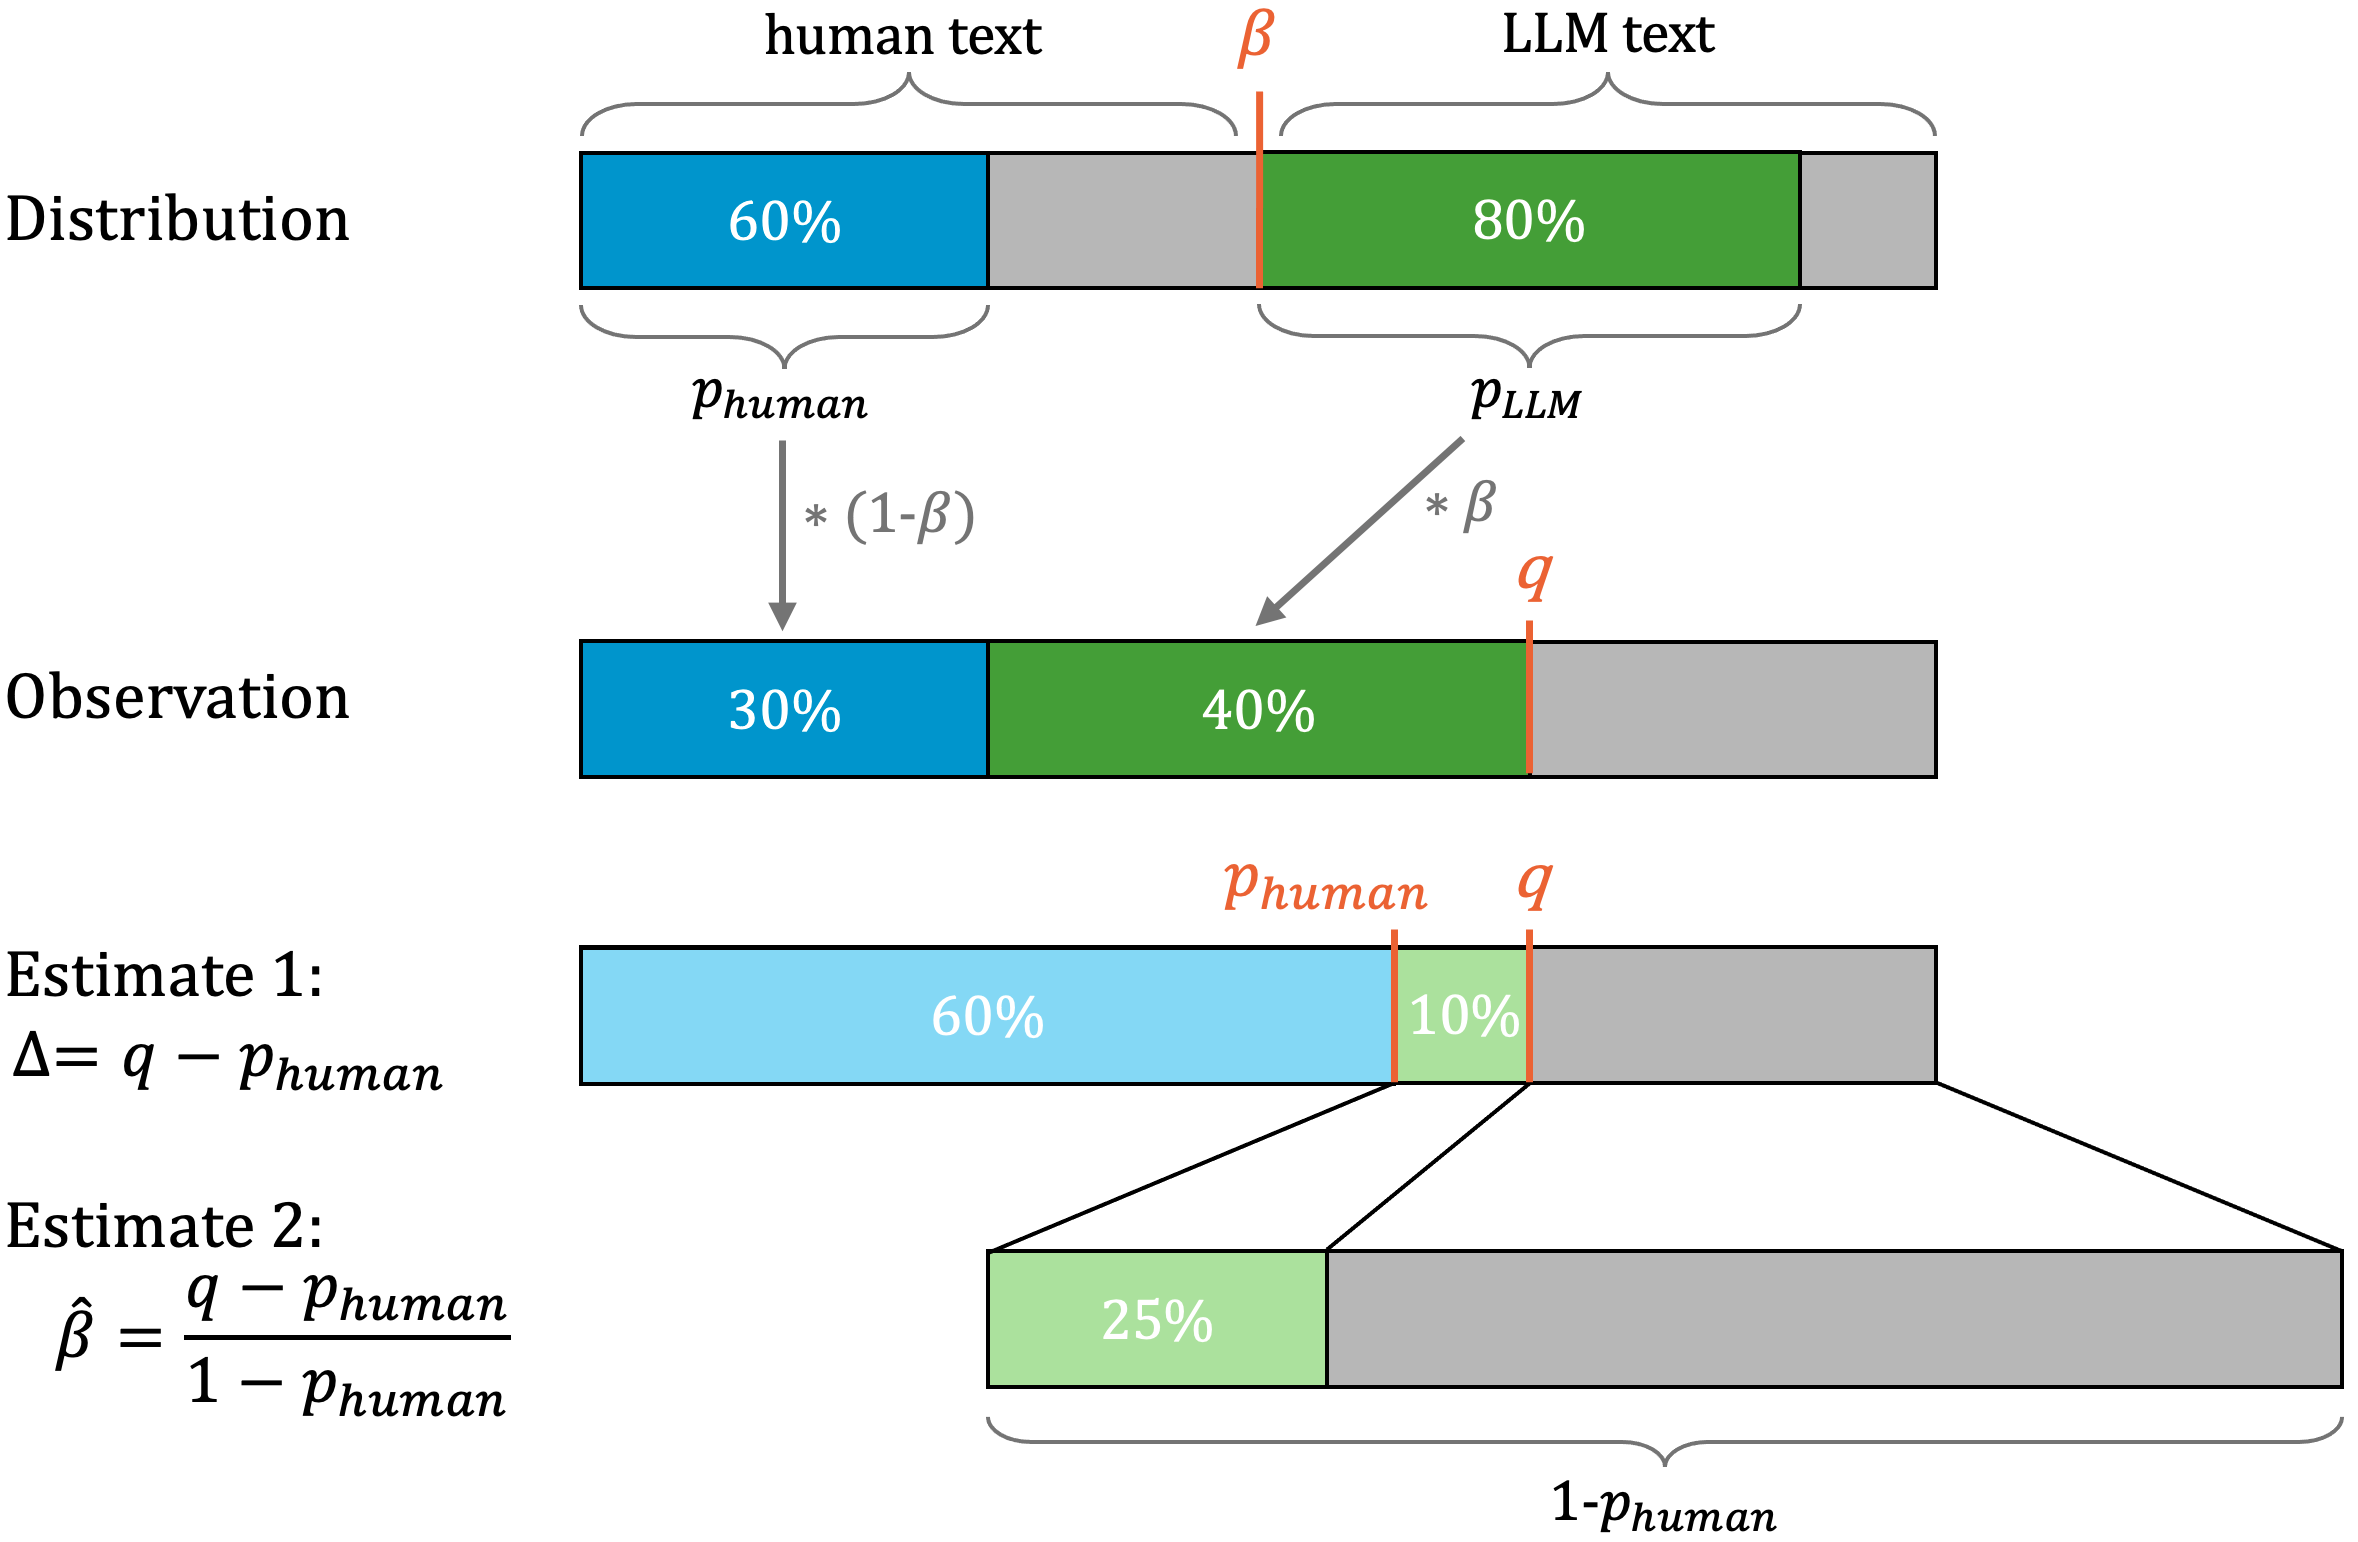
\includegraphics[width=0.7\linewidth]{../results/plots/misc/intuition_estimate_v2.png}
    \caption{}
    \label{fig:intution_estimates}
\end{figure}



\subsection{Grouped word frequencies}\label{subsec:wordlist}
\begin{figure}[htbp]
    \centering

    \begin{minipage}[t]{0.48\textwidth}
        \centering
        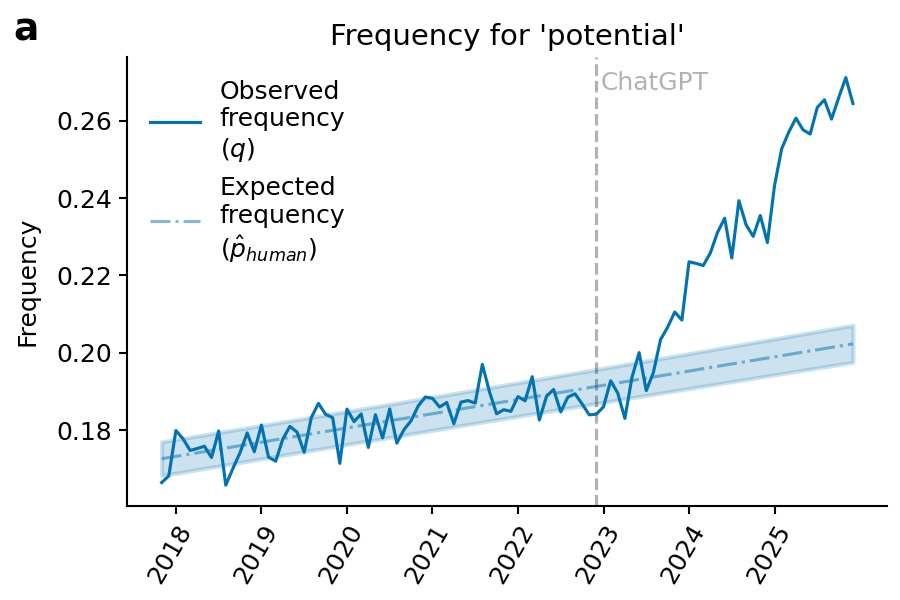
\includegraphics[width=\linewidth]{../results/plots/baseline_2026-01-23/research-article_aimrd_f/potential_freqs_time.png}
    \end{minipage}
    \hfill
    \begin{minipage}[t]{0.48\textwidth}
        \centering
        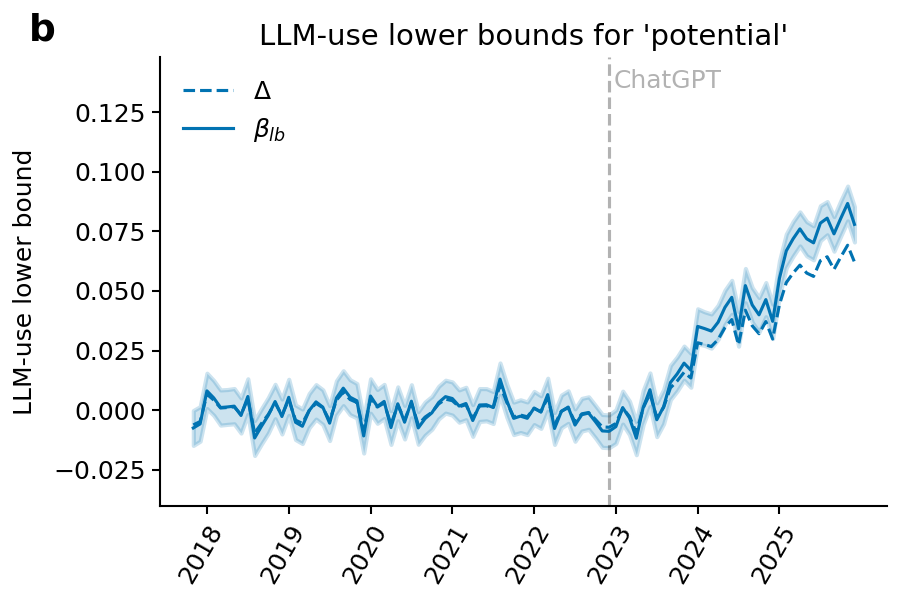
\includegraphics[width=\linewidth]{../results/plots/baseline_2026-01-23/research-article_aimrd_f/potential_usage_time.png}
    \end{minipage}

    \medskip

    \begin{minipage}[t]{0.48\textwidth}
        \centering
        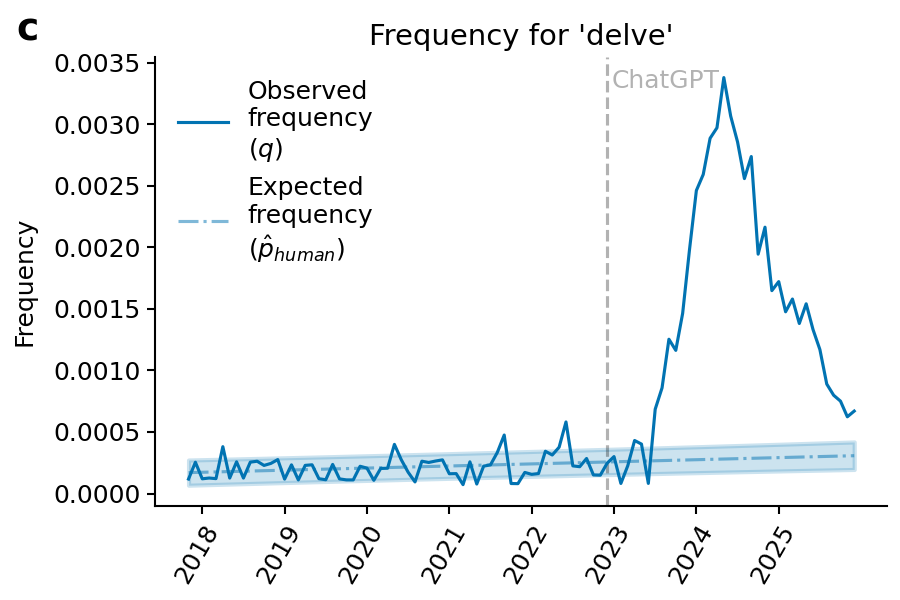
\includegraphics[width=\linewidth]{../results/plots/baseline_2026-01-23/research-article_aimrd_f/delve_freqs_time.png}
    \end{minipage}
    \hfill
    \begin{minipage}[t]{0.48\textwidth}
        \centering
        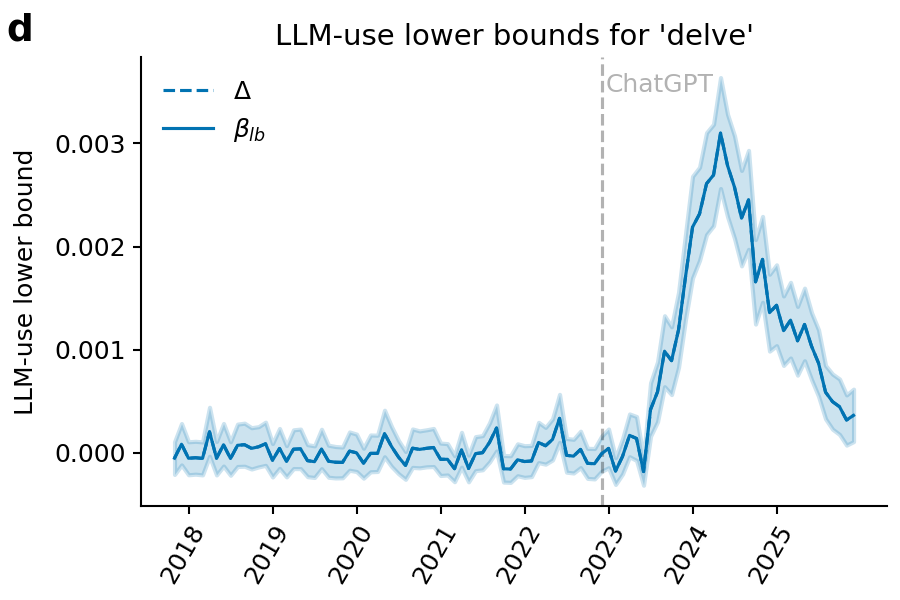
\includegraphics[width=\linewidth]{../results/plots/baseline_2026-01-23/research-article_aimrd_f/delve_usage_time.png}
    \end{minipage}

    \caption{Fix title for delve estimates!}
    \label{fig:four_images}
\end{figure}

While single words are useful to illustrate the concept of excess frequency, they are suboptimal as a basis for an accurate estimate of overall LLM-use.
The reason for this is obvious: while LLMs might use a word such as ``potentially'' at a higher frequency than humans would, ``potentially'' doesn't fit in every context so there will potentially be a lot of LLM texts not containing it.
Also, the observed frequencies of some words might be unreliable.
The word ``delve'', used as the titular example of excess vocabulary in \cite{Kobak2025}, has experienced a sharp decline in popularity starting around mid-2024, when it was widely reported as an example of ``LLM-speak''.
Many authors have thus moved to using word lists as markers. 
The method of computing the frequencies doesn't change, but instead of counting in how many papers a single word appears, we count in how many papers at least one of the words in the list appears.
The most systematic way to create a list of words indicative of LLM-use is to use a data-driven approach, which doesn't require a manually selected list.
\\\\
\emph{Excess words for 2024 PubMed}
\\
\cite{Kobak2025} determine the excess words for 2024 by computing the frequency gap and the frequency ratio for each word in their dataset.
The frequency gap is the same metric as $\Delta$ in Equation \ref{eq:delta}, although they only use the yearly frequencies of 2021 and 2022 to predict $\hph$.
The frequency ratio is computed as $\frac{q}{\hph}$.
An excess word is defined as any word with frequency gap or frequency ratio above a certain threshold.
The thresholds were chosen in such a way that the majority of words in texts from the years 2012 - 2023 were excluded
(The gaps for previous years were also computed by comparing observed values to $\hph$ computed based on two and three years prior).
Using both metrics as inclusion criteria serves to increase the number of excess words.
For instance, a word whose usage increases from 0.0001 to 0.001 will have a relatively small gap but a large ratio, while a word whose prior frequency of 0.3 rises to 0.4 has a large gap with a relatively small ratio. 
Both changes mark a notable difference in usage and should therefore be candidates for marker words.
All words above the threshold were then manually annotated as \emph{style words} or \emph{content words}.
\emph{Content words} are all words related to the research topic of a certain paper. 
Their excess use can be attributed to new inventions or research trends.
Examples include ``RNN'' in 2018, ``Covid'' in 2020, and ``ChatGPT'' in 2024.
\emph{Style words}, on the other hand, are not related to research topics and could be found in any discipline: ``these'', ``potentially'', ``delve'', etc.
Excess words of 2024 were defined as all style words with frequency gap or ratio gap above the respective thresholds.
This resulted in a list of 379 words, which can be found in the Appendix \ref{ap:wordlist}.
\\\\
\emph{Optimal word lists}
\\
The excess word list can be used to create the optimal list of marker words to detect LLM-use.
It might be counter-intuitive to not just use the whole list: if any of the words can act as a marker for LLM-use, then using as many words as possible should yield the most accurate result.
However, one has to keep in mind that all excess words also appear in human-written text.
If there are too many words in the list, their cumulative frequency will be close to 1 even for $p_{human}$.
For \cite{Kobak2025}, who use the frequency gap $\Delta$ as their LLM-use estimate, this is suboptimal because the closer $\hph$ is to 1, the smaller the potential gap.
When using $\hbet$ as the metric, the best estimate would be achieved by getting $p_{LLM}$ as close to 1 as possible, which would in turn move $\hbet$ closer to the true value $\beta$.
While $p_{LLM}$ isn't observable, it can be manipulated by increasing the number of words in the excess list.
However, this also includes the caveat that $\hph$ must remain smaller than 1, otherwise, Equation \ref{eq:beta_hat} yields division by zero.
This means that for both estimates, $\Delta$ and $\hbet$, a subset of the 2024 excess words needs to be determined.
Because brute-forcing the decision on an optimal list by trying all possible combinations is not feasible, \cite{Kobak2025} sorted the excess words by their individual frequencies in 2024 (lowest to highest), and then used different cutoff values to create subsets of all words whose individual frequencies were below the cutoff. 
Each resulting list was used to compute the LLM-use estimate $\Delta$ and the highest $\Delta$ was used as the final estimate.
\\\\
\emph{Adaptation to PMC data}
%comment: include graph of excess words for one section? also include the paper composition?
Initially, we planned to repeat the procedure of finding excess words for the PMC dataset.
This turned out to be non-feasible, because the length of the full papers, as opposed to only abstracts, lead to a huge number of excess words, which would all have to be manually annotated to filter them for style words.
Instead, we used the previous study's 2024 excess word list.
This is permissible because, first, PMC is a subset of the PubMed data used in \cite{Kobak2025}, so the domain is similar, and second, the point of using style words is to have marker words that are domain-independent.
(Although it is likely that when searching for excess words in a different domain, such as news articles, the resulting list would be somewhat different).
The 2024 excess word list is not lemmatized, so that ``delving'' and ``delves'' are treated as different words.
Since we are not interested in the excess words on a semantic level and use them only as indicator of LLM use, it does not matter if two words on the list are variations of the same verb, or if a third variation of the verb is not included.
To get the optimal list for each section, we sort the 2024 excess words by their individual frequency in 2024.
This leads to a somewhat different order for each section.
Like in the previous work, we then use different cutoff values to create subsets of excess words, which serve as a basis for computing the LLM-use estimate $\hbet$.
We started with x cutoffs spaced evenly on a log-scale between 0 and 1 and later added intermediate values in the high-interest region around the maximum, resulting in y cutoffs.
Initially, we used the same approach as above to select the maximum $\hbet$-value as the estimate.
However, in some cases, the maximum was at one of the highest cutoff value, leading to nearly the full excess word list being used for the estimate.
This results in values for $q$ and $\hph$ that are extremely close to 1, sometimes with $\hph$ being larger than $q$, which contradicts the assumption $p_{human} < p_{LLM}$.
As a consequence, both numerator and denominator of the fraction $\frac{q - \hph}{1-\hph}$ are very close to 0, which can lead to unstable behavior.
To prevent this, any cutoff that leads to estimates of $\hph \ge 0.999$ was excluded as candidate for creating optimal excess word lists.
%comment: check this number and include plot that shows oscillation of estimates that go too close to 1
\\
The optimization was performed on yearly frequency data separately.
This means that the optimal cutoff for 2024 could be different to that of 2025.
For the main analysis, the optimal cutoff values for 2025 were used for all time points to simplify procedure and have more easily comparable results.
Notably, the main analysis was performed on monthly data with the word lists optimized for the year 2025, instead of optimizing each month individually, for simplicity.
A possible approach with optimizing on monthly intervals of the data would be to take the majority optimum as the list for all estimates.
The end result would be the same: Some time intervals would be estimated with the optimal word list, while others wouldn't.
\\
To better judge the reliability of the estimates, we computed the standard error and performed sanity checks using simulated frequency data.

\subsection{Method validation}
\emph{Standard error for LLM-use estimates}
Since the LLM-use estimate $\hbet=\frac{q -  \hph}{1-\hph}$ depends on $\hph$ and $q$, we first need to determine their respective errors, before propagating them to obtain the error for $\hbet$.
We conceptualize $q$ as the maximum likelihood estimate (MLE) for the binomial probability of a word from the excess word list to appear in a paper.
As such, the MLE's variance is $SE_q^2=\frac{q(1-q)}{n}$, with $n$ as the number of papers in the current month or year.
$\hph$ is the regression estimate of a binomial probability. 
Since $\hph$ is not an empirical estimate, the binomal MLE variance doesn't apply and we focus on the regression variance.
Technically, the data points that the regression was trained on are empirical estimates (since training was done on $q$ values in the time span before the release of ChatGPT).
To factor in this binomial maximum likelihood uncertainty, it should be included in the regression formula.
However, because the MLE variance is very small due to the large number of papers each month, this was omitted for simplicity.
The regression variance for design matrix $X$ (including only points on which the regression is fit, corresponding to the time before the release of ChatGPT), predictor matrix $x$ (including all points that are to be predicted, including pre- and post-ChatGPT frequencies) and response vector $y$ is computed with the following formula:
\begin{equation}
    SE_{\hph}^2= \hat{\sigma}^2 x(X^TX)^{-1}x^T + \hat{\sigma^2}
\end{equation}
with $\hat{b}=(X^TX)^{-1}X^Ty$ as the estimated regression coefficients\footnote{As per common convention, the estimated regression coefficients are normally denoted $\hbet$, which was changed to $\hat{b}$ to avoid confusion with the LLM-use estimate $\hbet$}
and $\hat{\sigma}^2=\frac{\|y-X\hat{b}\|^2}{n-2}$ the unbiased estimate of the noise variance, where $n$ refers to the number of papers, of which the number of predictors, 2, is subtracted.
$\hat{\sigma}^2x(X^TX)^{-1}x^T $ is the covariance matrix of the regression coefficients, specifying the uncertainty of the mean prediction. 
To this, an additional $\hat{\sigma}$-term is added to estimate how far the predicted values would have deviated from this mean.
\\
The variance of $\hbet$, as a nonlinear function of $q$ and $\hph$, is not trivial to determine.
We can apply the Delta method, which uses Taylor series approximation, to do so.
We assume $q$ and $\hph$ to be the means of random variables $Q$ and $P$, respectively.
First, we approximate $\hbet((Q,P))$ around the mean $\mu=(q, \hph)$ with a first-order Taylor expansion:
\begin{equation}
    \hbet((Q,P)) \approx \hbet(\mu) + \nabla\hbet(\mu)^T((Q,P)-\mu)
\end{equation}
with gradient $\nabla$ as
\begin{equation}
    \nabla \hbet(\mu)= \left[ \frac{\partial\hbet}{\partial q}, \frac{\partial\hbet}{\partial \hph}\right]^T = \left[ \frac{1}{1-\hph}, \frac{q-1}{(1-\hph)^2}\right]^T 
\end{equation}
We can use this to compute the variance of $\hbet$:
\begin{equation}
    \begin{split}
        Var(\hbet) &= Var(\hbet(\mu) + \nabla\hbet(\mu)^T((Q,P)-\mu)\\
        &= Var(\hbet(\mu) + \nabla\hbet(\mu)^T(Q,P)-\nabla\hbet(\mu)^T\mu)\\
        &= Var(\hbet(\mu)^T(Q,P))\\
        &= \nabla\hbet(\mu)^T\Sigma\nabla\hbet(\mu)
    \end{split}
\end{equation}
We assume independence of the two random variables $Q$ and $P$, so that the covariance matrix $\Sigma$ only has the diagonal entries of the estimate variances $SE_q^2$ and $SE_{\hph}^2$ derived above. 
We excluded all estimates with a standard error of $SE_{\hbet}\ge 0.025$.
%comment: the error bars don't work if p is 1 (or veryvery close to 1), because in that case, binomial error is 0
\\\\
\emph{Sanity check simulation}
\\
\begin{figure}[htbp]
    \centering
    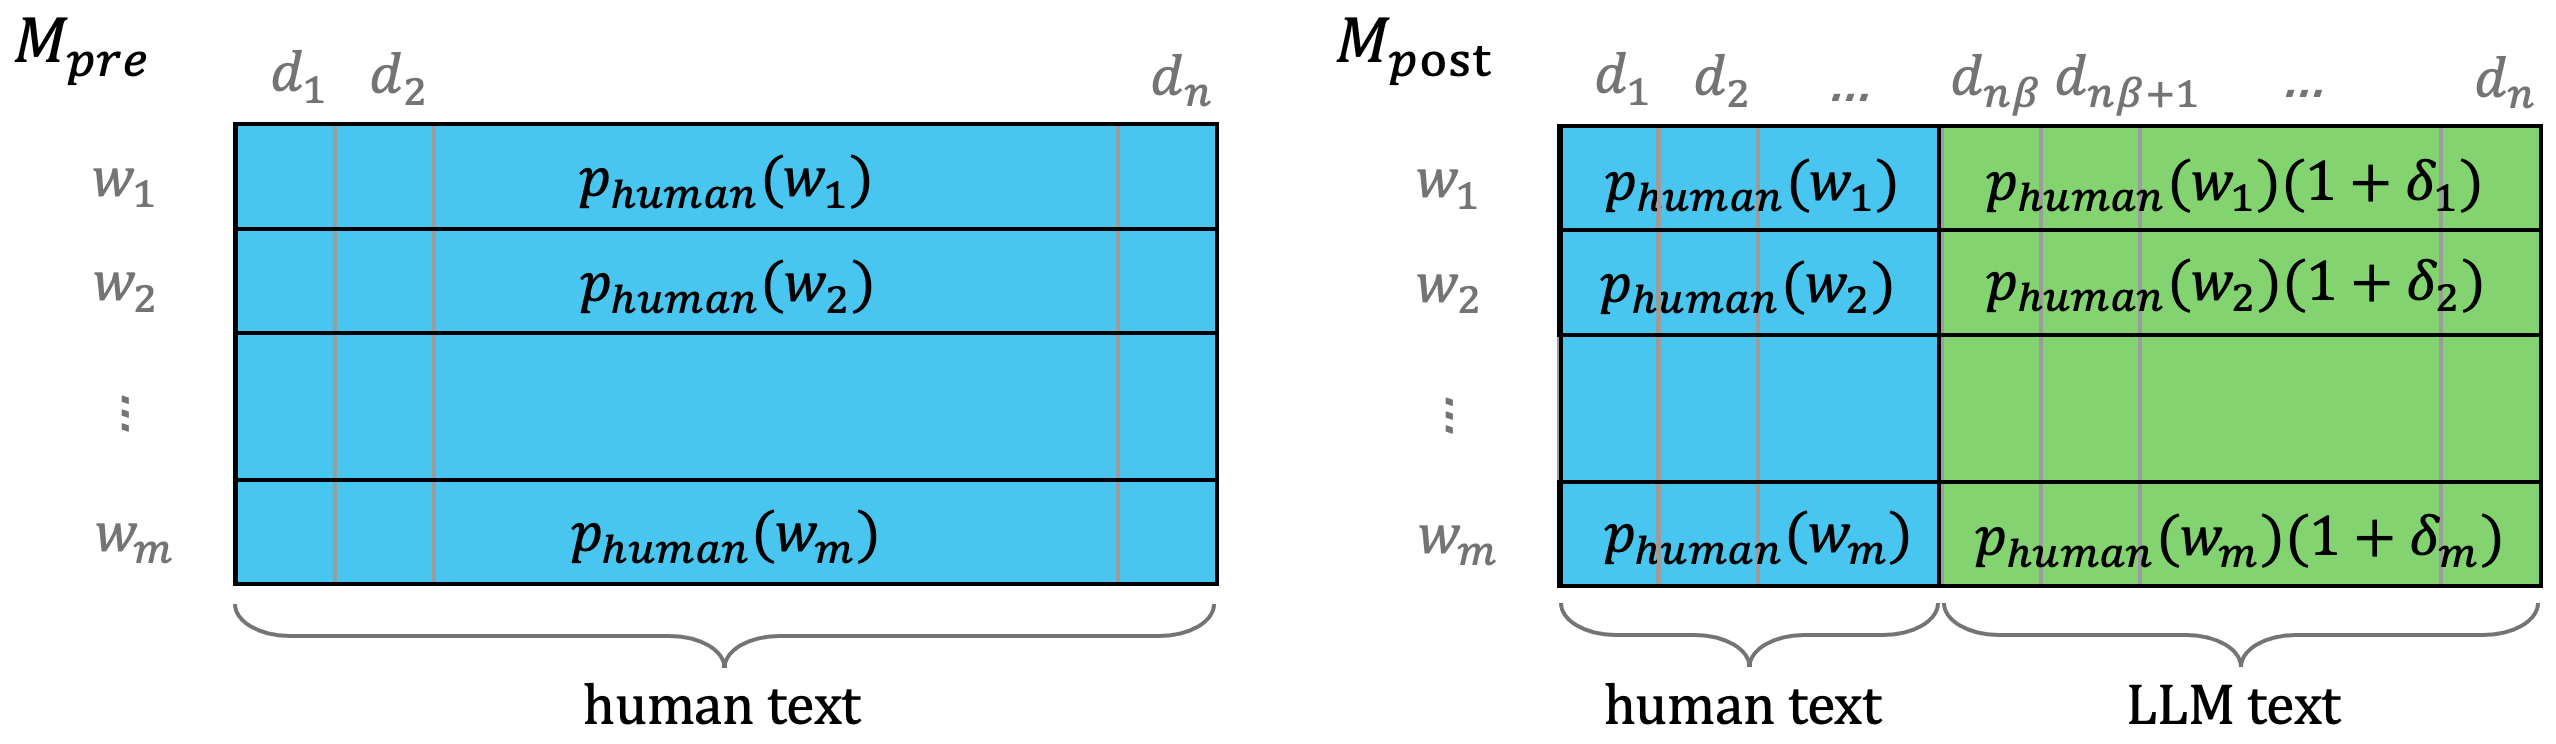
\includegraphics[width=0.9\linewidth]{../results/plots/misc/intuition_simulation_v2.png}
    \caption{Illustration of the sampling procedure for the creation of an artificial dataset to test the LLM use estimate $\hbet$ for varying levels of $\beta$}
    \label{fig:intution_simulation}
\end{figure}
To better gauge how well the procedure of finding the optimal excess word list to get the best possible lower bound works, we performed the same analysis on simulated data with known $\pl$ and $\ph$ and varying $\beta$.
We simulated data for 100,000 texts, approximating the number of papers per year in our sample.
In our simulation, there were 500 words, all of which were treated as excess words.
We created two matrices, $M_{pre}$ and $M_{post}$, each with dimensions (\emph{number of texts, number of words}), corresponding to data before and after the release of ChatGPT, respectively.
For $M_{pre}$, each word $w$ was randomly assigned a probability $\ph(w)$. 
The probabilities were sampled from a gamma distribution with shape parameter $2$ and scale parameter $0.02$.
Then, 100,000 binomial samples were drawn with $\ph(w)$ as probability of success for each word.
For $M_{post}$, a fraction of $\beta$ texts were selected as being LLM-generated.
As one of the assumptions posits that $\ph\le\pl$, the probabilities for words to occur in LLM-assisted text were sampled as $\pl(w)=\ph(w)(1+\delta)$, with $\delta \sim U(0.5,5)$.
In cases where $\ph(w)(1+\delta)>1$, $\delta$ was newly sampled until the resulting $\pl(w)$ was in the range $[0,1]$.
In the sampling process $100,000\cdot \beta$ binomial samples were drawn with probability $\pl(w)$, and $100,000\cdot (1-\beta)$ were drawn with probability $\ph(w)$.
\\
For the following analyses, the word frequencies in $M_{pre}$ was treated as analogous to $\hph$, and those in $M_{post}$ as the observed frequencies $q$.
The words in $M_{pre}$ were ordered by frequency, and excess lists were formed of words with frequencies lower than those of several different cutoffs. 
For each excess list corresponding to one of the cutoffs, the LLM-use estimates $\Delta$ and $\hbet$ were computed.
The only difference w.r.t. the procedure on the real data was during variance computation: $M_{pre}$, as opposed to $\hph$, is not the result of a regression, but, similar to $q$ the result of a binomial sampling procedure. 
Thus, the variance for frequencies based on $M_{pre}$ was computed as the variance of a binomial estimator, $Var(M_{pre}) = \frac{p(1-p)}{n}$ with $p$ the observed frequency and $n=(1-\beta)\cdot n_{texts}$.
As with the real data, we exclude cutoffs yielding frequencies $\ge0.999$ for $M_{pre}$, as well as estimates with error bars $\ge0.025$.


\subsection{Section length}
One of the goals of this project was to compare the estimated LLM-use of different sections of the paper with each other.
This might seem like an unfair comparison: When using word occurrence as LLM-marker, longer texts are at an advantage - there is simply more space for words to appear in.
[Figure here shows the different section lengths]
For example, if an LLM produced some word once every 500 words on average, it would appear in the majority of 1000-word sections, but only in about half of 250-word sections, despite all of them being written by an LLM.
Since the word counts are binary, there is no correction for section length in the estimate.
This is a further argument for using section specific word lists instead of single words.
The longer the word list, and the higher their aggregated frequency, the less likely it is for an LLM-generated text, however short, to not contain at least one of them.
However, when authors use LLMs, it is also likely that they focus their usage on specific paragraphs that they, e.g., wish to rephrase.
A longer section contains more paragraphs that might warrant re-working.
One way to address this issue is to slightly shift the question from \emph{How high is LLM-use in this section?} to \emph{How high is LLM-use in a random paragraph of this section?}
% By focusing on paragraphs instead of full sections, the section length can be controlled for. 
This was implemented by cropping each section sample to a length of 255 words, which corresponds to the median length of the abstracts.
The cropped part was placed randomly within the section by sampling a starting position ranging between the first and 255th-last words in the text.
Note that the LLM-use estimate based on the cropped sections can't be used to determine the full fraction of papers that were written with some LLM participation.
Since we are interested in identifying not only those papers that are wholly written by an LLM, using only one paragraph per section will underestimate the number of papers written with the help of LLMs, because this paragraph might not include the parts of the paper where LLMs were used. 
However, by comparing the results from the full and cropped sections, we can check whether LLMs are used universally across the entire paper or whether their use is concentrated on some paragraphs.



\subsection{Subgroup analysis}
%comment: add plot with number of paper per country (barplot for ind country counts, say 2017 to 2025, pie chart with entries "english-speaking", "non-english speaking", "unknown country")
Another point of interest is how LLM-use differs across subsets of the data.
It is, for instance, plausible to assume that majority English-speaking countries will show different usage patterns than countries where English is learned as a second language.
Likewise, there might be differences between academic disciplines, with some being quicker to adopt a new technology.
Previous studies typically reported higher usage estimates for research areas related to computer science.
To compare these categories, we repeated the experiments on different subsets of papers.
\\\\
\emph{Countries}
\\
The most salient criterion to compare countries with each other when it comes to LLM-use is their majority native language.
Since English is the de facto lingua franca of academia, one of the key capabilities of LLMs is their ability to translate or proofread text from authors uncertain of their English proficiency.
As this use-case is irrelevant for native English speakers, it stands to reason that LLM-usage would be smaller for English-speaking countries.
\\
To categorize countries into English and non-English speaking, we used the \emph{Three circles of English model}\cite{kachru1985standards}, which sorts the United States, the United Kingdom and Ireland, Australia and New Zealand, South Africa, and the majority of Canada into the ``inner circle'', where English is the native language of the majority of inhabitants and primarily used in their day-to-day lives.
All other countries were classified as non-English speaking. 
Additionally to comparing English to non-English speaking countries, we also analyzed the LLM-use of individual countries.
We selected the 18 countries with highest paper counts in the years 2017 to 2025.
The full list of countries and their respective paper counts can be found in the Appendix.
\\
We originally planned to use the excess word lists that are optimal for each section with regards to the full dataset. 
However, this lead to observations of $q=1.0$ for several years and countries (pre- and post-release of ChatGPT).
Due to time constraints, it was unfeasible to search for the optimal list for every country and section.
As a heuristic to approximate the search process, the list corresponding to the next-lower cutoff was selected.
For example, for the abstract, the optimal cutoff was $0.1$, so we selected the list corresponding to a cutoff value of $0.07$, which was the value directly preceding $0.1$.
By lowering the cutoff, we reduce the number of words in the excess word list and can thus regulate the observed frequencies.
This ``suboptimal'' cutoff also lead to problematic observations, because in many cases, $q$ was within the regression error of $\hph$, which is not ideal for any metric depending on the difference between the two.
To adjust, we moved the cutoff value one position further down, e.g. by going from $0.1$ to $0.05$ instead of $0.7$ for the abstract.
\\\\
\emph{Research disciplines}
\\
%comment same plot as for countries, maybe put in appendix? or do table instead of plot?
Papers were sorted into different research areas based on the titles of journals in which they were published in a procedure based on \cite{gonzalez2024landscape}.
The research areas are subfields of the biomedical domain, for example radiology or nursing, that were specified in \cite{gonzalez2024landscape}.
The full list of categories can be found in the Appendix.
Journals were sorted into a category via keyword search with the category titles, and were assinged no label in case of no match.
This is a relatively crude but simple approach that ignores many potential matches, e.g., the (hypothetical) \emph{Journal of Neurology} would be assigned the label ``neurology'', while the \emph{Neurological Journal} would not. 
The number of matches could be improved by using fizzy matching or manually annotating 
In assigning labels, the keyword appearing latest in the title was given precedence. 
For example, the \emph{Journal of Cancer Biochemistry} would be sorted into the ``biochemistry'' category, while \emph{The Biochemistry of Cancer} would be assigned the label ``cancer''.
This procedure resulted in 23\% of papers being labeled.
Only labels with more than 5000 papers were selected for further analysis.
Using the optimal excess word lists to compute frequencies lead to similar problems as detailed above, which is why we also used the cutoff twice removed from the optimal one.


%\section{Results}\label{sec:results}
\subsection{Simulation}
%comment: these plots should ideally also include the sampling distribution (or put that in the methods?)
\begin{figure}[htbp]
    \centering
    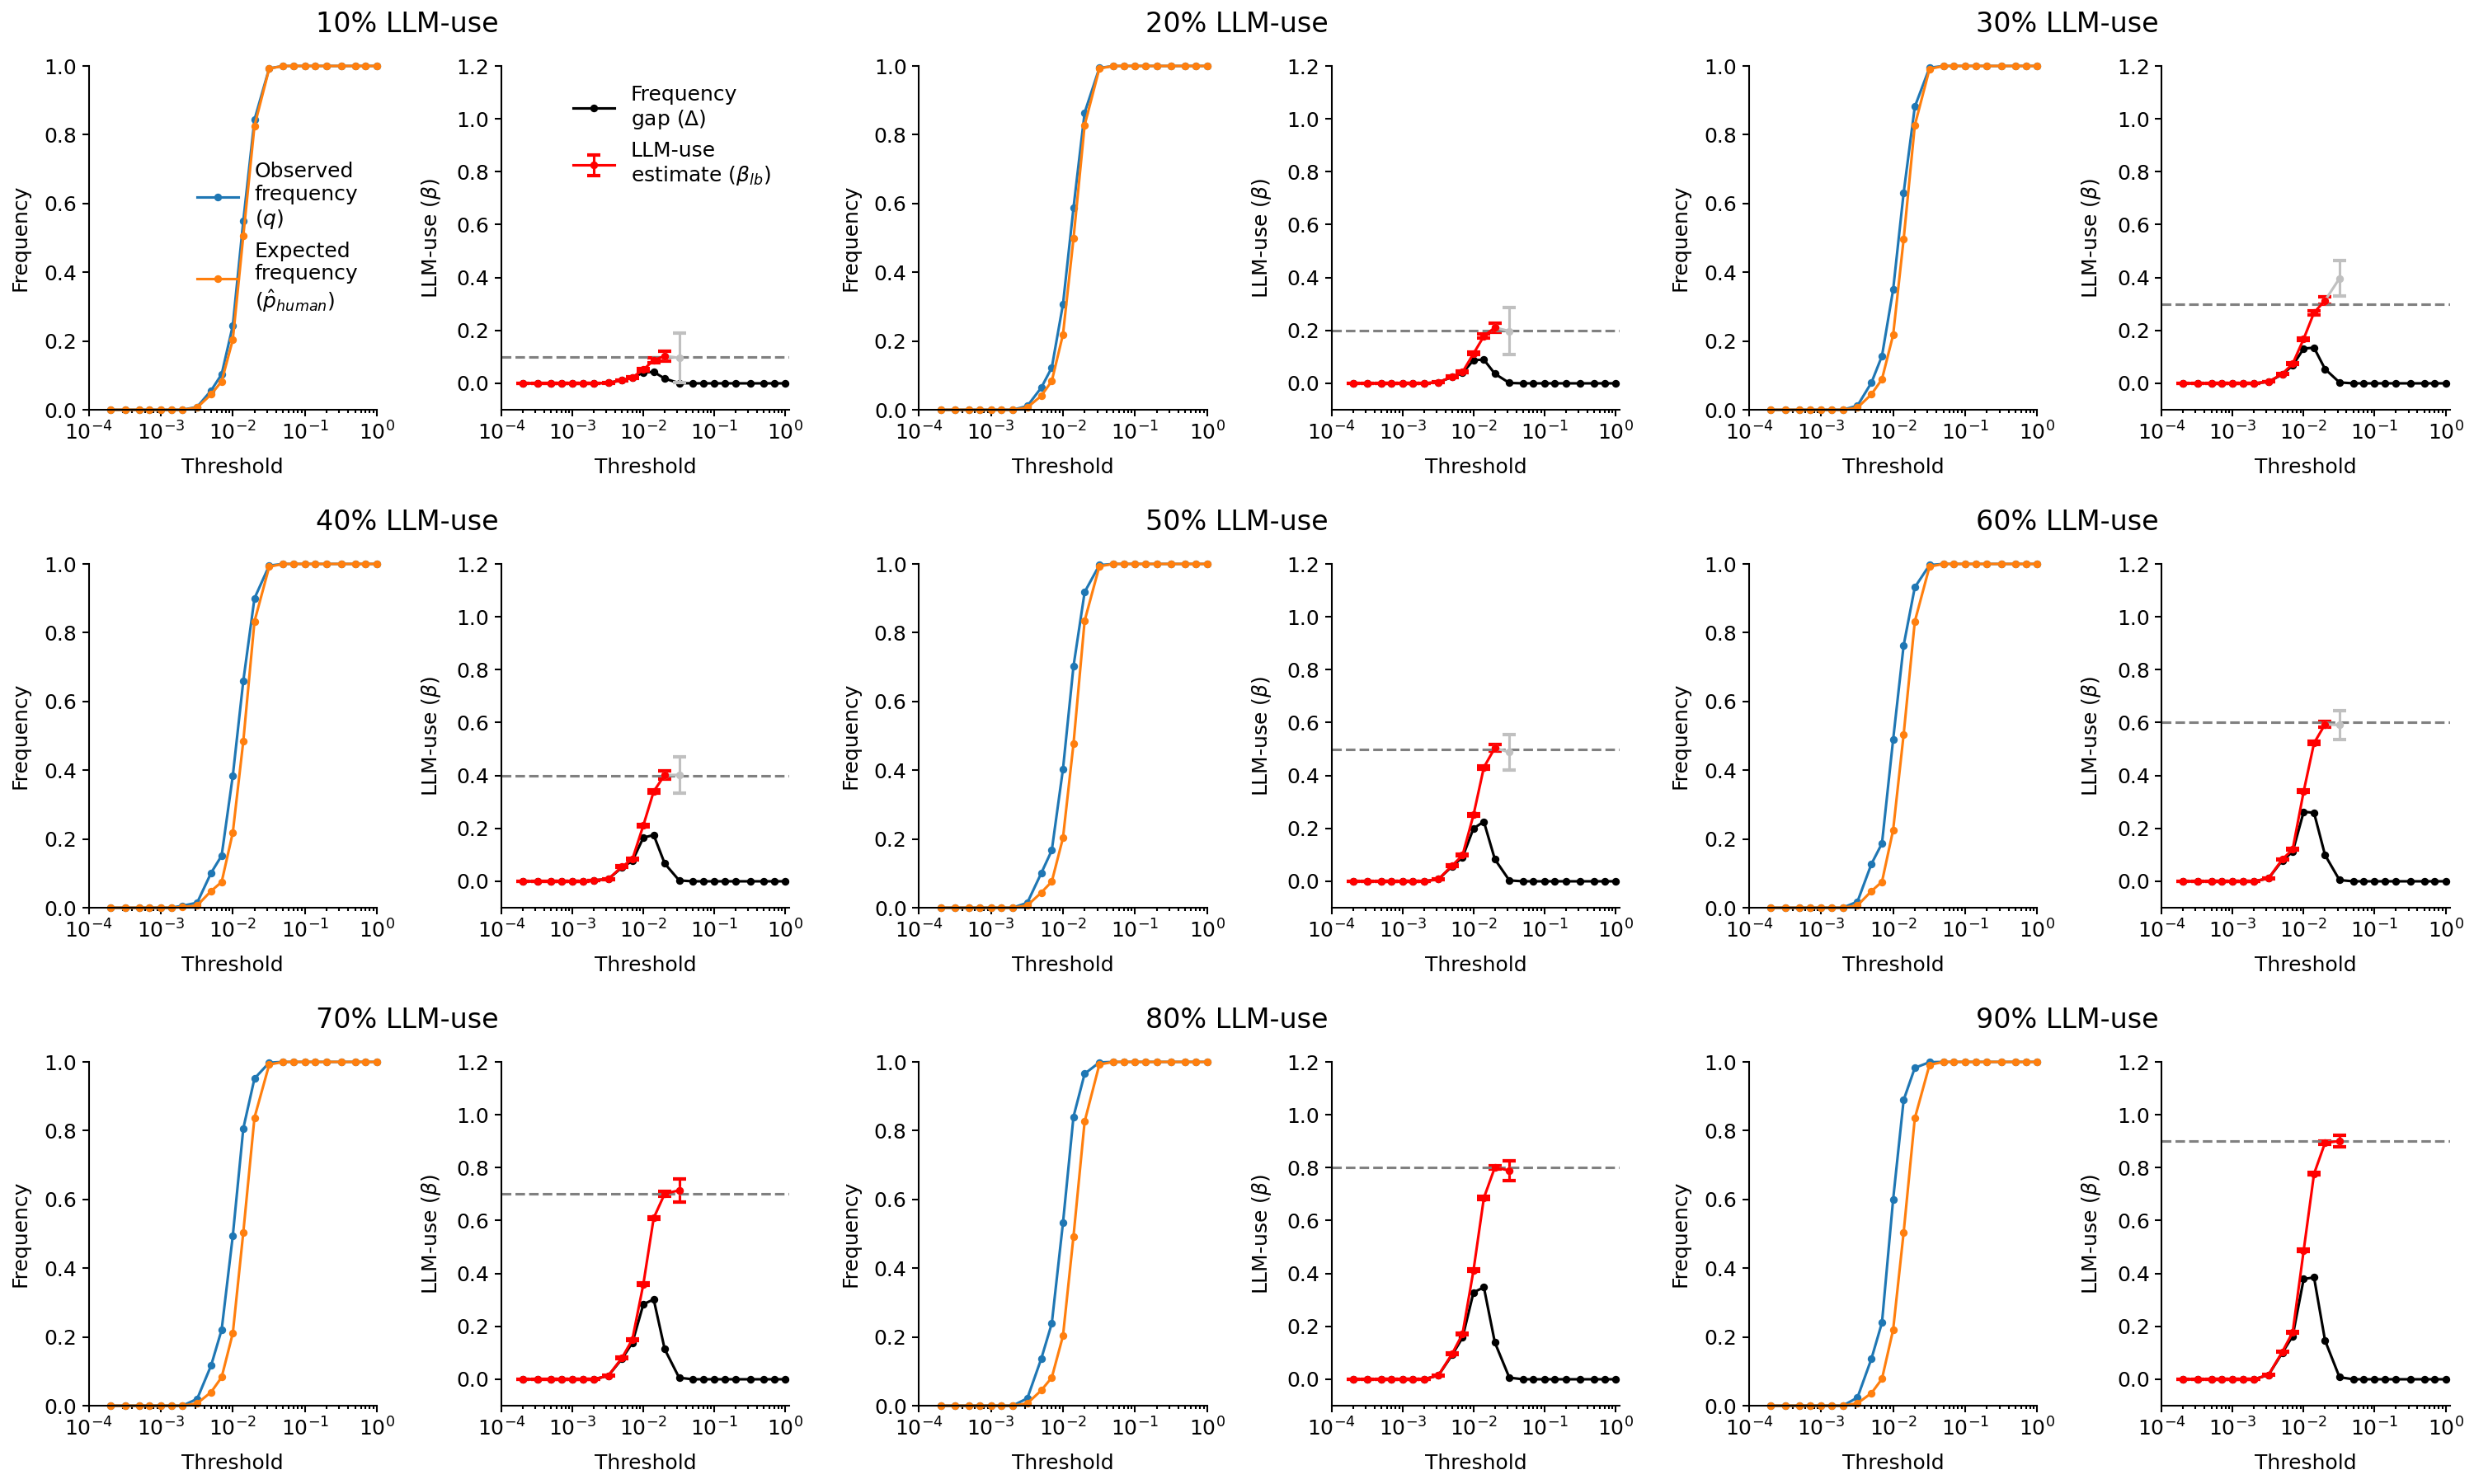
\includegraphics[width=\linewidth]{../results/plots/ground_truth_simulation/500_words.png}
    \caption{}
    \label{fig:simulation500}
\end{figure}
\begin{figure}[htbp]
    \centering
    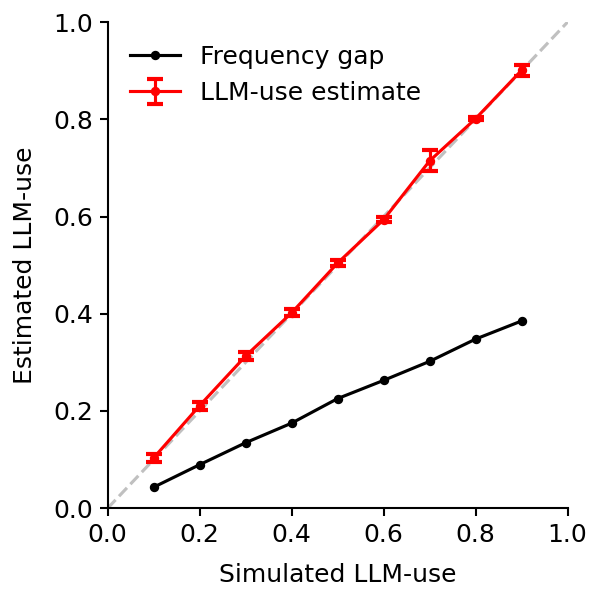
\includegraphics[width=0.5\linewidth]{../results/plots/ground_truth_simulation/500_words_overview.png}
    \caption{}
    \label{fig:simulation_overview}
\end{figure}

\subsection{Individual word estimates?}
%comment: might be interesting to include section comparison of individual words, need the plots for that
\subsection{Word list estimates}
\begin{figure}[htbp]
    \centering
    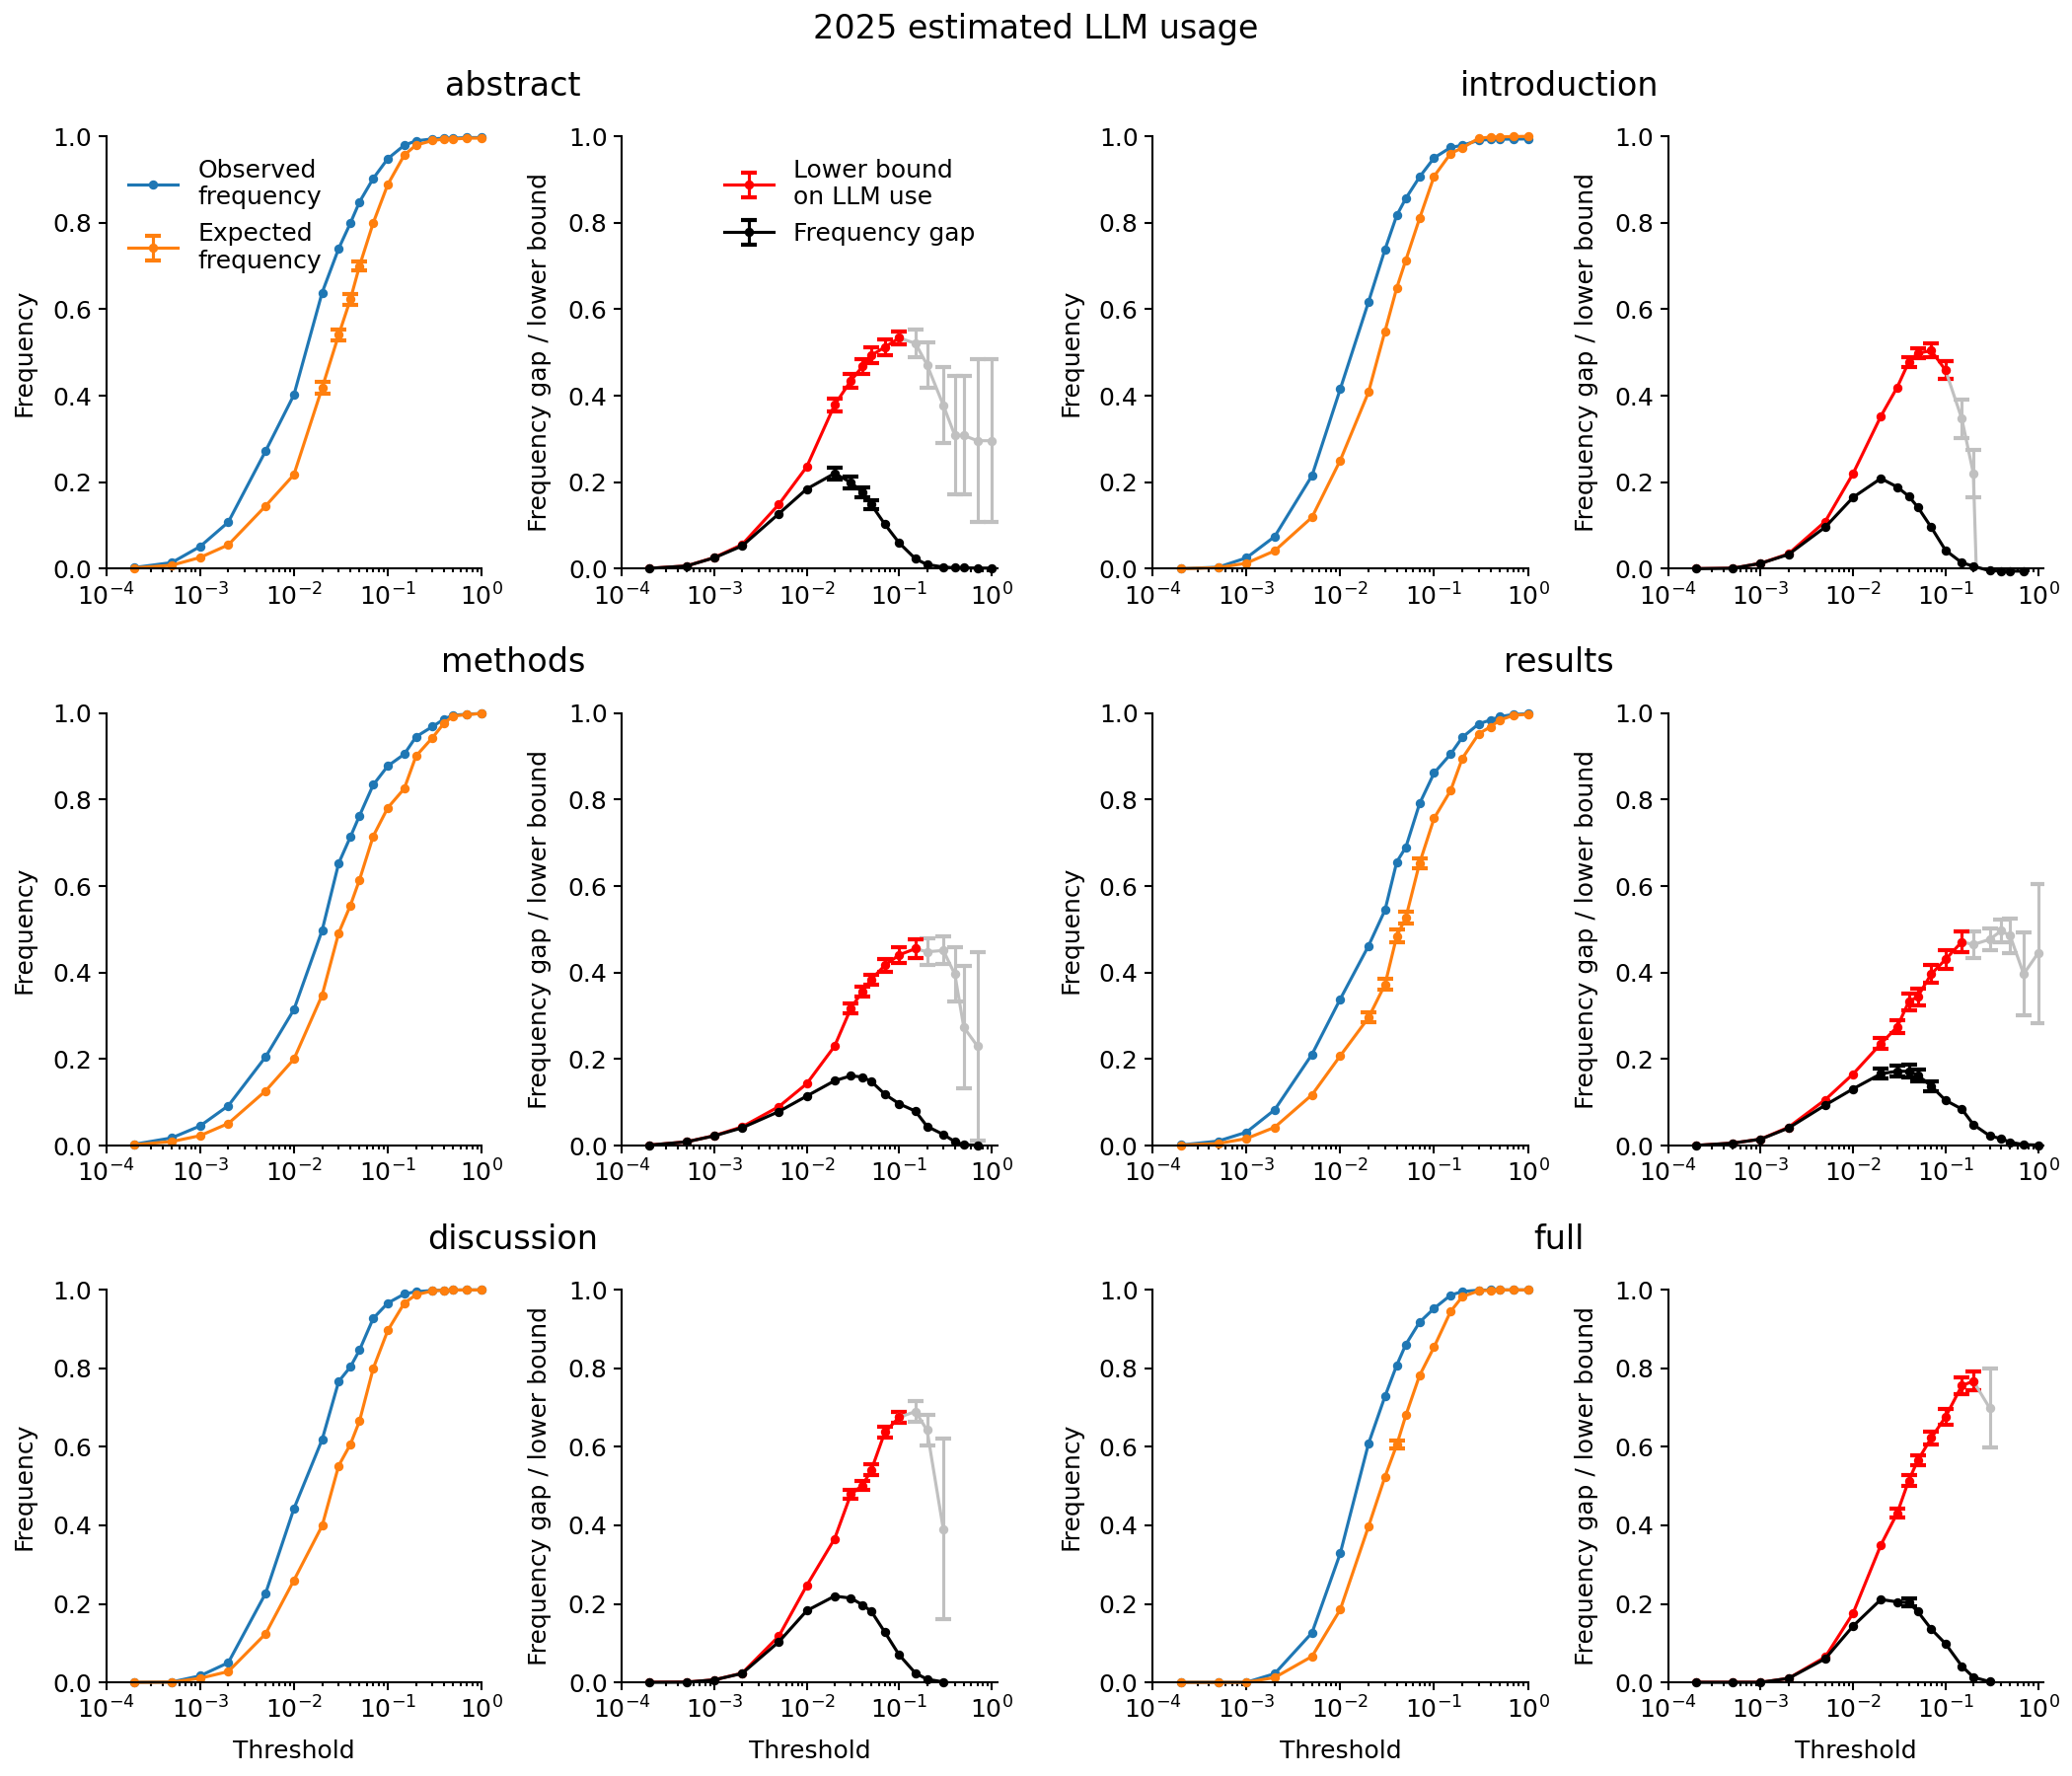
\includegraphics[width=\linewidth]{../results/plots/baseline_2026-01-23/research-article_aimrd_f/5y_2025_lower_bound_non_lemmatized_.png}
    \caption{}
    \label{fig:2025_optimization}
\end{figure}
\begin{figure}[htbp]
    \centering
    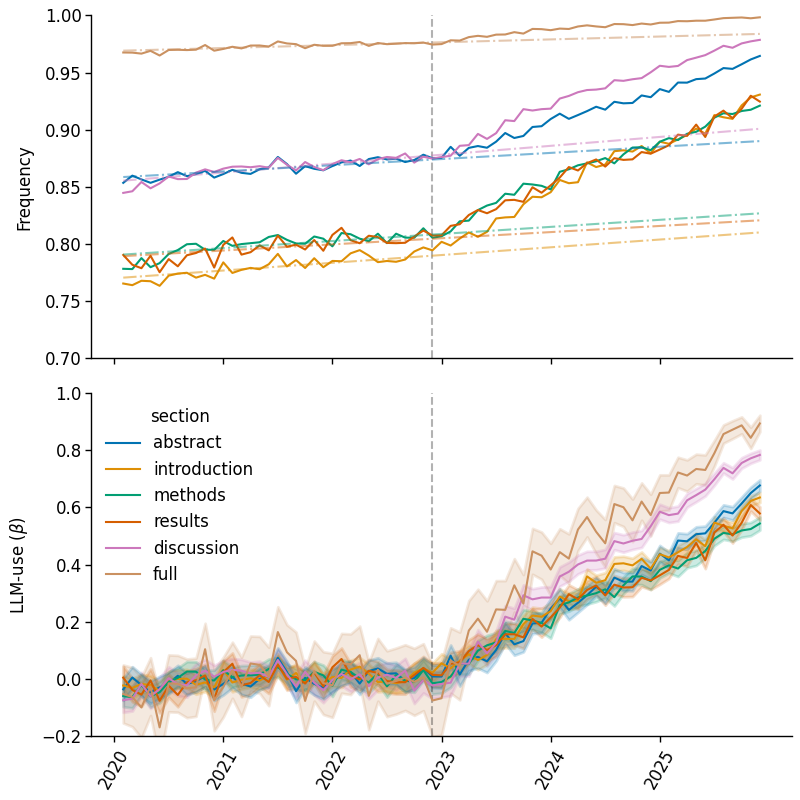
\includegraphics[width=\linewidth]{../results/plots/baseline_2026-01-23/research-article_aimrd_f/group_freqs_time.png}
    \caption{}
    \label{fig:monthly_est}
\end{figure}
\begin{figure}[htbp]
    \centering
    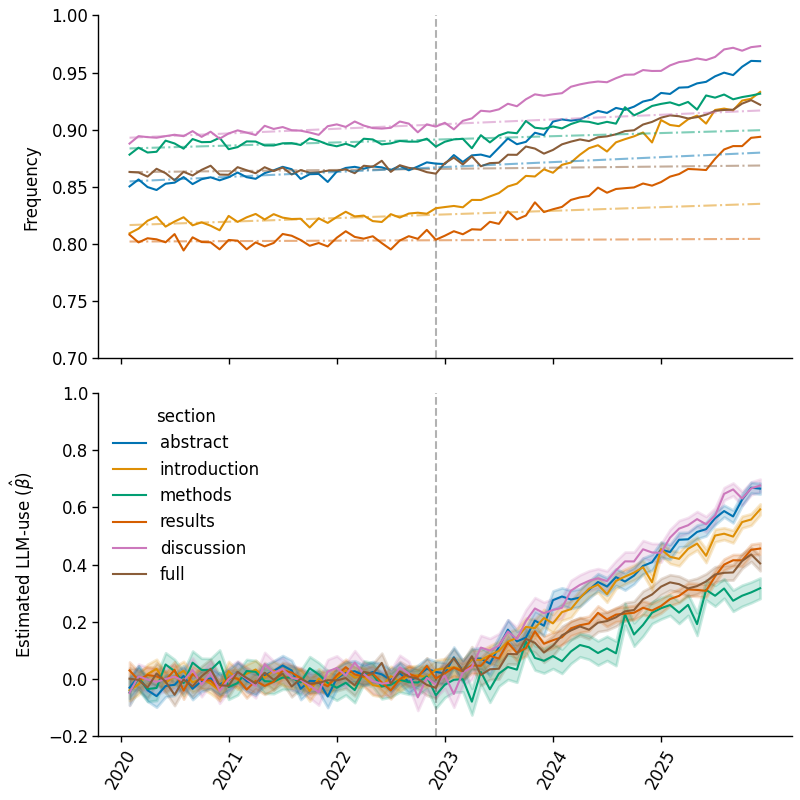
\includegraphics[width=\linewidth]{../results/plots/baseline_2026-01-23/research-article_aimrd_f_crop255/group_freqs_time.png}
    \caption{}
    \label{fig:monthly_est_crop255}
\end{figure}

\begin{figure}[htbp]
    \centering
    \begin{minipage}[t]{0.48\textwidth}
        \centering
        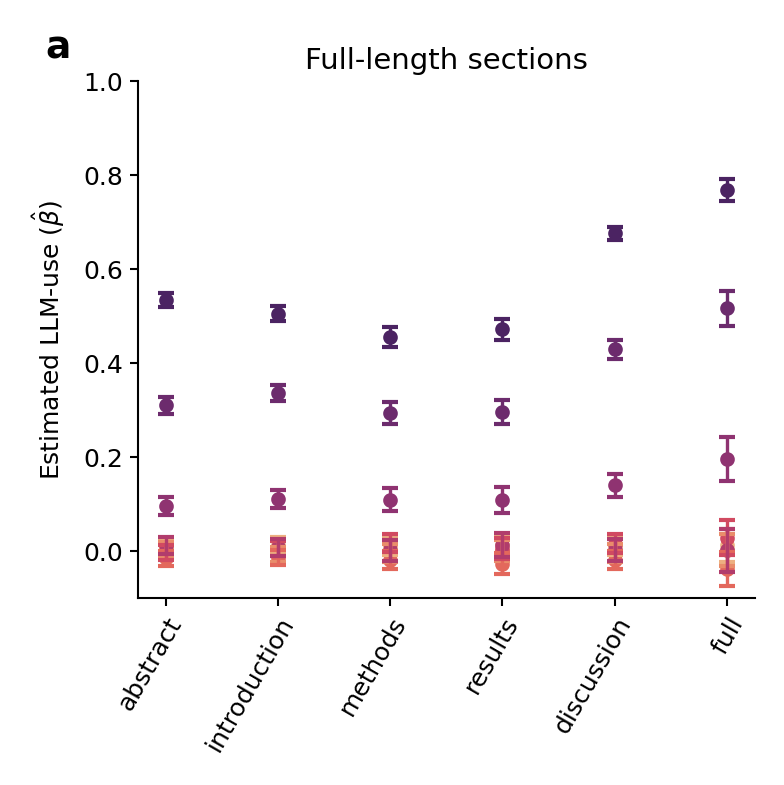
\includegraphics[width=\linewidth]{../results/plots/baseline_2026-01-23/research-article_aimrd_f/group_freqs_section_single_panel.png}
    \end{minipage}
    \hfill
    \begin{minipage}[t]{0.48\textwidth}
        \centering
        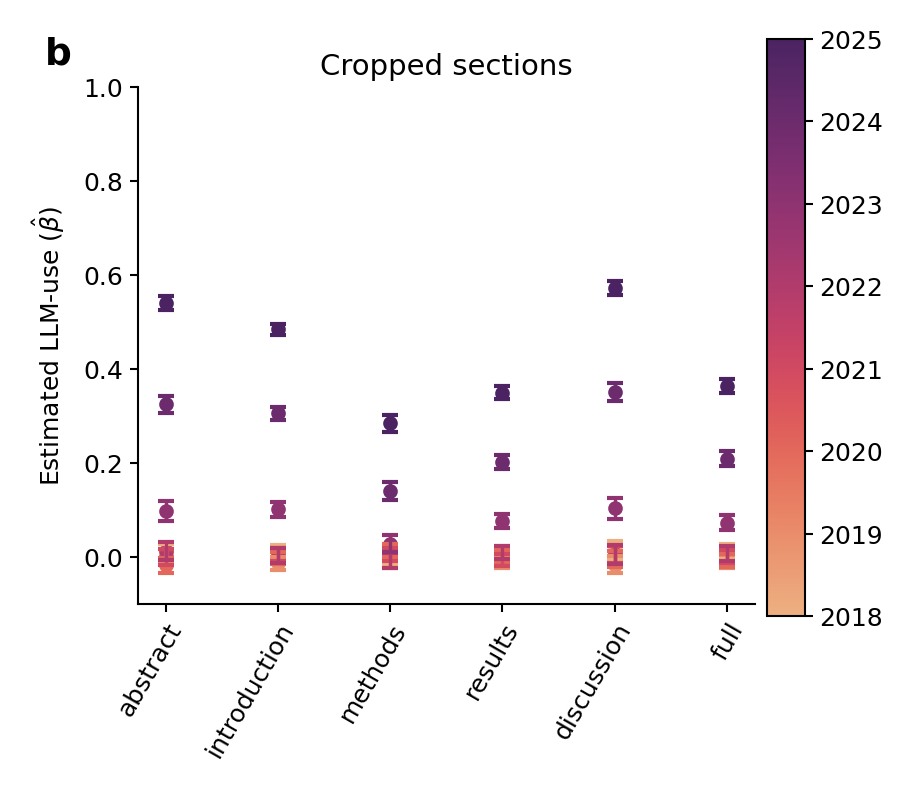
\includegraphics[width=\linewidth]{../results/plots/baseline_2026-01-23/research-article_aimrd_f_crop255/group_freqs_section_single_panel.png}
    \end{minipage}
    \caption{Shared caption describing both images}
    %comment: re-do this to only have one colorbar and title referring to full sections/cropped sections, also there should be no line connecting the dots 
    \label{fig:est_per_section}
\end{figure}
%\section{Discussion}\label{sec:discussion}

\subsection{The estimate $\hbet$ reliably predicts LLM-use}
The LLM-use estimate $\hbet$ introduced in this work is a lower bound on actual LLM use derived from observed and counter-factual word frequencies. 
It makes use of the observation that LLMs show a preference for a group of words identified by Kobak et al., which they call excess style words  \cite{Kobak2025}.
By tracking the excess word frequency in a corpus before the wide-spread availability of Chatbots, we can estimate the frequency expected for the following years without the influence of LLMs on the writing process, $\hph$. 
To accurately determine LLM-use $\beta$, we would also need access to the frequency in a corpus of LLM-generated or LLM-assisted text.
Because this is not possible (without creating a curated collection of LLM-text), we replace $\pl$ with 1 in the equation for $\beta$, arriving at the lower bound $\hbet$.
\\
While $\hbet$ is a lower bound, it moves closer to true $\beta$ if $\pl$ gets closer to 1.
This can be achieved by selecting a group of words with collective high frequency to base the estimates on, which we do by incrementally increasing the frequency cutoff determining which words are selected for the word list, and computing the estimate for each list.
The danger of this approach is that if $\pl$ is very close to 1, so is $\hph$, resulting in both the numerator and denominator of the equation for $\hbet$ going towards 0, which causes strong fluctuation in the estimates, and yields division by zero errors in the worst case.
To avoid this, we constrain the search for the optimal cutoff such that $\hph$ must be below $0.999$ and the standard deviation error must be no bigger than $0.025$.
The simulation experiment tested the validity of this procedure.
We were able to identify the correct underlying proportion of LLM-assisted text for every ground-truth value tested.
This demonstrates the improvement toward the previous lower bound, $Delta$, which systematically underestimated LLM-use. 
Notably, some cutoff values that would have lead to an overestimation were excluded from the analysis by the constraints, indicating their importance.
The choice of $0.025$ as the maximum standard deviation is arbitrary, but has a potentially strong effect on the estimates.
For example, the estimate for LLM-use in the results section for 2025 would have been somewhat higher, if a higher threshold would have been chosen (see Figure \ref{fig:2025_optimization}).
Likewise, the estimates for the full paper reach their peak in the constrained regions for 2023 and 2024 (see Figures \ref{fig:2023_optimization} and \ref{fig:2023_optimization} in the Appendix).
On the other hand, as shown in Figure \ref{fig:simulation500} in the $30\%$ panel, overestimation of the true LLM-use is possible.
This should not happen in a lower bound metric, however, $\hbet$ is subject to some uncertainty, because it is computed with information that was empirically observed (in the case of $q$) or estimated with linear regression ($\hph$).
%comment: maybe depletion is predicted by q=1? but then all estimates would be 1, and this is not true for all depleted metrics. it can't be ph > q, cause then the estimate would be below 0, for the same reason it cant be ph>pllm, cause that implies ph > q, so what could it be?
The constraints on the standard deviation serve to keep this uncertainty in check, so the relatively conservative value of $0.025$ was chosen.
\\
Another peculiarity of the optimization curves is that they are almost always bell-shaped, and it is not clear why that should be the case.
Intuitively, the LLM-use estimates should increase with the number of words in the word list, as more words equal more LLM-markers to potentially be detected.
The bell shape could be an artifact of the estimates' increasing uncertainty.
To get a clearer image of this, we would need to adapt the frequency sampling for the simulations.
In the current version, the binomial probabilities that the simulation matrices are sampled from are distributed by a simple heuristic, such that the bulk of them have relatively low frequency with some outliers in the high-frequency region.
%comment: get a similar plot for distribution of real frequencies
However, in the optimization procedure, the observed and expected frequencies saturate to 1 much quicker than their empirical counterparts, such that they reach the constrained region of $\hph > 0.999$ earlier.
A sampling procedure yielding a distribution nearer to the empirically observed ones could improve understanding of the metric when both $q$ and $\hph$ are moving towards 1.

\subsection{LLM-use is continually on the rise across sections, countries and academic disciplines}
We observe a steady increase in LLM-use over the last three years, going up to $77\%$ in the main body of papers from 2025, and $89\%$ in the main body of papers from December 2025, the last time span considered here.
Using LLMs to edit or write certain parts of a paper has become commonplace in academia.
As shown in Figure \ref{fig:monthly_est}, this trend starts almost immediately after the release of ChatGPT, indicating a fast adoption of the new technology by scientists.
The rate of adoption also seems to follow a linear trend, which suggests that LLM-use is likely to continue growing in the future.
The pattern of continually increasing LLM-use also holds for the investigated subsets of PMC.
In all of the selected countries, language regions and academic disciplines, the highest LLM-use is observed in 2025, although the adoption is not as linear as in the combined set.
For example, the USA, the Netherlands and Brazil only show significant signs of LLM-use starting in 2024 (see Figure \ref{fig:countries_all}).

\subsection{LLMs are used more by NNES}
In line with our expectations, LLMs are used nearly twice as much in majority NNES countries as opposed to NES countries.
This trend has been reported in many other studies and surveys \cite{}. %comment: get citations.
An interesting country in this context is Canada, where people are NES only in some regions.
Accordingly, its LLM-usage is grouped between the NES and NNES countries.
The only outlier with regard to LLM-use is France, which has the third-to-lowest usage estimate in 2025 and the second-to-lowest in 2024 out of all investigated countries.
%how to explain? french people don't like technology?
Interestingly, the increasing use of LLMs seems to lead to the assimilation of the word frequencies in NNES and NES text. 
The frequencies of the selected word list was significantly higher in NES countries before the introduction of ChatGPT, but as of 2025, this gap is closed.
Because the word list only contains style words, this means that LLMs don't only help to avoid mistakes, but help users to adapt to a NES writing style, acting as ``linguistic equalizer'' \cite{Lin2025_NES,Prakash2025}.

\subsection{LLM-use estimates vary between (some) sections}
%comment: where to put this?: uncertainty and fluctuation is much bigger for full section, also exceeding the constraints, because the estimated were computed with the optimal word list for 2025, which might not be optimal for the previous years
%comment: need section length plot!

The LLM-use estimates of different sections were more similar than expected, with at most seven percentage-points differentiating the abstract, introduction, methods and results, with the abstract yielding the highest estimate among the four in 2025, but being second to the introduction in 2024.
The discussion is clearly the section with highest LLM-use, with estimates up to fifteen percentage-points higher than the abstract.
Because the estimates for the main body of the paper includes all sections except the abstract, and there are individual sections with higher estimated LLM-use than the abstract, the main body estimates are necessarily the highest, because they are an upper bound for the other sections.
This is because we calculate word occurrence and not word frequency within a text as the basis for our frequency measure, so if a word appears in any one section, it also appears in the full text.
\\
The big gap between estimates for individual sections to those of the full paper indicate that it's not the case that LLMs are always used uniformly across the paper, such that a high LLM-use estimate in one section doesn't necessarily predict high LLM-use in other sections.
Instead, many papers seem to have been written with relatively selective use of LLMs, where only certain sections were altered.
On the other hand, the LLM-use estimates of the discussion are not much smaller than those of the full paper, indicating that if there were LLM-generated passages somewhere in a paper, it would most likely be in the discussion.
Also, even with the gap between full paper estimate and individual sections estimates present, it is not nearly big enough to indicate that only one section per paper had been edited (this also would be a highly unlikely scenario).
All in all, this suggests the most common use of LLMs is to edit certain paragraphs of the paper, that might or might not be in the same section, with the discussion having the highest likelihood of being edited.
To further investigate this, sections could be grouped in the counting process, to indicate whether a marker word occurs in both sections.
\\
These observations alleviate a potential concern of our method, namely that the excess words identified in 2024 PubMed abstracts would be vocabulary tailored specifically to abstracts, and thus would only reliably pick up on LLM-use within abstracts.
To guard against this, the excess word list was sorted according to the frequencies within each section during optimization, and each section was optimized separately (although, as previously discussed, the individual optimization means that some sections might be impacted more by the constraints than others).
It could still be that LLM-use in all sections except the abstract is underestimated, but as the discussion and, for some intervals, the introduction yield higher estimates than the abstract, it is at least not the case that our method favors the abstract to the point of always attributing highest LLM-use to it.
In fact, when looking at the results for different countries and disciplines, the main body of the text almost always yields higher estimates than the abstract, the only exceptions being Australia and France, which, as discussed previously, is an outlier in other regards as well.
\\
Of course, the abstract is by far the shortest of the investigated sections, and is much shorter when compared to the main body of the text.
There are many more paragraphs that could have been rewritten with the help of an LLM, many more words that could have been replaced with marker words while editing.
To normalize for section length and investigate how likely it is for any paragraph within a section to have been altered with the help of LLMs, we repeated the experiments with cropped versions of the sections.
%comment: it's not really normalization
There is barely any difference between the LLM-use estimates of the full and cropped abstracts, which is to be expected as any random crop of 255 words (the median length of the abstracts) will contain most or all of the abstract in question.
The difference between full and cropped introductions is also very small (two percentage points, which is within one of the error margins), indicating that if an LLM was used to edit the introduction, changes were made to the entire section as opposed to single paragraphs.
For results and discussion, the changes from full to cropped are somewhat larger, with twelve and eleven percentage points respectively.
This indicates that while LLM-use is still relatively evenly spread among different paragraphs in these sections, there appears to be some clustering of markers.
The biggest difference between the full and cropped versions is measured in the methods section, showing that LLM-use is most clustered here.
However, it could also be that there are more linguistic restrictions in certain parts of the methods section, which don't allow the replacement of words with LLM markers. 
For example, reporting the technical details of some experimental setup usually follows a typical structure that doesn't leave space for the style words we use to detect LLM-use.
This means that LLMs might be used universally in all paragraphs of the methods section, but only change the vocabulary in some.
\\
Overall, a single paragraph sampled from the discussion or abstract has the highest likelihood of having been edited with an LLM, followed by the introduction, results and full text, with methods coming last.

\subsection{Comparison to other estimation methods}
 - advantage of not relying on ground-truth text: not vulnerable to different results stemming from different prompting strategies (Dou enhancing robustness 2024) (disadvantage is only lower bound, but as was shown, we get reasonably close to the actual value)
- going beyond word frequency: other linguistic markers as LLM indicators (perplexity, sentiment, part-of-speech, vocab size and density) e.g. \cite{Guo2023}, Bao Tong 2025, or intrinsic text embedding dimensionality \cite{Tulchinskii2023}, or repeated higher-order n-grams \cite{Gall2021} (although this is for GPT2 and might be no longer true)


\subsection{Limitations}
Some concerns about our method have already been discussed in previous sections of the discussion.
The LLM-use estimate $\hbet$ behaves unreliably in the limit regions where $q$ and $\hph$ go towards one, which is critical because this is also the area in which it is most likely that $\pl=1$, thus giving the most reliable results.
The constraints introduced to avoid unreliable estimates in the limits may lead to a disparity between sections, as the sections are optimized individually, so for some, the optimal estimate might lie in the constrained region. 
Because suboptimal estimates are to be preferred to unreliable ones, the constraints were kept at a relatively conservative level. 
Another limitation is our inability to perform excess word search for each section in our dataset, being limited to using the list established in prior research by Kobak et al. \cite{Kobak2025}.
Since the excess words are domain-independent, %comment: are they?
they should have equal validity for each section and the optimization procedure is still section-specific.
\\
A more severe limitation is that our estimates are, by design, dependent on changes in word frequency between human and LLM-generated text.
By using only marker words, we are unable to detect LLM-generated text that, by using a distinct prompting strategy \cite{Geng2025} or by chance, doesn't contain any excess words.
This is somewhat mitigated by the length of the excess word list, it is much harder to purposefully or accidentally exclude over 300 words, compared to the small selection used by other authors \cite{Gray2025, Gray2026, Kousha2025}.
However, the main concern doesn't focus on $\pl$, but on $\ph$.
Our estimate hinges on the central assumption that $\hph$ is a faithful estimate of $\ph$. 
For the months immediately following the release of ChatGPT, this is a reasonable assumption, as $\ph$ follows a linear trend that can be modelled with linear regression.
As we move away from this date, confidence in $\hph$ decreases, because the environment that academic text is produced in fundamentally changes with the introduction of LLMs.
The more papers are written with the help of LLMs, the more people will become familiar with their writing style, and might start consciously or subconsciously copying it.
They might also use LLMs for other tasks, thereby learning the types of suggestions LLMs typically make and adapting those into their own writing process, without repeated input from the LLM.
LLMs have already been shown to influence human speech.
Yakura et al. \cite{Yakura2025} investigated changes in word frequency in academic talks on YouTube and conversational podcast episodes and found increasing use of ``delve'' after November 2022 in both datasets.
While both of these media forms rely on scripted content to some extent (the podcasts showing hints of LLM-use were educational and situated in the realms of science and technology, business and education, rather than casual conversations), the podcasts will likely also contain segments of spontaneous speech. 
Even though there is some evidence for the influence of LLMs on human speech, it is unclear how quick and how pervasive this adaption to an LLM-style of writing will take place.
Previously uncommon words like ``delve'' are very salient signals because their sudden appearance after relative obscurity generates more attention \cite{Geng2025}.
This also makes them more likely to be copied, especially for NNES who might not have known the word previously and added it to their vocabulary only after coming across it in LLM-generated text.
On the other hand, changes in the frequency of common words are much harder to pick up on.
When reading a text, it doesn't really make a difference to the reader if the word ``these'' appears two or three times.
Changes in high-frequency words only really register when looking at a large corpus of text, whereas humans interacting with LLMs or reading LLM-assisted papers only have access to a small selection.
This makes it less likely for them to be copied directly.
Geng and Trotta \cite{Geng2025} therefore argue for focussing on high-frequency words when trying to detect LLM-generated text, although with the rising influence of LLMs, it is unclear for how long this advantage will hold.
High-frequency words might for example be part of certain phrases that LLMs prefer, which could be copied by users.
To investigate this, the analysis could be widened to include higher-order n-grams.


\subsection{Impact}
impact / normative evaluation: overcoming language barriers, science papers rely on the data that is being reported, writing style is not immediately important. However, writing is a technology to sharpen our thinking. It takes effort to write something down. In deciding how exactly to phrase something, we are forced to think very precisely about our work, a level of scrutiny which makes it more likely that leaps of logic will be addressed that would have been brushed by when only engaging with LLM outputs



%\printbibliography

%\appendix
%\section{Survey results}
In all surveys, we focused on use cases that could have an influence on the formulation if final paper, such as editing or summarizing of other papers, instead of use cases in other academic undertakings, such as writing code, or very early in the writing process, like brainstorming or writing an outline.
Grammar checks were also excluded as a relevant use case, because while this is a very popular task for LLMs, this should have a minor influence on phrasing.
If use cases were not part of the survey, we took the general proportion of researchers reporting LLM use in at least some part of their research. 
an important factor in evaluating the results is the organization doing the survey.
Researchers might be hesitant to admit LLM use in a survey done by an important academic publisher despite anonymity, especially if this publisher is known to be anti-LLM, such as Nature

\begin{sidewaystable}
\centering
\begin{tabular}{lrlllrc}
\toprule
\makecell[c]{survey\\period} & \makecell[c]{sample\\size} & \makecell[c]{sample\\specification} & \makecell[c]{question} & \makecell[c]{category} & \makecell[c]{usage} & \makecell[c]{source}\\
\midrule

\multirow{2}{*}{\makecell[l]{04/2023--\\05/2023}}
& \multirow{2}{*}{456} 
& \multirow{2}{*}{urologists} 
& Do you use ChatGPT/LLMs in your academic practice? 
& general & 48\% 
& \multirow{2}{*}{\cite{Eppler2024}}\\
&&& summarizing text & writing & 27\% &\\

\midrule

\multirow{2}{*}{\makecell[l]{06/2023--\\07/2023}} 
& \multirow{2}{*}{3,838} 
& \multirow{2}{*}{postdocs} 
& Do you use AI chatbots, such as ChatGPT, in your work? 
& general & 31\% 
& \multirow{2}{*}{\cite{Nordling2023}}\\
&&& \makecell[l]{What do you use AI chatbots for? Refining text} 
& editing & 20\% &\\

\midrule

\makecell[l]{?--\\09/2023} 
& 1,659 
& \makecell[l]{researchers who\\had published\\in Q4 2022} 
& \makecell[l]{What do you use generative AI tools (e.g., ChatGPT, \\LLMs) for? To help write research manuscripts} 
& writing & 21\% 
& \cite{VanNoorden2023}\\

\midrule

\multirow{5}{*}{\makecell[l]{11/2023--\\04/2024}} 
& \multirow{5}{*}{816} 
& \multirow{5}{*}{\makecell[l]{researchers\\(Semantic\\Scholar)}} 
& Fix grammar or rephrase 
& editing & 50\% 
& \multirow{5}{*}{\cite{Liao2024}}\\
&&& Rewrite for another style & writing & 24\% &\\
&&& Shorten or summarize & writing & 23\% &\\
&&& Draft paragraphs from ideas & writing & 21\% &\\
&&& Direct writing (overall) & writing & 43\% &\\

\midrule

\makecell[l]{12/2023--\\02/2024} 
& 2,284 
& \makecell[l]{clinicians \&\\researchers} 
& \makecell[l]{Have you used an AI product or AI feature\\for a specific work-related purpose?} 
& general & 37\% 
& \cite{Elsevier2024}\\

\midrule

\multirow{3}{*}{\makecell[l]{01/2024--\\03/2024}}
& \multirow{3}{*}{2,021} 
& \multirow{3}{*}{\makecell[l]{researchers\\(Scopus)}} 
& \makecell[l]{Why use ChatGPT/AI tools:\\Synthesizing drafts to academic text} 
& \makecell[l]{\\writing} 
& \makecell[r]{\\16\%} 
& \multirow{3}{*}{\cite{Mohammadi2026}}\\
&&& Proofreading drafts & editing & 17\% &\\
&&& Translating text & writing & 18\% &\\

\midrule

\multirow{2}{*}{\makecell[l]{03/2024--\\04/2024}} 
& \multirow{2}{*}{1,043} 
& \multirow{2}{*}{researchers} 
& Help with translation & writing
& 40\% 
& \multirow{2}{*}{\cite{Wiley2025}}\\
&&& proofreading and editing scholarly papers & editing & 38\% &\\

\midrule

\multirow{4}{*}{\makecell[l]{03/2024--\\05/2024}} 
& \multirow{4}{*}{5,229} 
& \multirow{4}{*}{researchers} 
& Have you used AI to edit your paper? & editing
& 28\% 
& \multirow{4}{*}{\cite{Kwon2025}}\\
&&& ... to translate your paper? & writing & 8\% &\\
&&& \makecell[l]{... to summarize other papers for use in your own?} 
& writing & 8\% &\\
&&& ... to write the first draft of your paper? & writing & 8\% &\\

\midrule

\multirow{2}{*}{\makecell[l]{04/2024--\\06/2024}} 
& \multirow{2}{*}{226} 
& \multirow{2}{*}{\makecell[l]{medical\\researchers}} 
& Stage of publication LLM used: Writing 
& writing & 8\% 
& \multirow{2}{*}{\cite{Mishra2024}}\\
&&& Revision and editing & editing & 8\% &\\

\bottomrule
\end{tabular}
\caption{Summary of survey results on AI/LLM usage in academic and clinical research}
\label{tab:placeholder}
\end{sidewaystable}
%\section{2024 excess words}\label{ap:wordlist}

The following is a list of all excess style words identified by \cite{Kobak2025}.
They are sorted from least to most frequent, as measured for abstracts in PMC.
\\\\
\emph{revolves, upholding, dependability, attains, endeavours, scrutinizing, garnering, consolidates, encapsulates, merges, accentuates, grappling, acknowledges, furnish, delving, solidify, uphold, urging, surmount, juxtaposed, customizing, propelling, detrimentally, interconnectedness, equipping, realms, categorizes, commendable, embracing, crafting, substantiates, bolstered, pioneers, burgeoning, unlocking, capitalizing, heighten, gauged, emulating, refines, uncharted, unparalleled, crafted‘, adept, scrutinize, swiftly, emulation, excels, surged, harnesses, revolutionizing, spurred, streamlines, expediting, dependable, bolstering, empowers, groundbreaking, illuminating, hinting, discerning, afflicted, inquiries, scrutinized, detailing, discerned, surpass, overlook, streamlining, emphasising, delineates, seamless, overlooking, seamlessly, hinges, emphasises, acknowledging, revolutionize, fosters, pinpointing, nuances, swift, advocating, meticulous, strategically, signifying, delved, illuminates, surpasses, amidst, renowned, outlines, complicating, spanned, showcased, intricacies, advocates, adhering, bolster, categorizing, poised, stemming, delve, expedite, formidable, affirming, complicates, pioneering, endeavors, culminating, elevates, delves, adhered, intricately, comprehending, showcases, substantiated, streamline, transformative, unveiling, meticulously, streamlined, harness, realm, surpassed, enduring, pinpointed, distinctions, impressive, imbalances, inadequately, exceptionally, necessitate, discernible, elevating, elevate, exerting, invaluable, struggle, enhancements, showcasing, aligns, encompass, diminishing, unraveling, harnessing, discern, diminishes, akin, garnered, refining, impeding, escalating, exacerbating, augmenting, orchestrating, impede, warranting, pinpoint, foundational, groundwork, seeks, underscored, encompasses, pressing, combating, versatility, unveils, surpassing, aligning, posed, paving, fostering, featuring, noteworthy, elucidates, necessitates, stands, uncovering, aiding, posing, leverages, hinder, exceptional, encompassed, nuanced, compelling, refine, incorporates, underexplored, thorough, employs, align, recognizing, evaluates, methodologies, correlating, addresses, unveiled, utilizes, unveil, necessitating, multifaceted, imperative, exceeding, emerges, evolving, displaying, integrates, yielding, avenue, disrupts, introduces, examines, advancement, shedding, emphasizes, elucidating, preserving, persist, distinctive, inherent, necessity, serving, advancements, optimizing, advancing, explores, spanning, underscoring, shaping, avenues, hold, impacting, emphasize, ensuring, encompassing, pose, emphasizing, heightened, remarkable, unexplored, leveraging, intricate, investigates, broader, alongside, serves, holds, poses, capabilities, facilitated, facilitates, innovative, employing, initially, underscores, exploration, exhibiting, incorporating, attributed, interplay, pronounced, involves, addressing, comprising, revealing, notable, ultimately, integrating, categorized, underscore, facilitating, conversely, achieving, focusing, consequently, promise, exhibits, predominantly, influencing, enabling, presents, integration, offering, typically, demonstrating, varying, assessments, enhances, maintaining, pivotal, utilizing, contributing, precise, limitations, elucidate, emerged, offers, assessing, highlighting, offer, reveals, prevalent, involving, techniques, subsequently, primarily, enhancing, demonstrates, utilized, substantial, exhibit, challenge, thereby, valuable, challenges, effectively, highlights, address, highlight, employed, providing, enhance, specifically, indicating, diverse, notably, comprehensive, resulting, potentially, elevated, linked, promising, leading, aims, enhanced, distinct, particularly, despite, need, strategies, insights, crucial, exhibited, like, conditions, complex, additionally, individuals, various, assess, understanding, approach, remains, primary, assessed, impact, outcomes, demonstrated, conducted, across, research, within, revealed, observed, through, role, identified, while, including, into, potential, findings, both, their, using, these, this} 

%\section{Additional simulation results}
\begin{figure}[htbp]
    \centering
    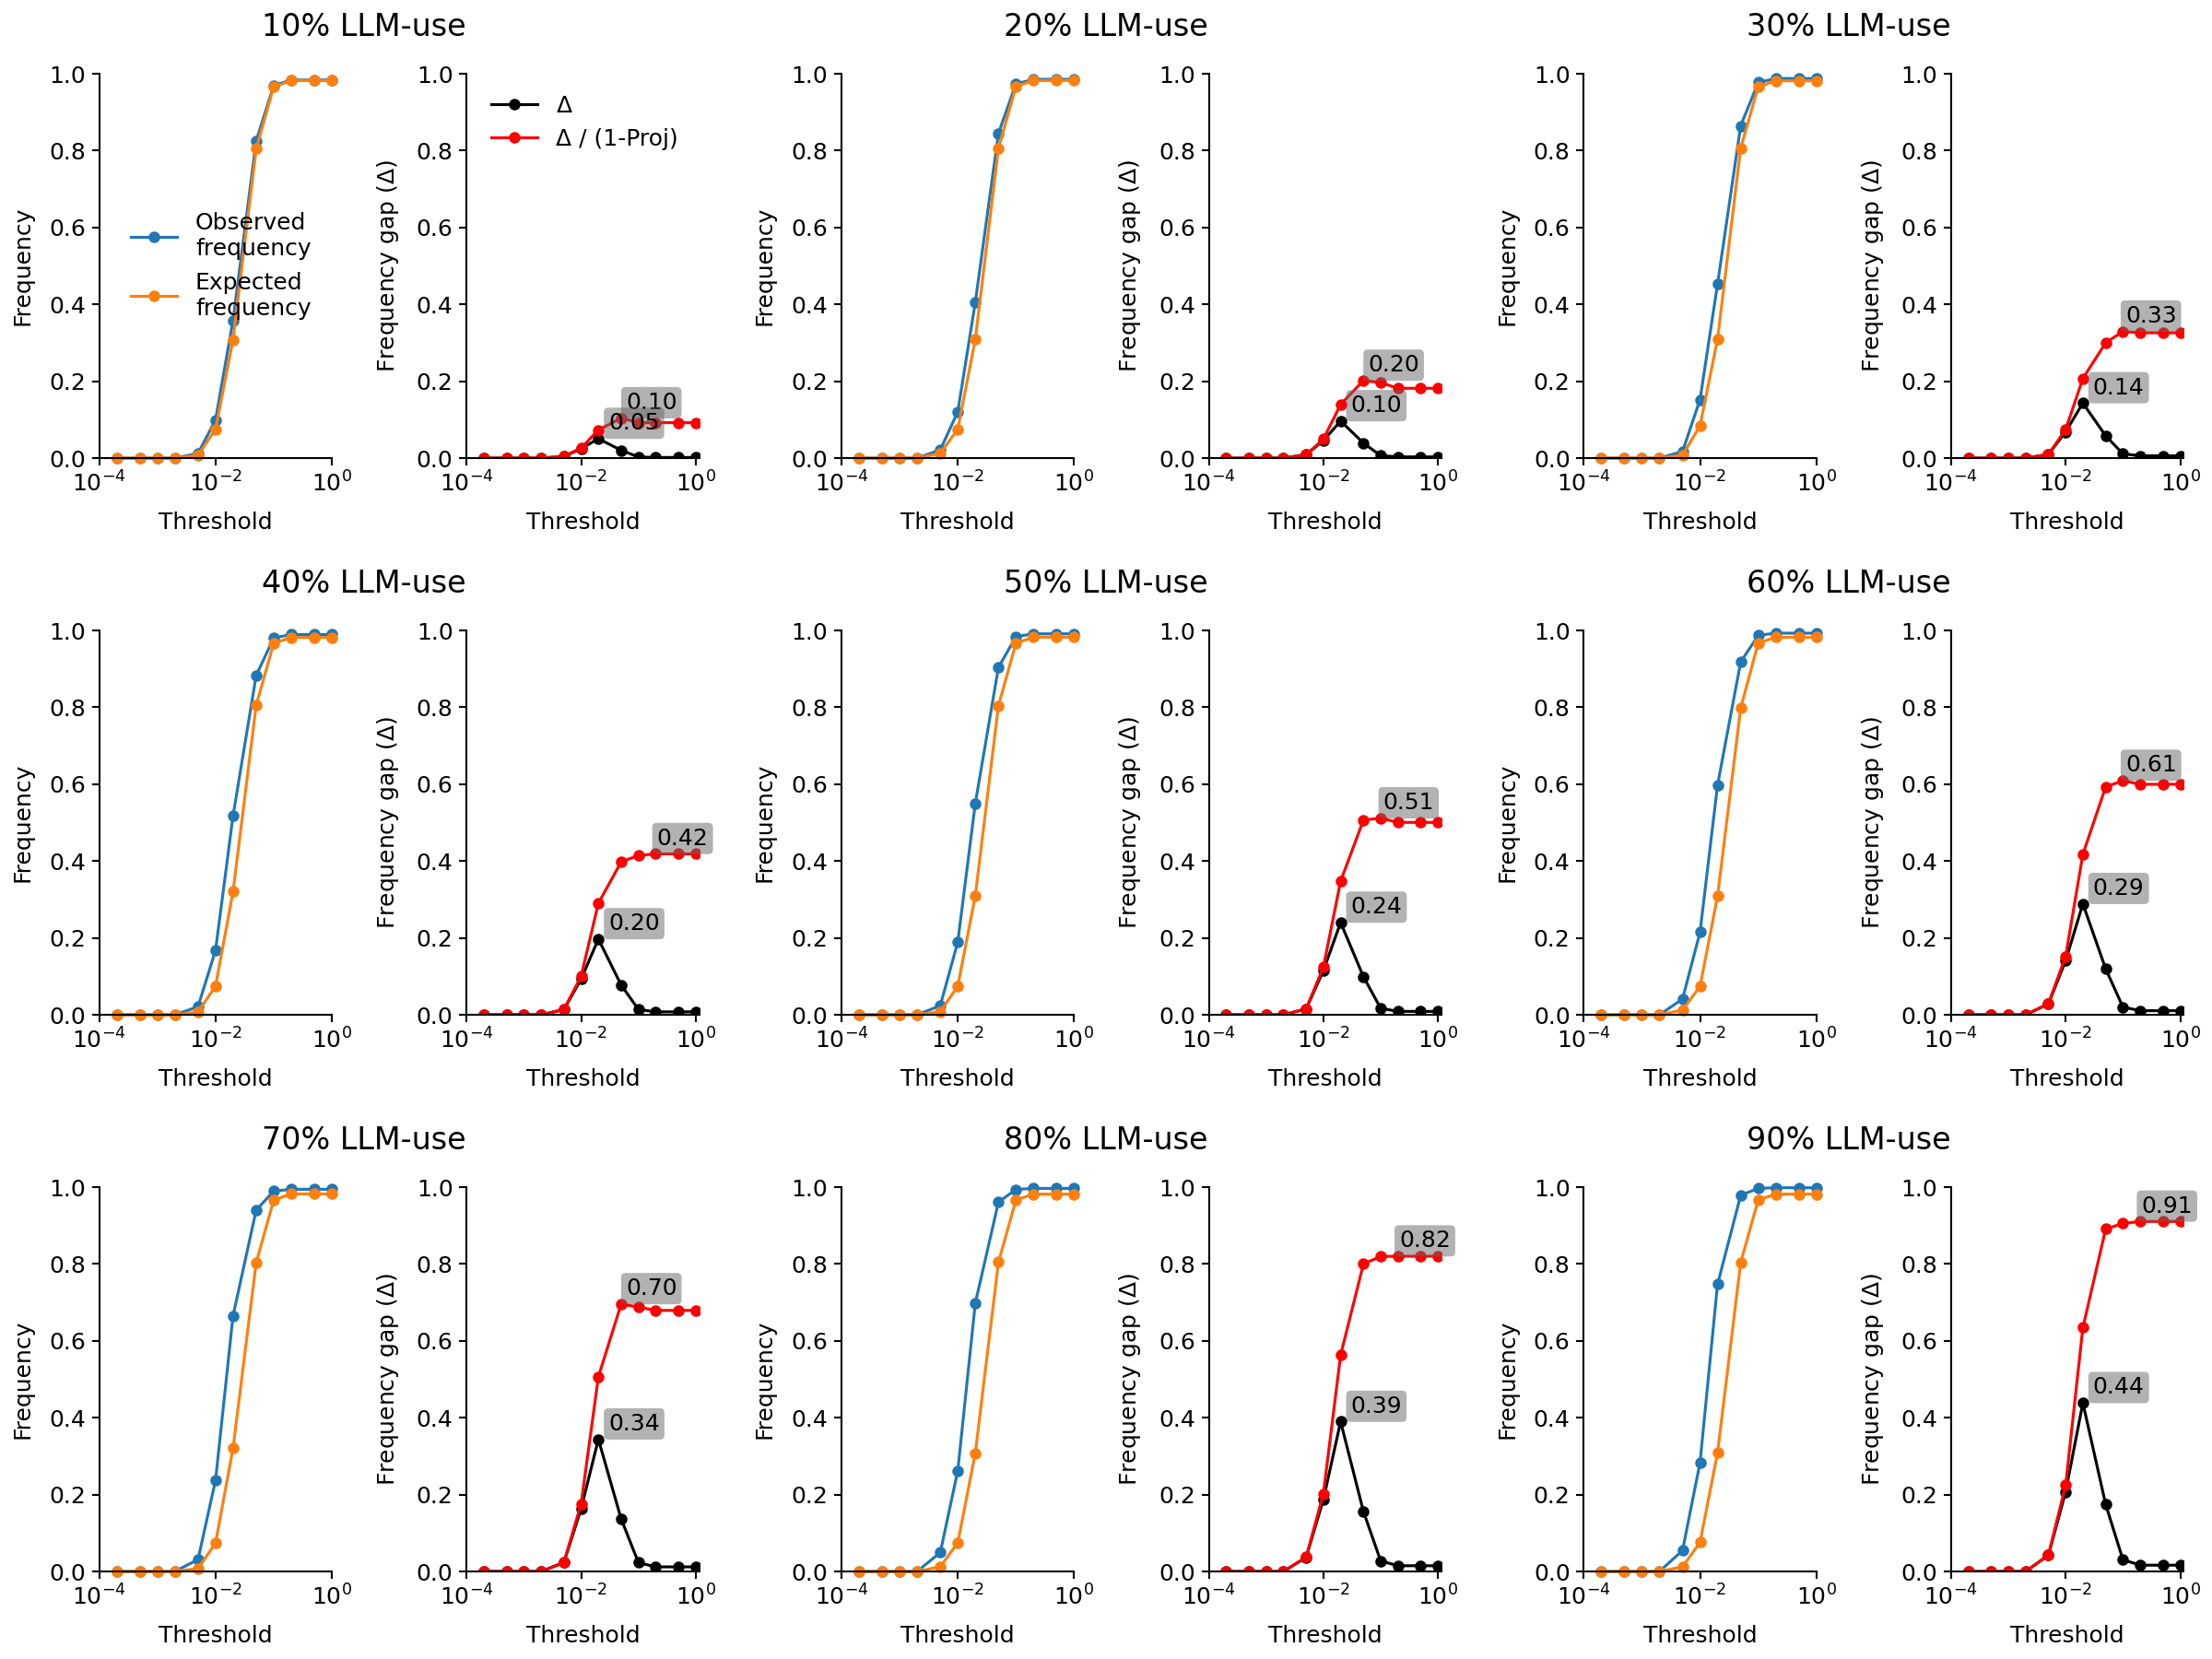
\includegraphics[width=\linewidth]{../results/plots/ground_truth_simulation/100_words.png}
    \caption{}
    \label{fig:simulation100}
\end{figure}
\begin{figure}[htbp]
    \centering
    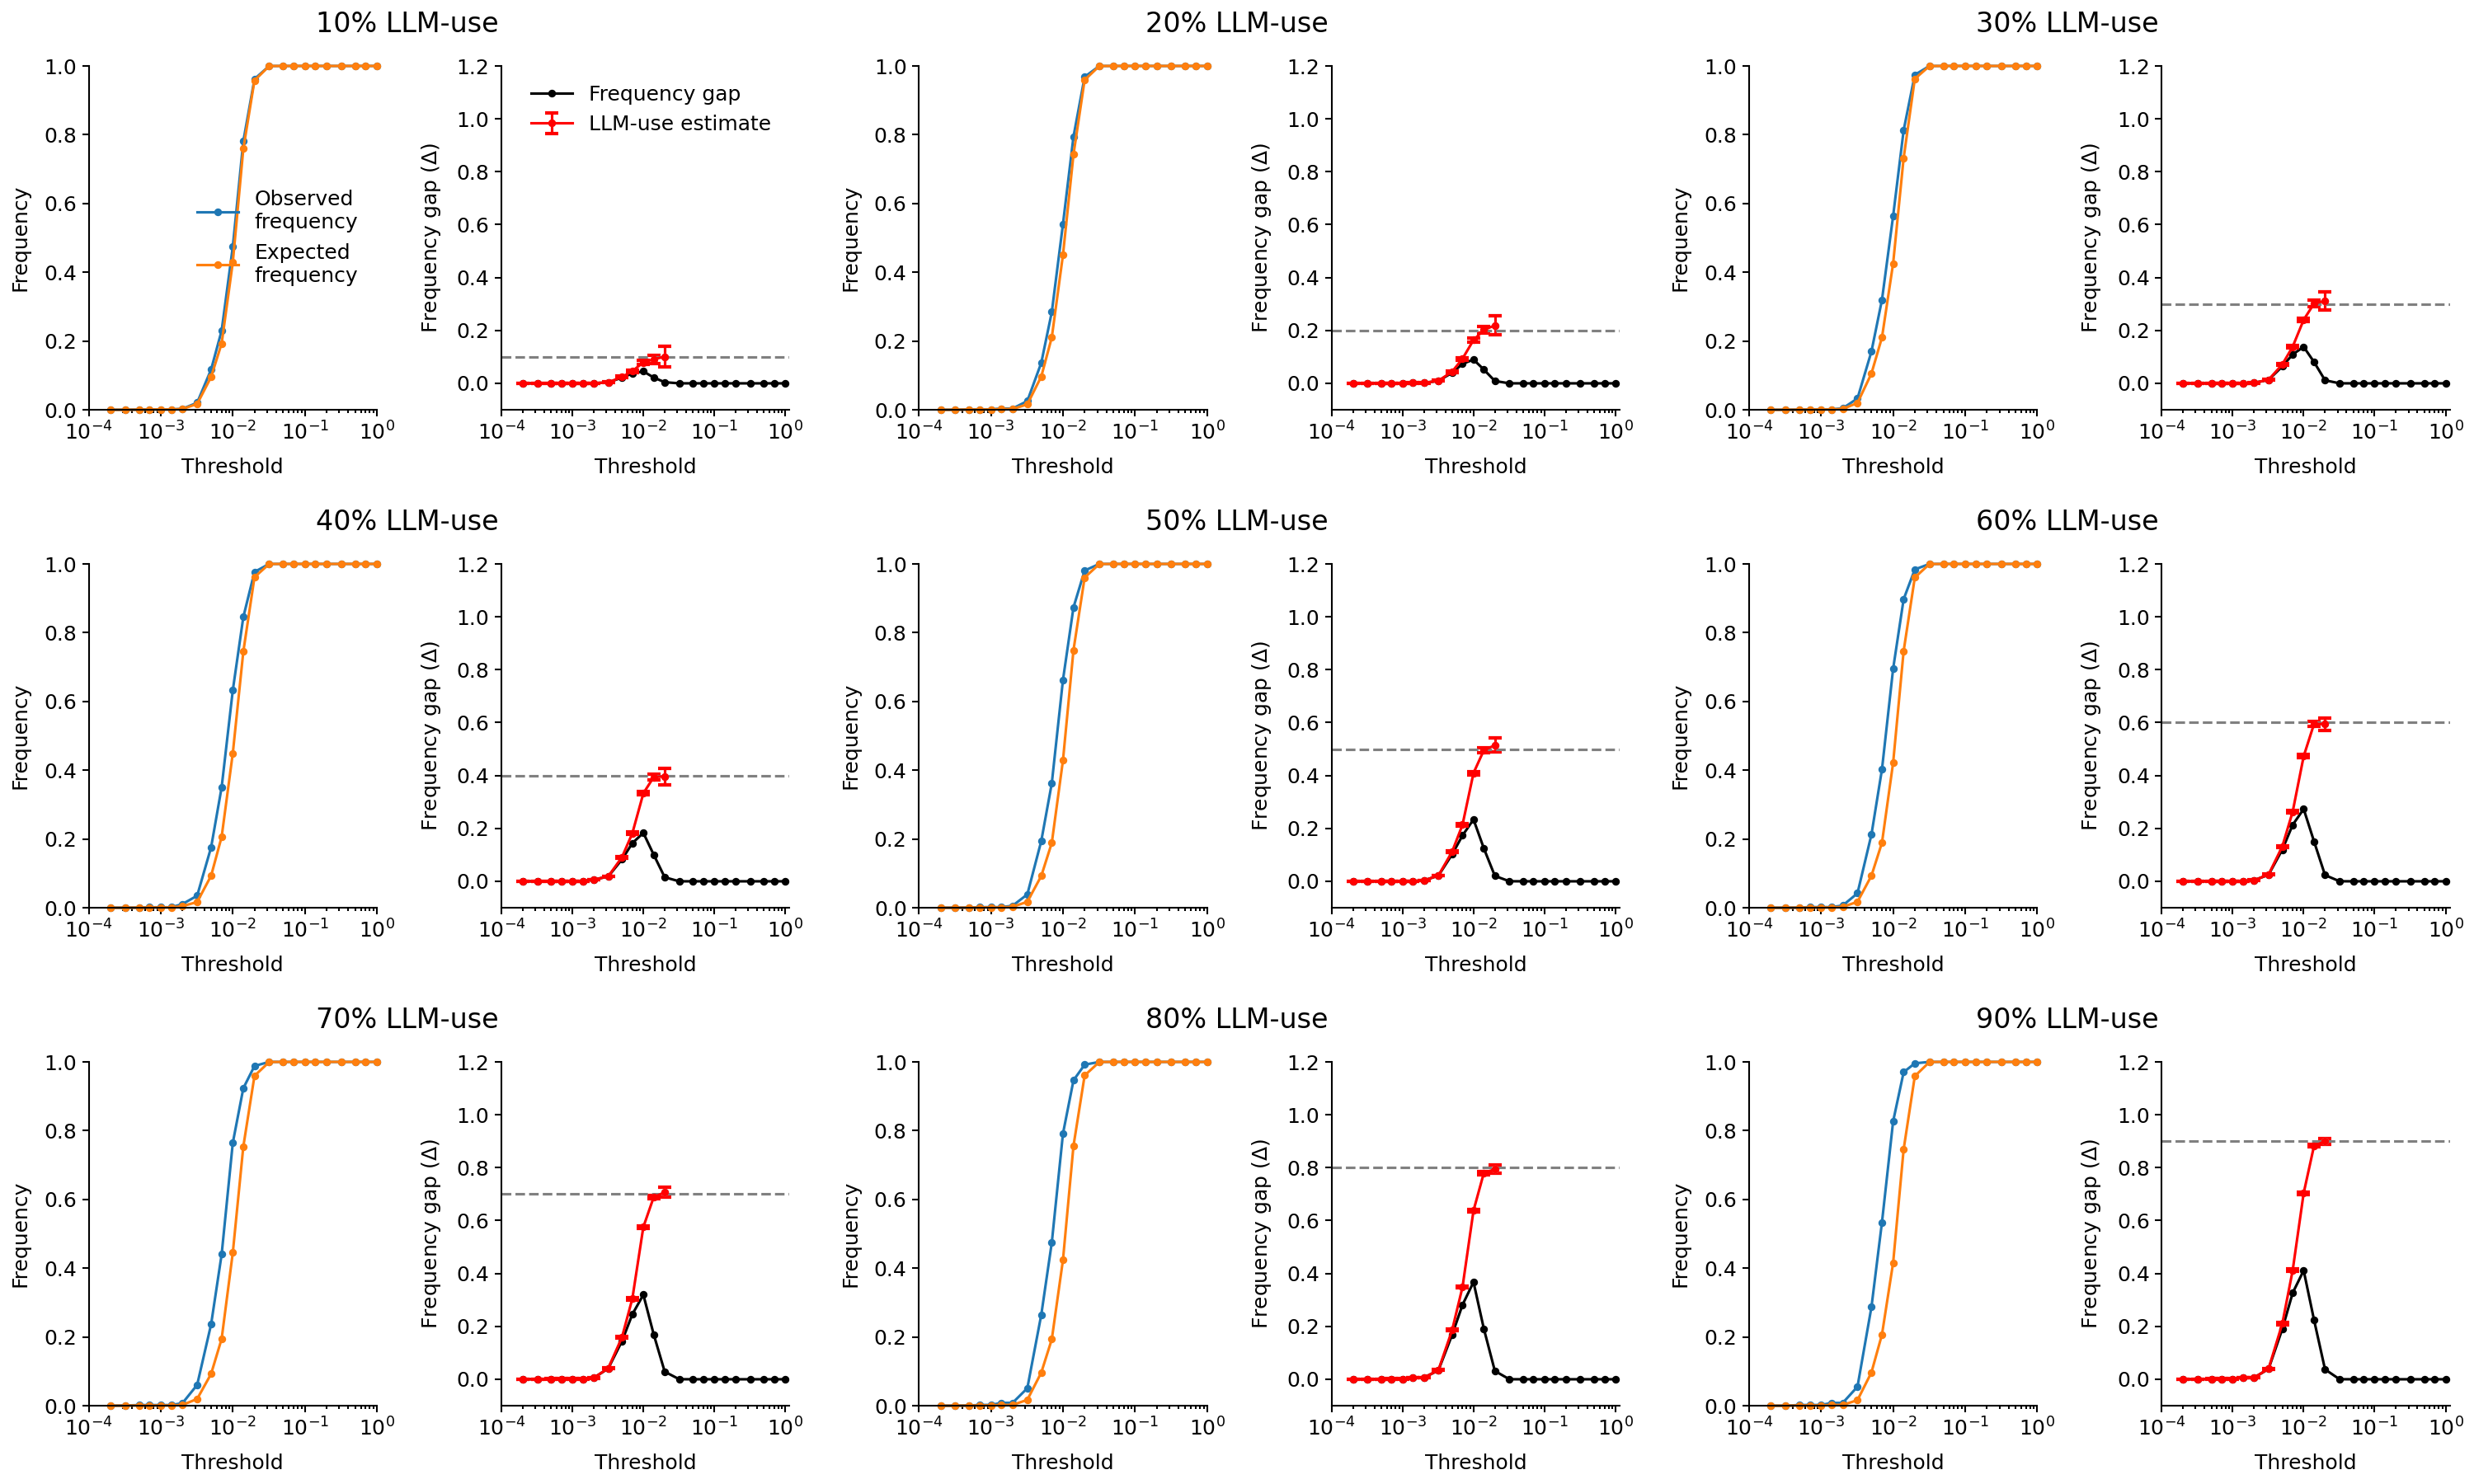
\includegraphics[width=\linewidth]{../results/plots/ground_truth_simulation/1000_words.png}
    \caption{}
    \label{fig:simulation1000}
\end{figure}
%\section{Word list optimization}\label{ap:opt}
\begin{figure}[htbp]
    \centering
    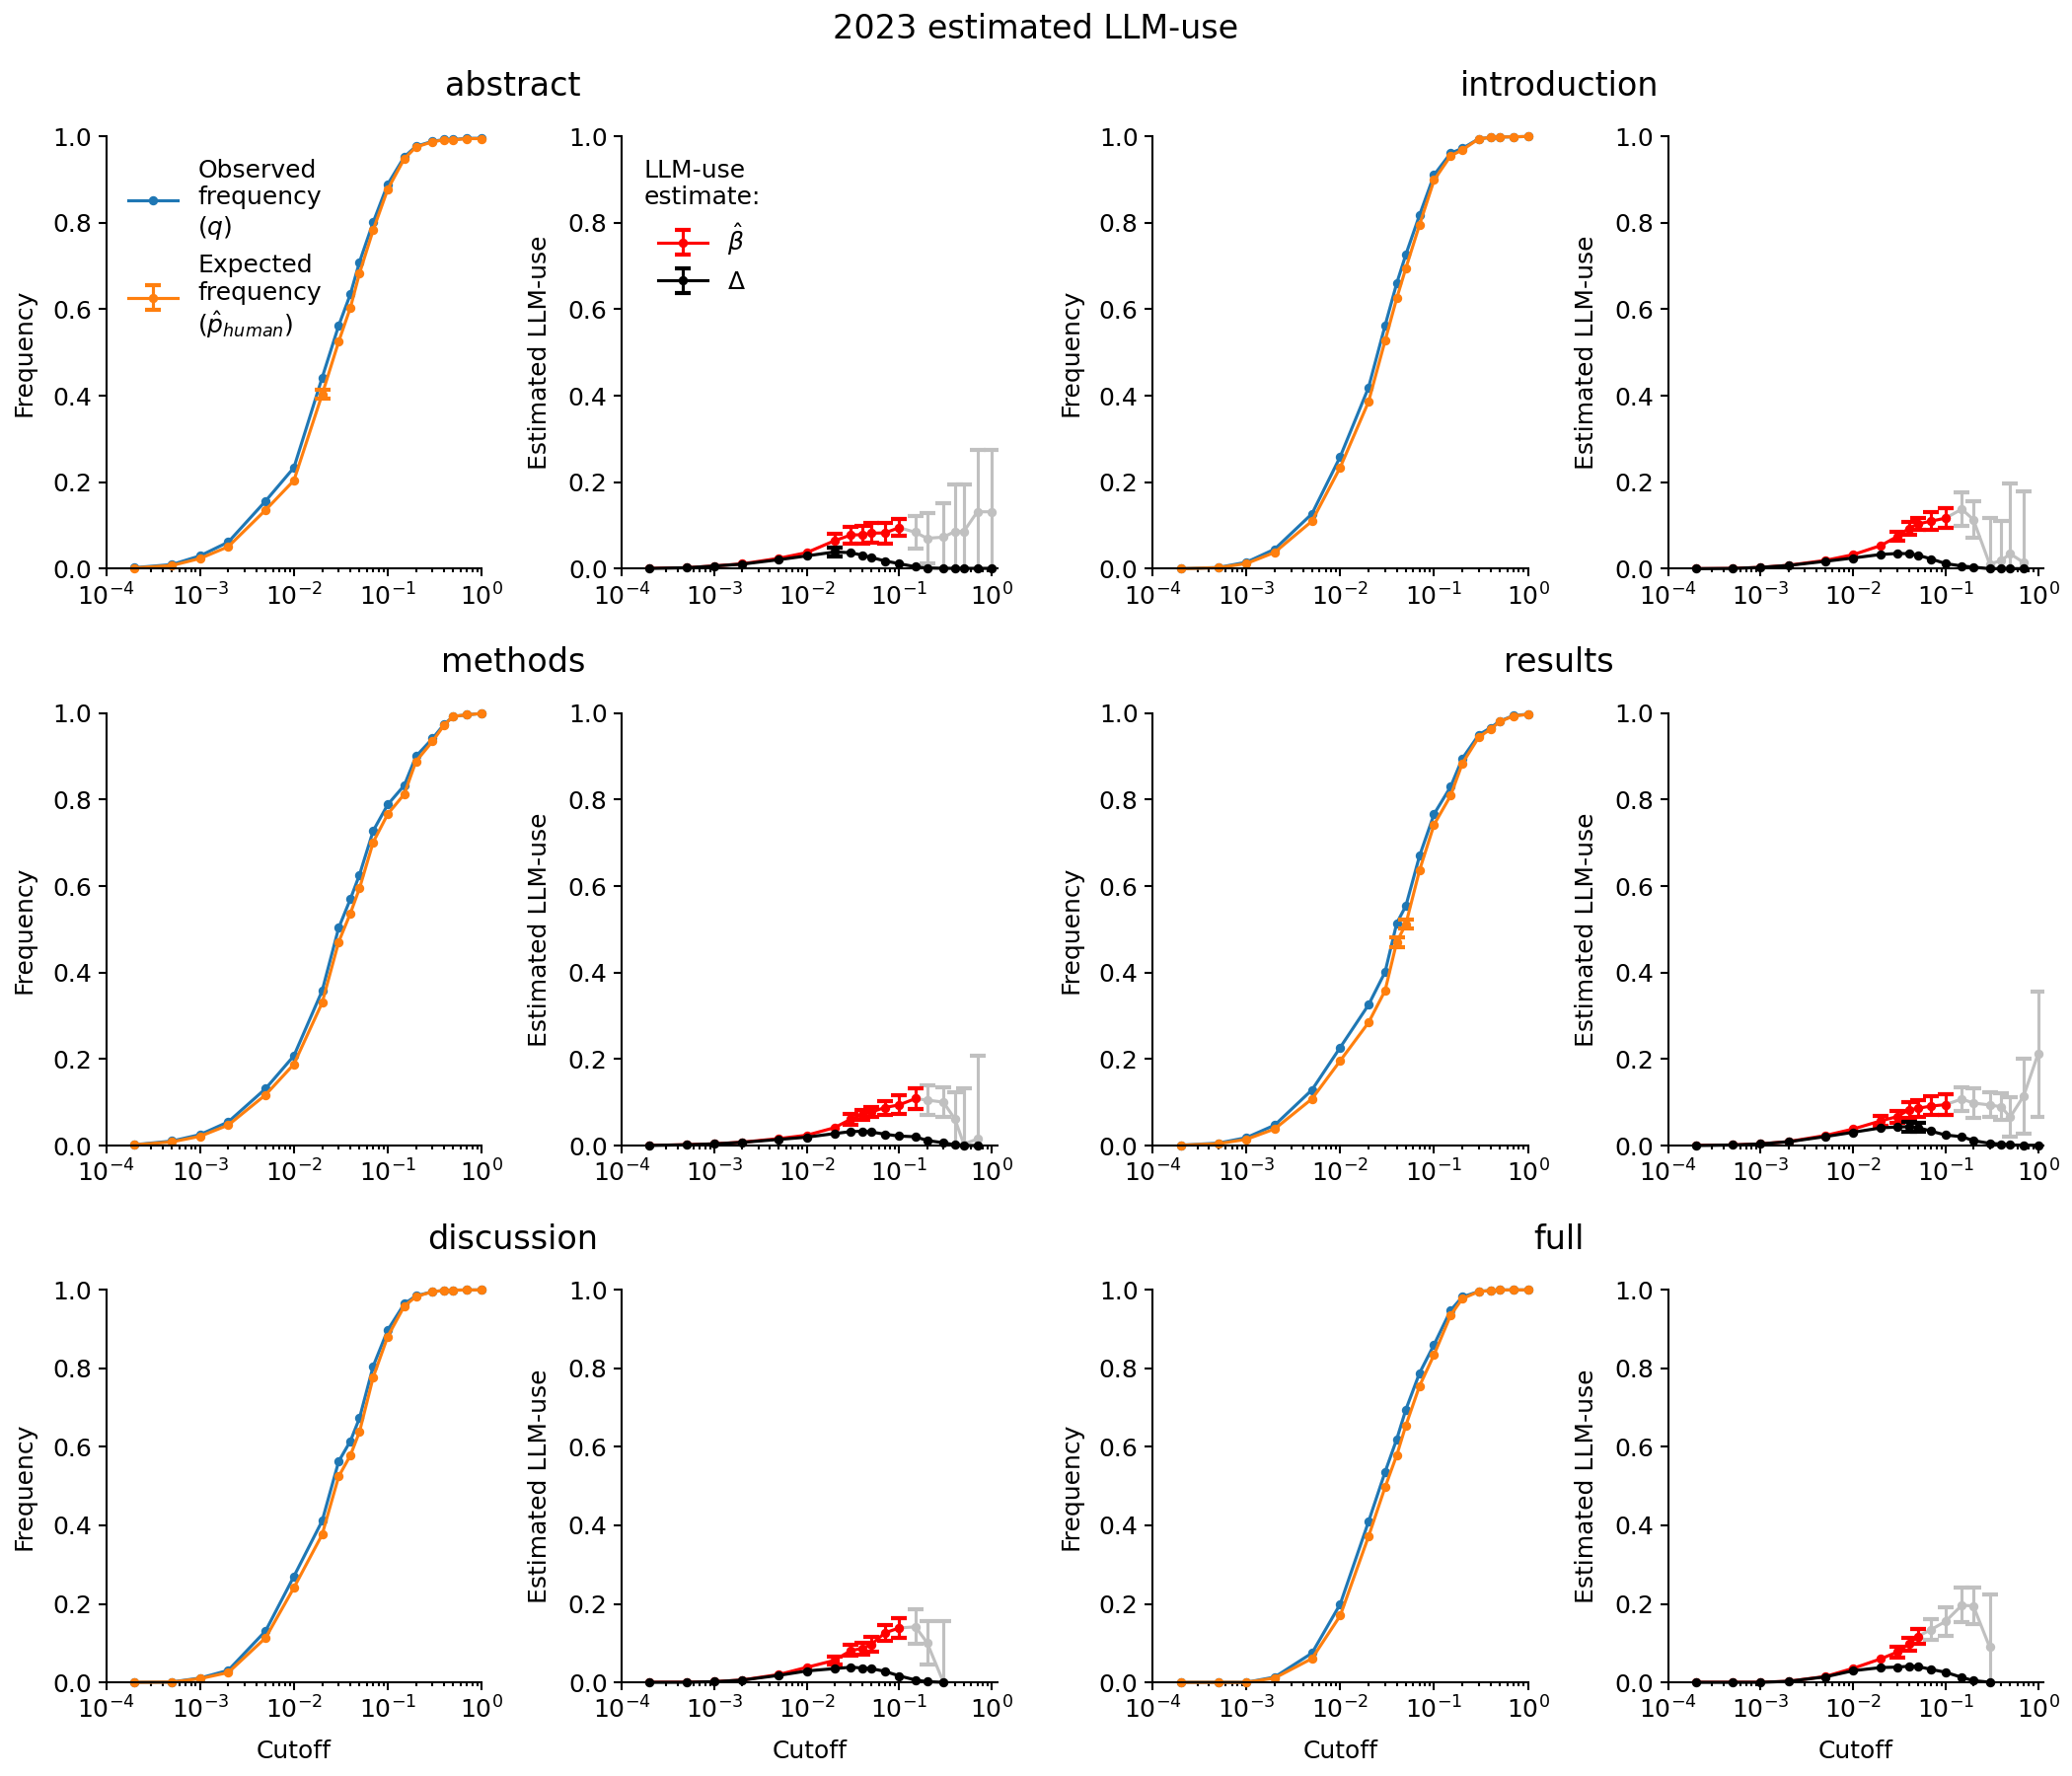
\includegraphics[width=\linewidth]{../results/plots/baseline_2026-01-23/research-article_aimrd_f/5y_2023_lower_bound_non_lemmatized_.png}
    \caption{}
    \label{fig:2023_optimization}
\end{figure}
\begin{figure}[htbp]
    \centering
    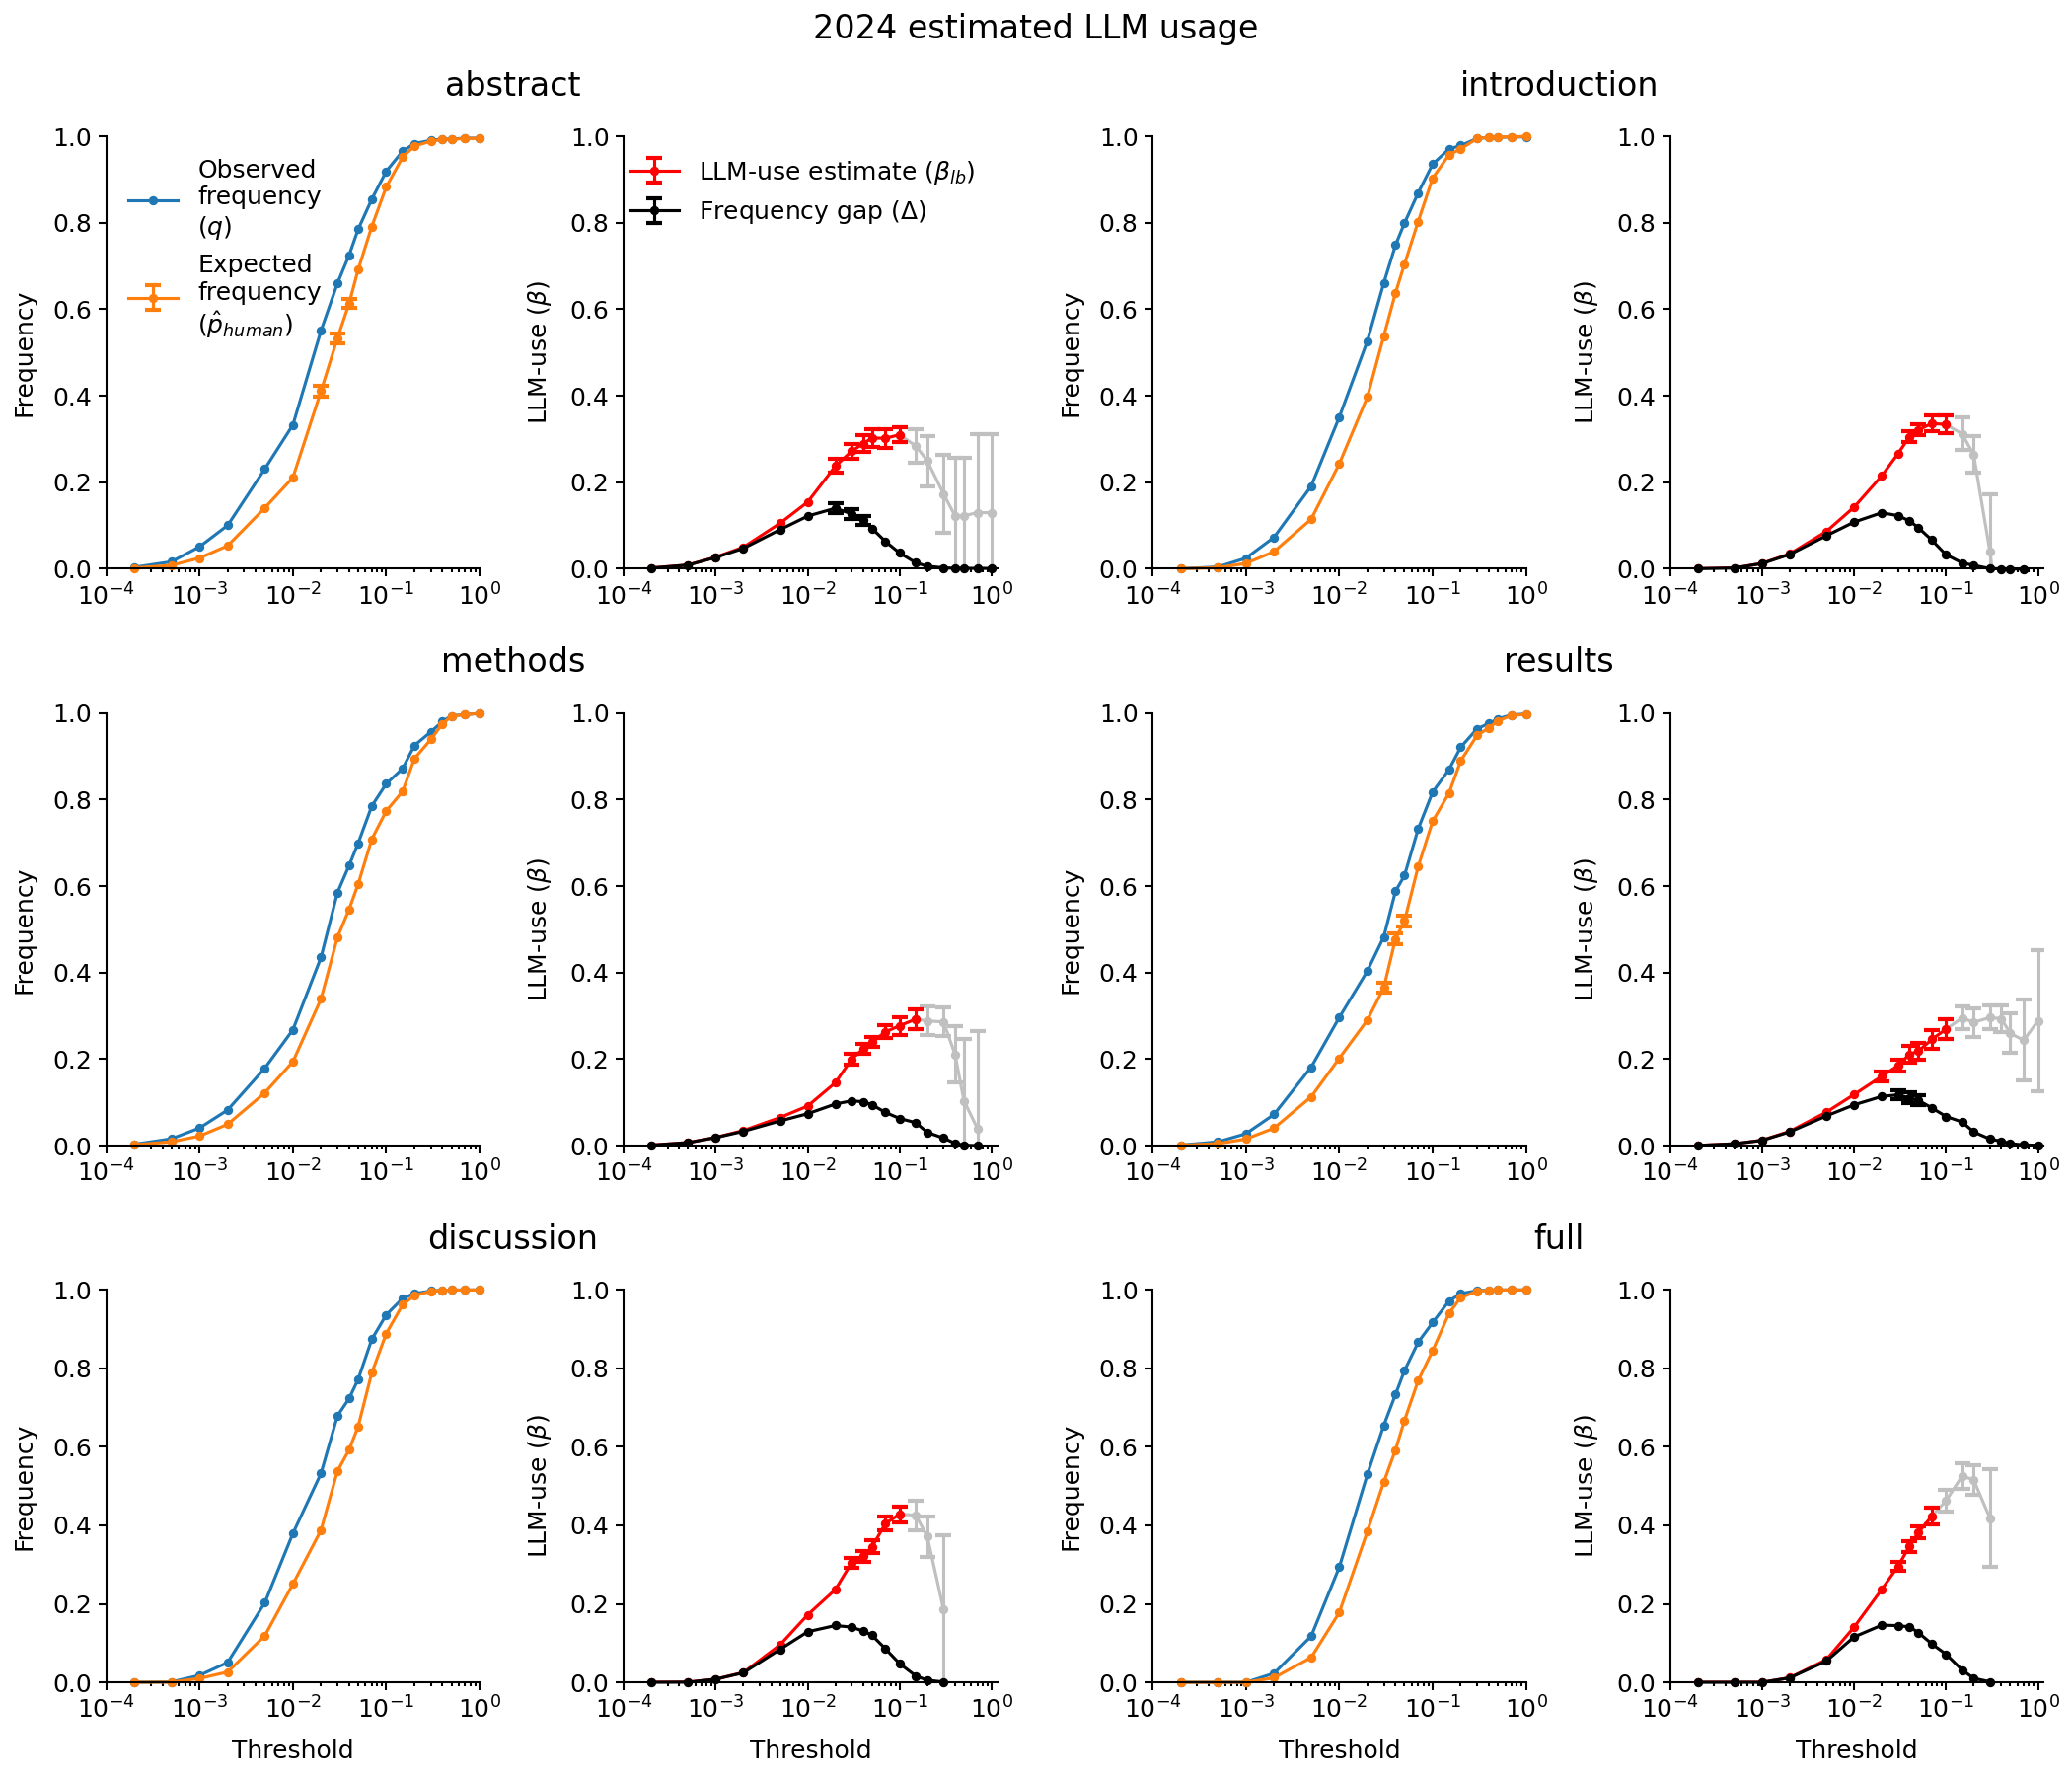
\includegraphics[width=\linewidth]{../results/plots/baseline_2026-01-23/research-article_aimrd_f/5y_2024_lower_bound_non_lemmatized_.png}
    \caption{}
    \label{fig:2024_optimization}
\end{figure}

%comment: add table with -optimal cutoff -length of resulting word list - usage estimate at optimal cutoff for all sections (+crop and sample) and all years
\begin{table}
\begin{tabular}{lrrrrrrrrr}
    \toprule
                & \mcthree{2023} & \mcthree{2024} & \mcthree{2025}\\
                & \mcone{$\hbet$} & \mcone{cutoff} & \makecell[c]{excess\\words}& \mcone{$\hbet$} & \mcone{cutoff} & \makecell[c]{excess\\words} & \mcone{$\hbet$} & \mcone{cutoff} & \makecell[c]{excess\\words} \\
    \midrule
    abstract        & 0.09 \unc{0.02} & 0.10 & 355 & 0.31 \unc{0.02} & 0.10 & 355 & 0.53 \unc{0.01} & 0.10 & 355 \\
    introduction    & 0.12 \unc{0.02} & 0.10 & 324 & 0.34 \unc{0.02} & 0.07 & 307 & 0.50 \unc{0.02} & 0.07 & 307 \\
    methods         & 0.11 \unc{0.02} & 0.15 & 348 & 0.29 \unc{0.02} & 0.15 & 348 & 0.46 \unc{0.02} & 0.15 & 348 \\
    results         & 0.09 \unc{0.02} & 0.10 & 325 & 0.27 \unc{0.02} & 0.10 & 325 & 0.47 \unc{0.02} & 0.15 & 338 \\
    discussion      & 0.14 \unc{0.02} & 0.10 & 297 & 0.43 \unc{0.02} & 0.10 & 297 & 0.68 \unc{0.01} & 0.10 & 297 \\
    full            & 0.12 \unc{0.02} & 0.05 & 211 & 0.42 \unc{0.02} & 0.07 & 232 & 0.77 \unc{0.02} & 0.20 & 296 \\
    \bottomrule
\end{tabular}
\end{table}


%\section{Subgroup analysis}
\subsection{Countries and language regions}

\begin{figure}[htbp]
    \centering
    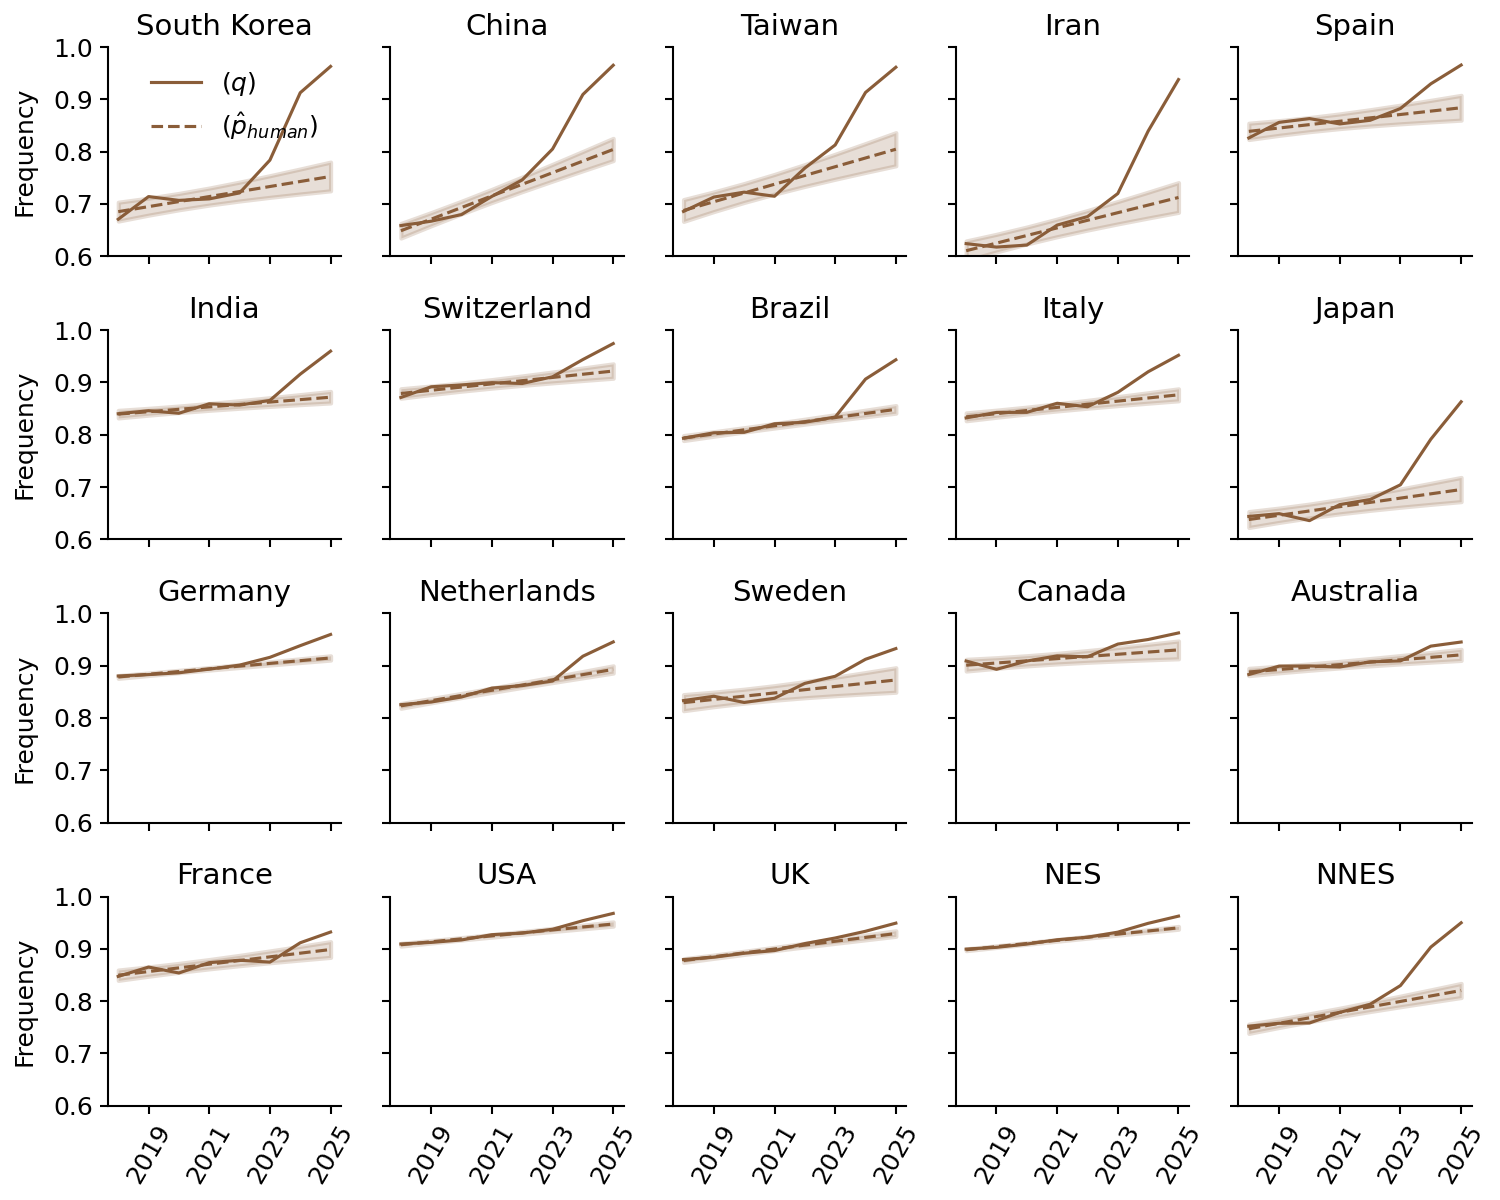
\includegraphics[width=\linewidth]{../results/plots/baseline_2026-01-23/research-article_aimrd_f/countries_individual_freqs_subsubopt.png}
    \caption{}
    \label{fig:countries_freqs}
\end{figure}

\subsection{Academic Discipline}\label{ap:disciplines}

\begin{figure}[htbp]
    \centering
    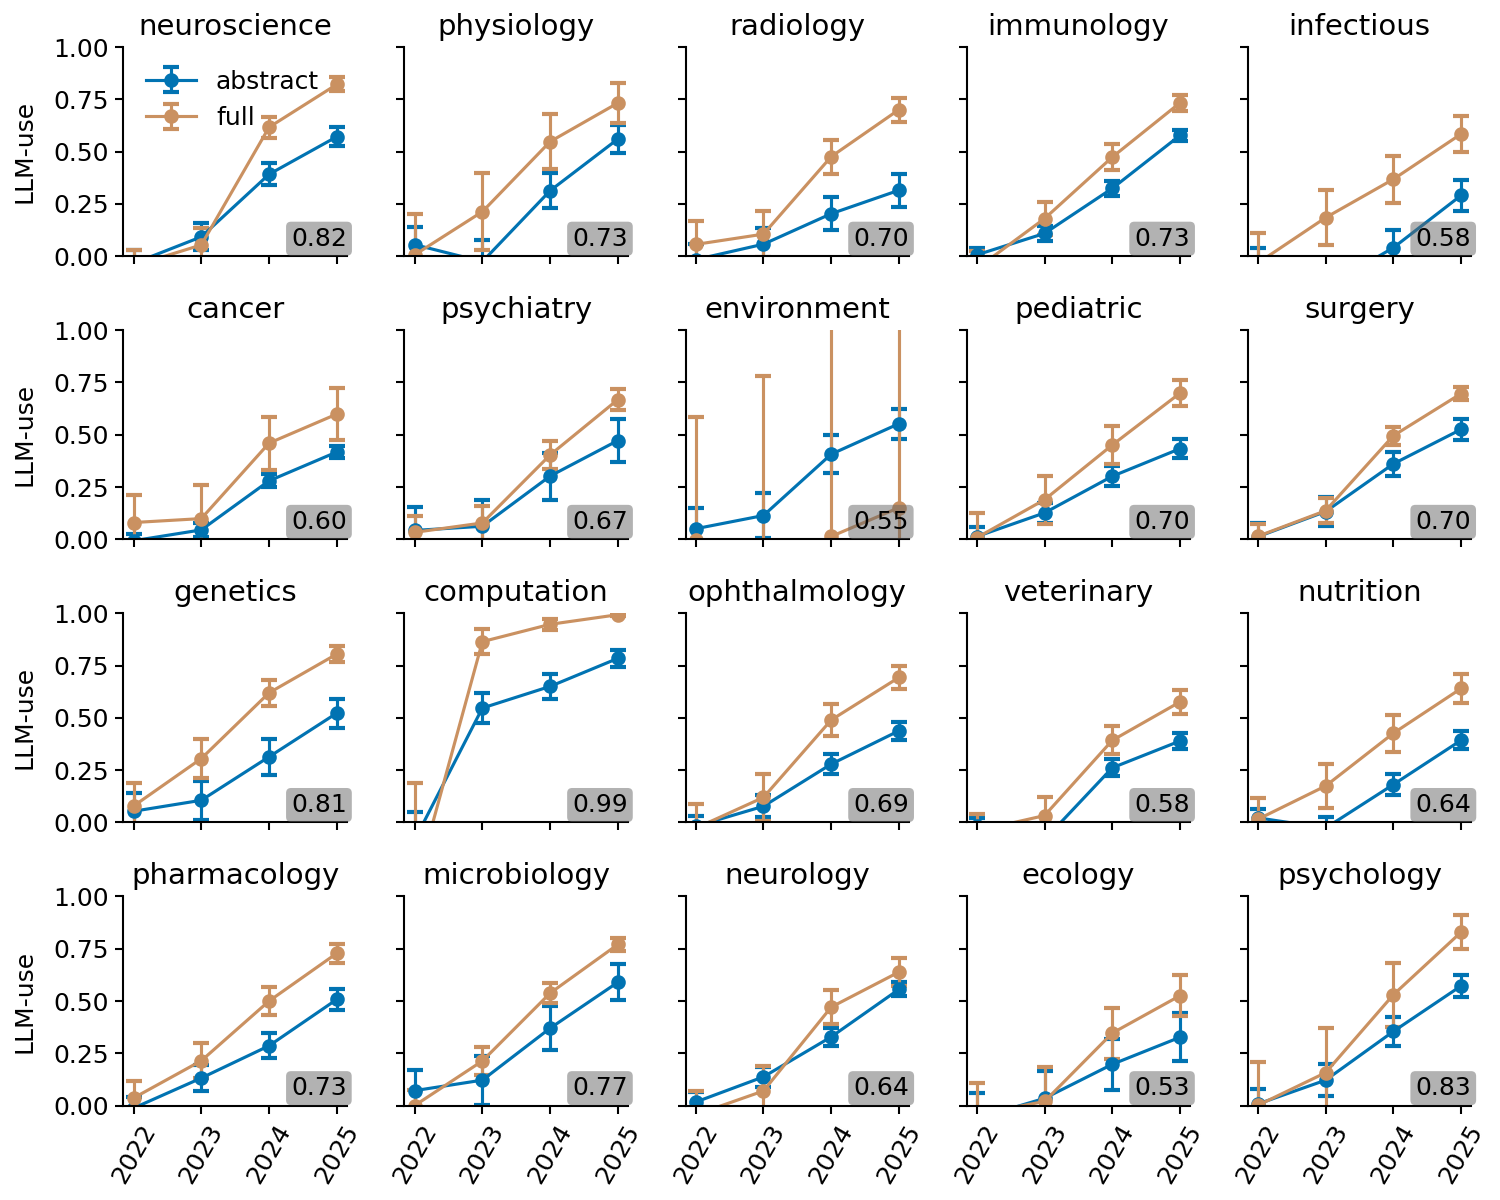
\includegraphics[width=\linewidth]{../results/plots/baseline_2026-01-23/research-article_aimrd_f/disciplines_individual.png}
    \caption{LLM-use estimates for different academic disciplines contributing to PMC for the abstract and main body of the paper. The highest estimate in each panel is marked in a gray box.}
    \label{fig:disciplines_ind}
\end{figure}

\begin{figure}[htbp]
    \centering
    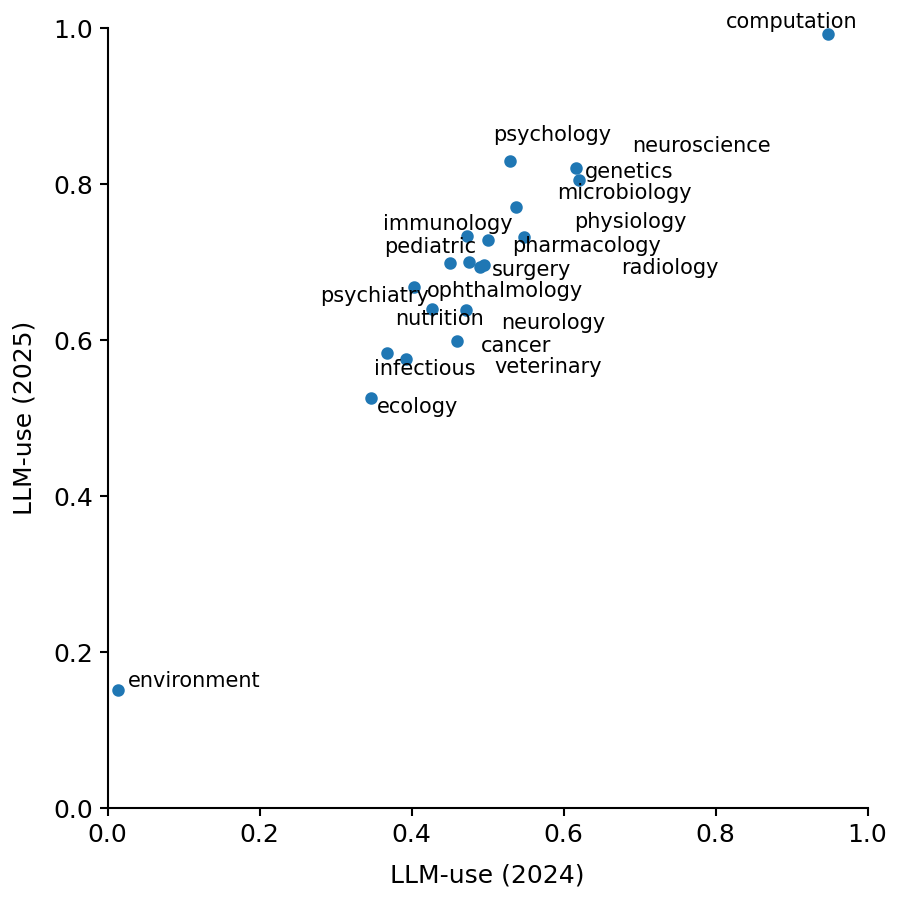
\includegraphics[width=\linewidth]{../results/plots/baseline_2026-01-23/research-article_aimrd_f/disciplines_2024v2025.png}
    \caption{LLM-use estimates of 2024 (x-axis) and 2025 (y-axis) for different academic disciplines. Because the number of papers in each category is very small, some estimates have very high uncertainty.}
    \label{fig:disciplines_all}
    %comment: this should be a different color than countries
\end{figure}

%\end{document}

